%D3 structure:
%0) D1 + D2 review (only changes)
%1) Purpose of the document
%2) Architecture Choice and language used
%   2a) Type of architecture
%   2b) Language used and why
%   2c) Database
%   2d) Dependencies
%3) User flows
%4) Code dev
%5) Team Roles

\documentclass[12pt, a4paper]{article}

% --- PACKETS ---
\usepackage{graphicx} 
\usepackage{geometry}
\usepackage{tabularx}
\usepackage{caption}
\usepackage{booktabs}
\geometry{a4paper, margin=2.5cm}
\usepackage{fancyhdr}
\usepackage[table]{xcolor}
\usepackage{hyperref}
\usepackage{xcolor} % or \usepackage{xcolor}
\usepackage{soul}
\usepackage[normalem]{ulem}
\usepackage{enumitem}
\usepackage[hypcap=false]{caption}
\newcolumntype{Y}{>{\raggedright\arraybackslash}X}
\newcolumntype{M}{>{\raggedright\arraybackslash}p{6.3cm}}

%% roba extra giorge --
\usepackage[T1]{fontenc}
\usepackage[utf8]{inputenc}
\usepackage{titlesec}
\usepackage{longtable}
\usepackage{array}
\usepackage{parskip}
\usepackage{colortbl}
\usepackage{subcaption}
\usepackage{placeins}
\usepackage{float}

\definecolor{primaryblue}{HTML}{1F3864}
\definecolor{secondaryblue}{HTML}{2E5496}
\definecolor{accentblue}{HTML}{4472C4}
\definecolor{tableheader}{HTML}{4472C4}
\definecolor{tablerowalt}{HTML}{EEF3FB}



\newcolumntype{L}[1]{>{\raggedright\arraybackslash}p{#1}}
\newcolumntype{C}[1]{>{\centering\arraybackslash}p{#1}}

%%fine roba gorge

%%roba extra giorge x2



%%

\hypersetup{
    colorlinks=true,     % Enables link coloring
    linkcolor=black,      % Color for internal links (like \nameref or \ref)
    filecolor=magenta,   % Color for local file links
    urlcolor=cyan,       % Color for web links (URLs)
    citecolor=green      % Color for bibliography citations
}



% --- SETUP HEADER E FOOTER ---
% --- DEFINIZIONE VERSIONAMENTO ---
\newcommand{\docversion}{1.0} % <-- Ho impostato la versione qui a 0.1
\pagestyle{fancy}
\fancyhf{} % Clean defaults
\fancyhead[L]{HealthMaxxin} % Top left
\fancyhead[R]{Deliverable 3 -- Architecture, User Flows, Code developement} % Top right
\fancyfoot[C]{\thepage} % Page numbering
\renewcommand{\headrulewidth}{0.4pt} % Header line
\setlength{\headheight}{15pt}

% --- TEMPLATE PER USE CASES ---
% Comando per la tabella riassuntiva (9 argomenti)
\newcommand{\usecaseheader}[9]{
    \vspace{0.5cm}
    \noindent
    \renewcommand{\arraystretch}{1.5}
    \begin{tabularx}{\textwidth}{|>{\columncolor{gray!20}\bfseries}p{4.5cm}|X|}
    \hline
    \rowcolor{blue!10}
    \multicolumn{2}{|c|}{\textbf{USE CASE #1: #2}} \\ \hline
    Goal in Context & #3 \\ \hline
    Scope \& Level & #4 \\ \hline
    Preconditions & #5 \\ \hline
    Success End Condition & #6 \\ \hline
    Failed End Condition & #7 \\ \hline
    Primary, Secondary Actors & #8 \\ \hline
    Trigger & #9 \\ \hline
    \end{tabularx}
    \par\vspace{0.2cm}
}

% Ambiente per la Description (Flusso principale)
\newenvironment{ucflow}{
    \noindent\textbf{DESCRIPTION} \par \vspace{0.1cm}
    \noindent
    \renewcommand{\arraystretch}{1.3}
    \tabularx{\textwidth}{|>{\centering\arraybackslash}p{1.2cm}|X|}
    \hline
    \rowcolor{gray!30}
    \textbf{Step} & \textbf{Action} \\ \hline
}{
    \endtabularx
    \par\vspace{0.3cm}
}

% Ambiente per le Extensions
\newenvironment{ucextensions}{
    \noindent\textbf{EXTENSIONS} \par \vspace{0.1cm}
    \noindent
    \renewcommand{\arraystretch}{1.3}
    \tabularx{\textwidth}{|>{\centering\arraybackslash}p{1.2cm}|X|}
    \hline
    \rowcolor{gray!30}
    \textbf{Step} & \textbf{Branching Action} \\ \hline
}{
    \endtabularx
    \par\vspace{0.3cm}
}

% Ambiente per le Sub-Variations
\newenvironment{ucsubvariations}{
    \noindent\textbf{SUB-VARIATIONS} \par \vspace{0.1cm}
    \noindent
    \renewcommand{\arraystretch}{1.3}
    \tabularx{\textwidth}{|>{\centering\arraybackslash}p{1.2cm}|X|}
    \hline
    \rowcolor{gray!30}
    \textbf{Step} & \textbf{Branching Action} \\ \hline
}{
    \endtabularx
    \par\vspace{0.5cm}
}

% Ambiente per i Functional Requirements (FR) collegati
\newenvironment{ucrequirements}{
    \noindent\textbf{RELATED FUNCTIONAL / NON-FUNCTIONAL REQUIREMENTS} \par \vspace{0.1cm}
    \noindent
    \renewcommand{\arraystretch}{1.3}
    \tabularx{\textwidth}{|>{\centering\arraybackslash\bfseries}p{2.5cm}|X|}
    \hline
    \rowcolor{gray!30}
    \textbf{FR/NFR ID} & \textbf{Title} \\ \hline
}{
    \endtabularx
    \par\vspace{0.5cm}
}
% Ambiente per le note di modifica / elementi editati
\newenvironment{ucedits}{
    \noindent\textbf{EDITED ITEMS} \par \vspace{0.1cm}
    \begin{quote}
}{
    \end{quote}
    \par\vspace{0.5cm}
}

\setcounter{secnumdepth}{0}

\begin{document}

% --- TITLE PAGE ---
\begin{titlepage}
    \centering
    \vspace*{2cm} 
    
    % --- PROJECT LOGO ---
    
\includegraphics[width=0.35\textwidth]{../Logo_HealthMaxxin.png} 
    
    \vspace{2.5cm} 
    
    % --- DOCUMENT TYPE ---
    {\scshape\Large Implementation\par}
    \vspace{0.2cm}
    {\large Version \docversion \par} % <-- Ora usa la variabile automatica!
    \vspace{0.5cm}
    
    % --- PROJECT TITLE ---
    {\Large\itshape HealthMaxxin\par}
    
    \vfill 
    
    % --- AUTHORS ---
    {\Large \textbf{Authors:} Federico Dapr\`{a}, Giorge Ribic, Luca Galli, Stefano Giroletti\par}
    {\Large \textbf{Group:} Cursor Maxxing\par}
    \vspace{0.5cm}
    
\end{titlepage}

% --- TABLE OF CONTENTS ---
\tableofcontents
\newpage

\phantomsection
\section{Purpose of the Document}
This document describes the implementation phase of the HealthMaxxing App, providing a detailed description of the architecture and language choices, user flows and some snippets of code. Moreover, the document also covers the improvements regarding D1 and D2, only reporting the modified sections.

\phantomsection
\section{Modifications to D1}

\phantomsection
\subsection{FR11. Identity and access management} \label{FR11}
The system shall provide identity and access management through the following functionalities:
\begin{itemize}
    \item \textbf{FR11.1 \hl{Patient} registration:} The system shall allow unregistered patients to create a new account using their email by providing the personal data required for identification, verification and service usage.

    \item \textbf{FR11.2 \hl{Patient} validation:} The system shall allow newly registered patients to validate their accounts by verifying a secure token sent to their registered email address.

    \item \textbf{FR11.3 User login:} The system shall allow registered users in the standard User hierarchy to authenticate and securely access their accounts using their registered email and password credentials, or alternatively through national digital identity providers (e.g., SPID, CIE).

    \item \textbf{FR11.4 \hl{System Administrator authentication}:} The system shall allow an active account with administrative privileges to authenticate through the dedicated administration interface using its email address and password. 
\end{itemize}
\vspace{0.3cm}

The term "User" has been replaced with "Patient" in FR11.1 and FR11.2 because registration and validation apply specifically to patients. FR11.3 remains applicable to the standard User hierarchy defined in D2. FR11.4 is a new functional requirement introduced during implementation to document the separate System Administrator authentication flow, which was implemented but not covered by FR11.3.



\phantomsection
\section{Modifications to D2}

\phantomsection
\addcontentsline{toc}{subsection}{UC2. Create Insurance Policy}
\hypertarget{UC2}{}
\usecaseheader
  {UC2}  % 1: ID
  {Create Insurance Policy} % 2: Titolo
  {To enable the System Administrator to create new insurance policies shared across all facilities in the healthcare
network.} % 3: Goal
  {Scope: Global Insurance Policy handling. Level: Primary.} % 4: Scope
  {The user is logged in as a System Admin.} % 5: Preconditions
  {A new Insurance Policy is created.} % 6: Success
  {The System remains unchanged. The System returns an error.} % 7: Failed
  {Primary: System Admin. Secondary: Database.} % 8: Actors
  {The System Admin asks the System to create a new Insurance Policy.} % 9: Trigger
\begin{ucrequirements}
    FR9.1 & Create insurance policy \\ \hline
    NFR4 & Scalability and capacity \\ \hline     
\end{ucrequirements}
\begin{ucflow}
    1 & The System Admin asks the System to create a new Insurance Policy. \\ \hline
    2 & The System Admin fills in the required fields. \\ \hline
    3 & The System Admin saves. \\ \hline
    4 & The System checks if the discount percentage is a valid amount. \\ \hline
    5 & \hl{The System checks if the maximum coverage is a valid amount.} \\\hline
    6 & The System creates the new Insurance Policy in the Database. \\ \hline
    7 & The System returns a success message. \\ \hline
\end{ucflow}

\begin{ucextensions}
    3a & \textbf{The System Admin cancels:}\newline 
         1. The System aborts the creation process.\newline 
         2. Use case ends. \\ \hline
    4a & \textbf{Validity check fails:}\newline 
         1. The System identifies an invalid amount for the discount percentage.\newline 
         2. The System returns an error.\newline 
         3. Go to main flow step 2 to perform a correction. \\ \hline
    \rowcolor{yellow}
    5a & \textbf{Validity check fails:}\newline 
         1. The System identifies an invalid amount for the maximum coverage.\newline 
         2. The System returns an error.\newline 
         3. Go to main flow step 2 to perform a correction. \\ \hline
\end{ucextensions}
\begin{ucedits}
Added a backend validity check for the maximum coverage amount (steps 5 and 5a). 
The check was already implemented in the system but had not been explicitly documented in this use case.
\end{ucedits}


\phantomsection
\addcontentsline{toc}{subsection}{UC6. Update Insurance Policy}
\hypertarget{UC6}{}
\usecaseheader
  {UC6}  % 1: ID
  {Update Insurance Policy} % 2: Titolo
  {To enable the System Administrator to edit an existing insurance policies shared across all facilities in the healthcare
network.} % 3: Goal
  {Scope: Global Insurance Policy handling. Level: Primary.} % 4: Scope
  {The user is logged in as a System Admin.} % 5: Preconditions
  {An existing Insurance Policy is edited.} % 6: Success
  {The System remains unchanged. The System returns an error.} % 7: Failed
  {Primary: System Admin. Secondary: Database.} % 8: Actors
  {The System Admin asks the System to edit an existing Insurance Policy.} % 9: Trigger
\begin{ucrequirements}
        FR9.3 & Update insurance policy \\ \hline 
\end{ucrequirements}
\begin{ucflow}
    1 & The System Admin asks the System to update an existing Insurance Policy. \\ \hline
    2 & The System Admin fills in the required fields. \\ \hline
    3 & The System Admin saves. \\ \hline
    4 & The System checks if the discount percentage is a valid amount. \\ \hline
    5 & \hl{The System checks if the maximum coverage is a valid amount.} \\\hline
    6 & The System updates the Insurance Policy in the Database. \\ \hline
    7 & The System returns a success message. \\ \hline
\end{ucflow}

\begin{ucextensions}
    3a & \textbf{The System Admin cancels:}\newline 
         1. The System aborts the editing process.\newline 
         2. Use case ends. \\ \hline
    4a & \textbf{Validity check fails:}\newline 
         1. The System identifies an invalid amount for the discount percentage.\newline 
         2. The System returns an error.\newline 
         3. Go to main flow step 2 to perform a correction. \\ \hline
    
    \rowcolor{yellow}
    5a & \textbf{Validity check fails:}\newline 
         1. The System identifies an invalid amount for the maximum coverage.\newline 
         2. The System returns an error.\newline 
         3. Go to main flow step 2 to perform a correction. \\ \hline
\end{ucextensions}
\begin{ucedits}
Added a backend validity check for the maximum coverage amount (steps 5 and 5a). The check was already implemented during Insurance Policy updates but had not been explicitly documented in this use case.
\end{ucedits}

\phantomsection
\addcontentsline{toc}{subsection}{UC10. Cancel appointment (Patient)}
\hypertarget{UC10}{}
\usecaseheader
  {UC10}  % 1: ID
  {Cancel appointment (Patient)} % 2: Titolo
  {To enable Patient to cancel a booked medical appointment} % 3: Goal
  {Scope: Appointment management. Level: Primary.} % 4: Scope
  {The Patient is logged in.} % 5: Preconditions
  {An existing medical appointment is deleted.} % 6: Success
  {The System remains unchanged. The System returns an error.} % 7: Failed
  {Primary: Patient. Secondary: Database, Payment Service, Mail Service.} % 8: Actors
  {Patient asks the System to cancel a booked appointment.} % 9: Trigger
\begin{ucrequirements}
    FR16.2 & Cancel appointment (Patient) \\ \hline
    \end{ucrequirements}
\begin{ucflow}
    1 & Patient asks the System to cancel a booked appointment. \\ \hline
    2 & The System asks for confirmation. \\ \hline
    3 & The Patient confirms. \\ \hline
    4 & The System performs validity check. \\ \hline
    5 & The System cancels the appointment. \\ \hline
    6 & The Patient is refunded. \\\hline
    7 & \hl{The System sends a cancellation email.} \\\hline
\end{ucflow}

\begin{ucextensions}
    3a & \textbf{The Patient cancels:}\newline 
         1. The System aborts the editing process.\newline 
         2. Use case ends. \\ \hline
    4a & \textbf{Late canceling:}\newline 
         1. The System identifies that the appointment is in less than 48 hours.\newline 
         2. Cancellation is aborted.\newline 
         3. The System returns an error.\newline 
         4. Use case ends. \\ \hline
    6a & \textbf{Appointment not paid:}\newline 
         1. The System checks if the appointment was paid ahead.\newline 
         2. If not, proceed to step 7 (refund is skipped).\\ \hline
\end{ucextensions}
\begin{ucedits}
Added the appointment cancellation email notification (step 7) to align the use case with the actual system behavior and ensure that patient communications are explicitly documented.
\end{ucedits}

\phantomsection
\addcontentsline{toc}{subsection}{UC12. Register Doctor}
\hypertarget{UC12}{}
\usecaseheader
  {UC12} % 1: ID
  {Register Doctor} % 2: Titolo
  {A System Admin wants to add a new Doctor to the hospital’s digital infrastructure.} % 3: Goal
  {Scope: Hospital structures handling. Level: Primary.} % 4: Scope
  {The user is logged in as a System Admin. \sout{The relevant hospital structure already exists.}} % 5: Preconditions
  {The Doctor is successfully saved in the Database, and a set of one-time credentials is provided to the System Admin.} % 6: Success
  {The registration is aborted due to invalid data or duplication; no credentials are created.} % 7: Failed
  {Primary: System Admin. Secondary: Database.} % 8: Actors
  {The System Admin asks the System to create a new Doctor account.} % 9: Trigger

\begin{ucrequirements}
    FR1.7 & Doctor registration \\ \hline
    NFR4 & Scalability and capacity \\ \hline
\end{ucrequirements}

\begin{ucflow}
    1 & The System Admin asks the System to create a new Doctor account. \\ \hline
    2 & The System Admin fills in the required fields, including Doctor's personal data. \\ \hline
    3 & The System Admin saves. \\ \hline
    4 & The System checks if the \hl{fiscal code} field is not duplicate. \\ \hline
    5 & The System creates the new Doctor account in the Database. \\ \hline
    6 & The System returns the new account credentials, which are displayed just once. \\ \hline
\end{ucflow}

\begin{ucextensions}
    3a & \textbf{The System Admin cancels:}\newline 
         1. The System aborts the creation process.\newline 
         2. Use case ends. \\ \hline
    4a & \textbf{Validity check fails:}\newline 
         1. The System identifies duplicated personal data for the Doctor.\newline 
         2. The System returns an error.\newline 
         3. Go to main flow step 2 to perform a correction. \\ \hline
\end{ucextensions}

\begin{ucedits}
Removed the precondition requiring the relevant hospital structure to already exist, as it is not necessary for Doctor registration. 
Replaced the uniqueness check from "name" to "fiscal code" to correctly identify duplicate Doctor records using a unique identifier.
\end{ucedits}

\phantomsection
\addcontentsline{toc}{subsection}{UC13. Assign Doctor to Hospital}
\hypertarget{UC13}{}
\usecaseheader
  {UC13} % 1: ID
  {Assign Doctor to Hospital} % 2: Titolo
  {To enable the System Administrator to assign a registered Doctors to a specific hospital.} % 3: Goal
  {Scope: Hospital structures handling. Level: Primary.} % 4: Scope
  {The user is logged in as a System Admin. The target hospital exists. The Doctors are registered in the System.} % 5: Preconditions
  {The selected Doctors are successfully assigned to the selected hospital.} % 6: Success
  {The assignment fails; previous assignments remain unchanged.} % 7: Failed
  {Primary: System Admin, Head of Hospital. Secondary: Database.} % 8: Actors
  {The user selects Doctors and assigns them to a hospital.} % 9: Trigger


\begin{ucrequirements}
    FR1.8 & Doctor assignment \\ \hline
    NFR4 & Scalability and capacity \\ \hline
\end{ucrequirements}


\begin{ucflow}
    1 & The System Admin selects one or more Doctors from the set of registered Doctors. \\ \hline
    2 & The System Admin selects the target hospital. \\ \hline
    3 & The System Admin requests assignment. \\ \hline
    4 & The System checks whether selected Doctors are already assigned to a hospital. \\ \hline
    5 & The System displays current assignment status (including any existing hospital assignments). \\ \hline
    6 & The System Admin confirms or modifies the selection. \\ \hline
    7 & The System assigns the Doctors to the selected hospital and updates the System status. \\ \hline
\end{ucflow}


\begin{ucextensions}
    3a & \textbf{Cancel operation:}\newline 
         1. The System Admin cancels the assignment.\newline 
         2. No changes are made to the System.\newline 
         3. Use case ends. \\ \hline

    6a & \textbf{System Admin does not confirm assignment:}\newline 
         1. The System Admin rejects the proposed assignment or modifies the selection.\newline 
         2. The System returns to step 1 or 2 depending on modification.\newline 
         3. Use case continues or ends. \\ \hline
\end{ucextensions}


\begin{ucedits}
Moved validity checking of existing assignments before confirmation, so the System Admin is informed of current Doctor allocation status prior to final confirmation.
\end{ucedits}   


\phantomsection
\addcontentsline{toc}{subsection}{UC14. Appoint Head of Hospital}
\hypertarget{UC14}{}
\usecaseheader
  {UC14} % 1: ID
  {Appoint Head of Hospital} % 2: Titolo
  {To enable the System Administrator to appoint a Registered Doctor to the strategic role of Head of Hospital for a specific facility.} % 3: Goal
  {Scope: Hospital structures handling. Level: Primary.} % 4: Scope
  {The user is logged in as a System Administrator. The specific hospital has been created. The Doctor is already registered in the System.} % 5: Preconditions
  {The selected Doctor is successfully appointed as Head of Hospital.} % 6: Success
  {The appointment fails; the System state remains unchanged and the previous head (if any) remains in place.} % 7: Failed
  {Primary: System Administrator. Secondary: Database.} % 8: Actors
  {The System Administrator wants to appoint a Doctor as Head of Hospital.} % 9: Trigger


\begin{ucrequirements}
    FR2 & Strategic role appointment (Head of Hospital) \\ \hline
\end{ucrequirements}


\begin{ucflow}
    1 & The System Administrator selects a Doctor from the list of Registered Doctors. \\ \hline
    2 & The Admin saves the selection. \\ \hline
    3 & The System prompts a confirmation message including the currently assigned Head of Hospital (if any). \\ \hline
    4 & The Admin confirms the replacement. \\ \hline
    5 & The System performs validity checks. \\ \hline
    6 & The Doctor is appointed as Head of Hospital and the System status is updated. \\ \hline
\end{ucflow}


\begin{ucextensions}
    2a & \textbf{Operation canceled:}\newline 
         1. Admin cancels the operation.\newline 
         2. No changes are made to the Database.\newline 
         3. Use case ends. \\ \hline

    5a & \textbf{Doctor not found:}\newline 
         1. System cannot find the selected Doctor.\newline 
         2. Operation is aborted.\newline 
         3. System returns an error.\newline 
         4. Use case ends. \\ \hline
\end{ucextensions}


\begin{ucedits}
Removed extension 2a ("Already existing Head of Hospital") because it is redundant: the System now displays the current Head of Hospital during the confirmation step, and the Admin implicitly confirms the replacement.
Adjusted the main flow so that role replacement is handled entirely within the confirmation step.
\end{ucedits}
\phantomsection
\addcontentsline{toc}{subsection}{UC15. Appoint Head of Department}
\hypertarget{UC15}{}
\usecaseheader
  {UC15} % 1: ID
  {Appoint Head of Department} % 2: Titolo
  {To enable the Head of Hospital to appoint a Registered Doctor to the tactical role of Head of Department within their facility.} % 3: Goal
  {Scope: Hospital structures handling. Level: Primary.} % 4: Scope
  {The user is logged as a Head of Hospital. The specific department has been created. The Doctor is registered in the System.} % 5: Preconditions
  {The selected Doctor is successfully appointed as Head of Department.} % 6: Success
  {Head of Department appointment fails. The System remains unchanged.} % 7: Failed
  {Primary: Head of Hospital. Secondary: Database.} % 8: Actors
  {The Head of Hospital wants to appoint a Doctor as Head of Department.} % 9: Trigger


\begin{ucrequirements}
    FR3 & Tactical role appointment (Head of Department) \\ \hline
\end{ucrequirements}


\begin{ucflow}
    1 & The Head of Hospital selects a Doctor from the set of Registered Doctors in their facility. \\ \hline
    2 & The Head of Hospital saves the selection. \\ \hline
    3 & The System prompts a confirmation message including the currently assigned Head of Department (if any). \\ \hline
    4 & The Head of Hospital confirms the replacement. \\ \hline
    5 & The System performs validity checks. \\ \hline
    6 & The Doctor is appointed as Head of Department and the System status is updated. \\ \hline
\end{ucflow}


\begin{ucextensions}
    2a & \textbf{Operation canceled:}\newline 
         1. Head of Hospital cancels the operation.\newline 
         2. No changes are made to the Database.\newline 
         3. Use case ends. \\ \hline

    5a & \textbf{Doctor not found:}\newline 
         1. System cannot find the selected Doctor.\newline 
         2. Operation is aborted.\newline 
         3. System returns an error.\newline 
         4. Use case ends. \\ \hline
\end{ucextensions}


\begin{ucedits}
Removed extension 2a ("Already existing Head of Department") because it is redundant: the System now displays the current Head of Department during the confirmation step, and the Head of Hospital implicitly confirms the replacement when proceeding.
Adjusted the main flow so that role replacement is handled entirely within the confirmation step.
\end{ucedits}

\phantomsection
\addcontentsline{toc}{subsection}{UC23. Patient registration and validation}
\hypertarget{UC23}{}
\usecaseheader
  {UC23} % 1: ID
  {\hl{Patient} registration and validation} % 2: Titolo
  {To allow an Unregistered Patient to create and validate an account within the System} % 3: Goal
  {Scope: Users account management. Level: Primary Task.} % 4: Scope
  {The Patient is not authenticated and does not have an active account.} % 5: Preconditions
  {A new account is registered in the System and successfully validated.} % 6: Success
  {No new account is created, or the account remains unverified; the user is prompted with an error message.} % 7: Failed
  {Primary: Patient. Secondary: Database, Mail Service, Identity Provider (SPID/CIE).} % 8: Actors
  {The Unregistered Patient wants to register in the System.} % 9: Trigger


\begin{ucrequirements}
    FR11.1 & User registration \\ \hline
    FR11.2 & User validation \\ \hline
    NFR0 & Security and privacy \\ \hline
    NFR6 & SPID/CIE-based registration and authentication \\ \hline
    NFR7 & Login validity period \\ \hline
\end{ucrequirements}


\begin{ucflow}
    1 & The System asks the Unregistered Patient to insert their email and personal information. \\ \hline
    2 & The Patient fills in the required information. \\ \hline
    3 & The Unregistered Patient submits. \\ \hline
    4 & The System validates the input fields. \\ \hline
    5 & The Patient submits personal information together with the password. \\ \hline
    6 & The System checks password security (complexity and strength). \\ \hline
    7 & The System creates a new unverified account in the Database. \\ \hline
    8 & The System sends a verification token to the provided email address via the Mail Service. \\ \hline
    9 & The User accesses their mailbox and clicks on the validation link. \\ \hline
    10 & The System retrieves the validation token sent with the request. \\ \hline
    11 & The System checks for token validity and matching records in the Database. \\ \hline
    12 & The System marks the account as verified and active. \\ \hline
\end{ucflow}


\begin{ucextensions}
    4a & \textbf{Duplicated fiscal code:}\newline 
         1. The System identifies a duplicated fiscal code. \newline 
         2. The Patient is prompted with an error message highlighting the invalid field. \newline 
         3. Resume at Main Flow Step 2. \\ \hline

    4b & \textbf{Email already taken:}\newline 
         1. The System finds another account already associated with the provided email. \newline 
         2. The Patient is prompted with an error message suggesting to log in or reset the password. \newline 
         3. Use case ends. \\ \hline

    6a & \textbf{Password security check fails:}\newline 
         1. The System identifies the provided password as unsafe or too simple. \newline 
         2. The System prompts an error message with security requirements. \newline 
         3. Resume at Main Flow Step 5. \\ \hline

    11a & \textbf{Invalid or Expired validation token:}\newline 
         1. The System identifies that the token from the email link is invalid or has expired.\newline 
         2. The Patient is prompted with an error message.\newline 
         3. Use case ends. \\ \hline
\end{ucextensions}


\begin{ucsubvariations}
    2a & \textbf{SPID or CIE register:}\newline 
         1. The User selects to register using a National Digital Identity Provider (SPID/CIE).\newline 
         2. Authentication is performed by the external authority, which returns a secure token.\newline 
         3. The System maps the token to the corresponding user account.\newline
         4. Use case ends. \\ \hline
\end{ucsubvariations}


\begin{ucedits}
Changed title from "User registration and validation" to "Patient registration and validation" to reflect correct actor terminology.
Merged password submission into the main registration data submission (password is no longer a separate step).
Removed step 14 (automatic login and redirection) as it is a UI-level detail not relevant to the use case specification.
In EXTENSIONS, step 11a, removed the possibility to recieve a new validation email.
\end{ucedits}

\phantomsection
\addcontentsline{toc}{subsection}{UC25. Automated Doctor Assignment}
\hypertarget{UC25}{}
\usecaseheader
  {UC25} % 1: ID
  {Automated Doctor Assignment} % 2: Titolo
  {To automatically assign a Doctor to a newly requested appointment based on specialization, availability, and scheduling constraints within the selected hospital.} % 3: Goal
  {Scope: Doctor assignment. Level: Subfunction.} % 4: Scope
  {The calling use case has provided the examination type, requested date and time and optionally the hospital.} % 5: Preconditions
  {A suitable Doctor is successfully assigned to the appointment.} % 6: Success
  {No Doctor is assigned; the System returns an error to the calling use case.} % 7: Failed
  {Primary: System. Secondary: Database, Head of Department.} % 8: Actors
  {The use case is triggered automatically when a Patient is booking or rescheduling an appointment. (\textbf{\hyperlink{UC27}{UC27}}) (\textbf{\hyperlink{UC29}{UC29}})} % 9: Trigger


\begin{ucrequirements}
    FR12 & Automated Doctor assignment\\ \hline
    NFR1 & Algorithm performance\\ \hline
\end{ucrequirements}


\begin{ucflow}
    1 & The System filters Doctors by specialization matching the requested examination type. \\ \hline
    2 & If a hospital is specified, the System filters Doctors assigned to that hospital. \\ \hline
    3 & The System filters Doctors available in the requested day and time slot based on shift constraints. \\ \hline
    4 & The System excludes Doctors with conflicting appointments within a 30-minute window before and after the requested time. \\ \hline
    5 & If a Patient is provided, the System prioritizes Doctors that have previously visited the Patient. \\ \hline
    6 & The System selects the first available Doctor after applying all filters (ordered deterministically). \\ \hline
\end{ucflow}


\begin{ucextensions}
    1a & \textbf{No Doctor found with required specialization:}\newline 
         1. The System returns an error to the calling use case. \newline 
         2. Use case ends. \\ \hline

    3a & \textbf{No Doctor available in requested slot:}\newline 
         1. The System returns an error to the calling use case. \newline 
         2. Use case ends. \\ \hline

    4a & \textbf{All Doctors have conflicting appointments:}\newline 
         1. The System returns an error to the calling use case. \newline 
         2. Use case ends. \\ \hline
\end{ucextensions}

\begin{ucedits}
Rewritten the use case to match the actual backend implementation of the Doctor assignment algorithm.
The selection process is now strictly constraint-based, reflecting filtering by specialization, optional hospital assignment, shift-based availability, and appointment conflict detection.
Added optional patient-based prioritization to reflect continuity of care logic, which is applied only when matching candidates are available after filtering.
Removed optimization (e.g., 30-day availability window and fallback strategies) as they are not implemented in the system.
\end{ucedits}

\phantomsection
\addcontentsline{toc}{subsection}{UC27. Appointment booking}
\hypertarget{UC27}{}
\usecaseheader
  {UC27} % 1: ID
  {Appointment booking} % 2: Titolo
  {To provide a logged-in Patient a way to book a medical visit.} % 3: Goal
  {Scope: Appointment management. Level: Primary.} % 4: Scope
  {The Patient is logged into the System.} % 5: Preconditions
  {An appointment (comprising date, time, hospital, department, and Doctor) is successfully booked.} % 6: Success
  {No appointment is booked; the System remains unchanged.} % 7: Failed
  {Primary: Patient. 
Secondary: Database, Mail Service.} % 8: Actors
  {The Patient wants to book an appointment.} % 9: Trigger


\begin{ucrequirements}
    FR15 & Appointment booking\\ \hline
    NFR1 & Algorithm performance\\ \hline
    NFR4 & Scalability and capacity\\ \hline
    NFR5 & Accessibility\\ \hline
    NFR8 & Concurrency and data integrity\\ \hline
\end{ucrequirements}


\begin{ucflow}
    1 & The Patient selects the desired examination and, optionally, a preferred hospital and a target future date. \\ \hline
    2 & The Patient submits the search request. \\ \hline
    3 & \hl{The System verifies whether the selected hospital offers the requested examination.} \\ \hline
    4 & \textbf{Include: \hyperlink{FR12}{FR12 Automated Doctor assignment.}} The System retrieves a suitable Doctor and date and time of the appointment. \\ \hline
    5 & The System presents the proposed appointment details (date, time, hospital, department, and Doctor) to the Patient. \\ \hline
    6 & The Patient confirms. \\ \hline
    7 & The System saves the appointment in the Database. \\ \hline
    8 & The System sends an email notification to the Patient. \\ \hline
\end{ucflow}


\begin{ucextensions}
    2a & \textbf{Examination not available in the preferred hospital:}\newline 
         1. The System displays an alert stating the examination is unavailable at the selected hospital. \newline 
         2. The System automatically selects the closest hospital to the Patient's registered address that offers the selected examination. \newline 
         3. Resume at Main Flow Step 3. \\ \hline

    2b & \textbf{No preferred hospital:}\newline 
         1. The System automatically selects the closest hospital to the Patient's registered address that offers the selected examination. \newline 
         2. Resume at Main Flow Step 3. \\ \hline

    2c & \textbf{No preferred date:}\newline 
         1. The System automatically defaults to the current date as the search starting point. \newline 
         2. Resume at Main Flow Step 3. \\ \hline

    3a & \textbf{Hospital does not offer the requested examination:}\newline 
         1. The System displays an error message asking the Patient to select another hospital or examination. \newline 
         2. Resume at Main Flow Step 1. \\ \hline

    4a & \textbf{No suitable appointment is found:}\newline 
         1. The System displays an error message asking the Patient to select another hospital or date range. \newline 
         2. Resume at Main Flow Step 1. \\ \hline

    6a & \textbf{The Patient cancels:}\newline 
         1. No action is taken and the System remains unchanged. \newline 
         2. Use case ends. \\ \hline
\end{ucextensions}


\begin{ucedits}
Replaced the examination room availability check with a validation that the selected hospital offers the requested examination.
This change aligns the use case with the actual system implementation.
\end{ucedits}

\phantomsection
\addcontentsline{toc}{subsection}{UC45. Admin Login}
\hypertarget{UC45}{}

\usecaseheader
  {UC45}
  {Admin Login}
  {To allow the System Administrator to authenticate and access the Django administration interface.}
  {Scope: System administration access management. Level: Primary Task.}
  {A valid account with administration access exists.}
  {The administrator is successfully logged in.}
  {The login fails, the admin is prompted with an error message.}
  {Primary: System Administrator. Secondary: Database.}
  {The System Administrator wants to access the administration interface.}

\begin{ucrequirements}
    FR11.4 & System Administrator authentication \\ \hline
    NFR0 & Security and privacy \\ \hline
\end{ucrequirements}

\begin{ucflow}
    1 & The System Administrator enters their email address and password. \\ \hline
    2 & The System validates that the required credentials were provided. \\ \hline
    3 & The admin succesfully logs in. \\ \hline
\end{ucflow}

\begin{ucextensions}
    2a & \textbf{Invalid credentials:}\newline
         1. The email address or password is incorrect.\newline
         2. The System denies access and displays an authentication error.\newline
         3. Resume at Main Flow Step 1. \\ \hline
\end{ucextensions}

\begin{ucedits}
Created a dedicated use case for administrator authentication, separated from the standard Patient and Doctor login processes, as it follows distinct rules and business logic.
\end{ucedits}

\begin{minipage}{\textwidth}
    \phantomsection
    \subsection{Activity Diagram 6.1. Doctor access patient's medical record}
    The following activity diagram shows the entire flow of accessing a patient's medical record from the doctor's perspective.
    \begin{center}
        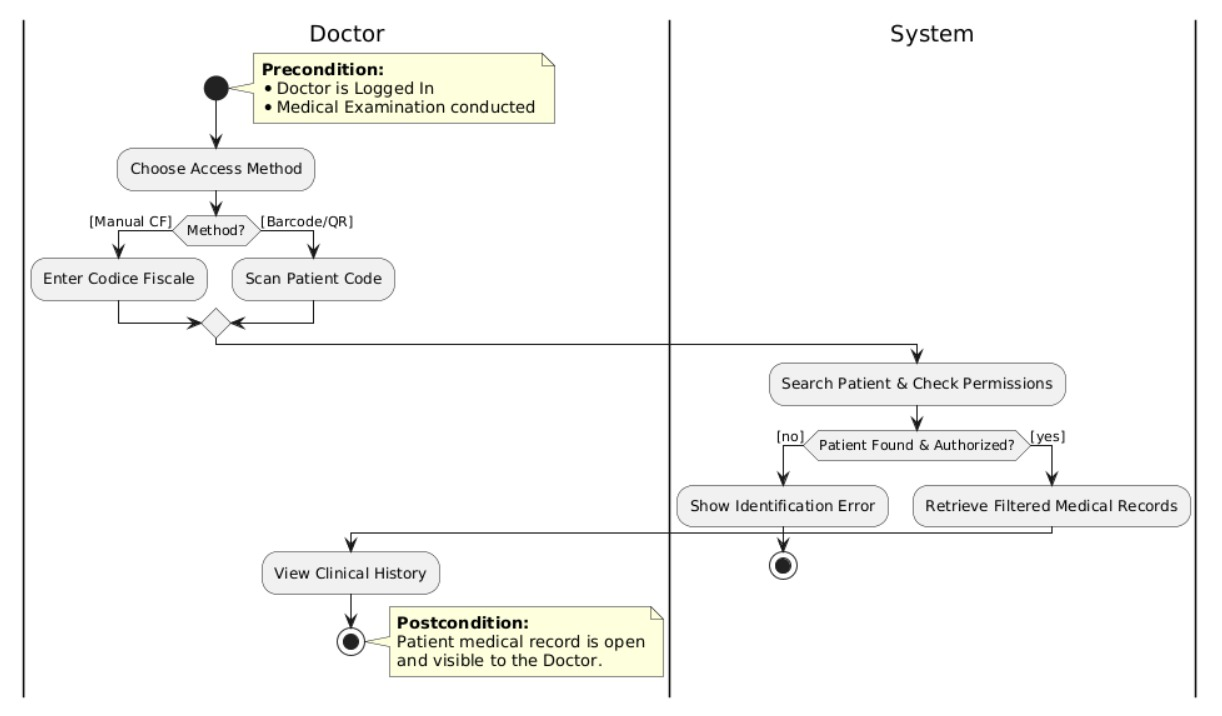
\includegraphics[width=0.8\textwidth]{Activity_Diagram/DoctorMedicalRecord.jpeg}
        \captionof{figure}{Activity Diagram regarding Doctor Accessing Patient's Medical Record}
    \end{center}

    \textbf{Using:} 
    
    \begin{itemize}
        \item \textbf{UC42} Medical record access (Doctor) ,
    \end{itemize}
\end{minipage}
\vspace{3em}

\begin{ucedits}
Following review of D2 the activity diagram number 6 was split to better reflect use cases.
\end{ucedits}



\phantomsection
\begin{minipage}{\textwidth}
    \phantomsection
    \subsection{Activity Diagram 6.2. Doctor uploads Prescription / Exemption / Examination}
    The following activity diagram shows the entire flow of uploading a prescription, exemption, or examination from the doctor's perspective.
    \begin{center}
        
\includegraphics[width=0.8\textwidth]{Activity_Diagram/DoctorUploads.jpeg}
        \captionof{figure}{Activity Diagram regarding Doctor Uploading Prescription / Exemption / Examination}
    \end{center}

    \textbf{Using:} 

    \begin{itemize}
        \item \textbf{UC3} Create Prescription / Exemption,
        \item \textbf{UC4} Upload Examination,    
    \end{itemize}

    
\end{minipage}
\vspace{3em}

\begin{ucedits}
Following review of D2 the activity diagram number 6 was split to better reflect use cases.
\end{ucedits}


\phantomsection
\begin{minipage}{\textwidth}
    \subsection{Activity Diagram 8. Patient Cancel and reschedule appointment}
    The following activity diagram shows the entire flow of cancellation and rescheduling of an appointment from the patient's perspective.
    \begin{center}
        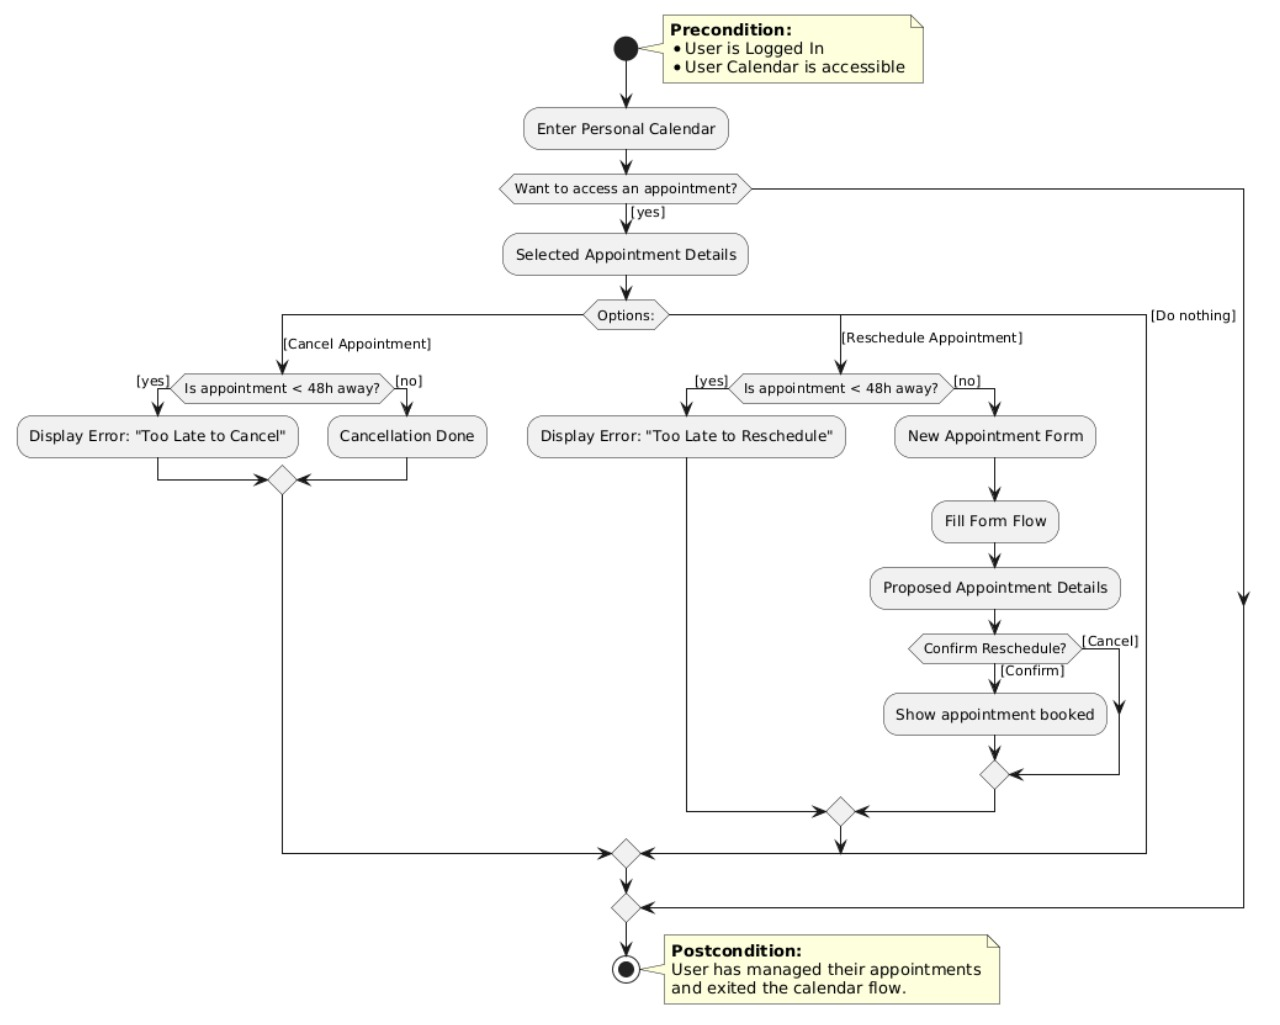
\includegraphics[width=0.8\textwidth]{Activity_Diagram/PatientCancelReschedule.jpeg}
        \captionof{figure}{Activity Diagram regarding Patient Cancel and reschedule appointment}
    \end{center}
    
    \textbf{Using:} 

    \begin{itemize}
        \item \textbf{UC10} Cancel Appointment (Patient),
        \item \textbf{UC29} Appointment rescheduling,
    \end{itemize}
\end{minipage}
\vspace{3em}

\begin{ucedits}
Following review of D2 this activity diagram was added to visualize the steps of the respective use cases.
\end{ucedits}

\phantomsection
\begin{minipage}{\textwidth}
    \subsection{Activity Diagram 9. Patient Medical record and Prescriptions consultation}
    The following activity diagram shows the entire flow of patient medical record access and prescription consultation.
    \begin{center}
        
\includegraphics[width=0.8\textwidth]{Activity_Diagram/PatientMedicalRecordPrescriptions.jpeg}
        \captionof{figure}{Activity Diagram regarding Patient Medical record and Prescriptions consultation}
    \end{center}
    
    \textbf{Using:} 
    
    \begin{itemize}
        \item \textbf{UC38} Prescription Consultation,
        \item \textbf{UC39} Detailed Prescription Access,    
        \item \textbf{UC40} Medical Record Access,    
    \end{itemize}
    
\end{minipage}
\vspace{3em}

\begin{ucedits}
Following review of D2 this activity diagram was added to visualize the steps of the respective use cases.
\end{ucedits}\

\phantomsection
\subsection{Class Diagram}
The following screenshots present the updated class diagram, organized into logical groups 
based on their relevance to the user flows described in the following sections. Each group highlights a meaningful 
subset of the system's classes and their relationships, rather than representing the diagram 
in its entirety. This grouping aims to improve clarity and readability, making it easier to 
trace the connection between each user flow and the classes involved.
\begin{center}
    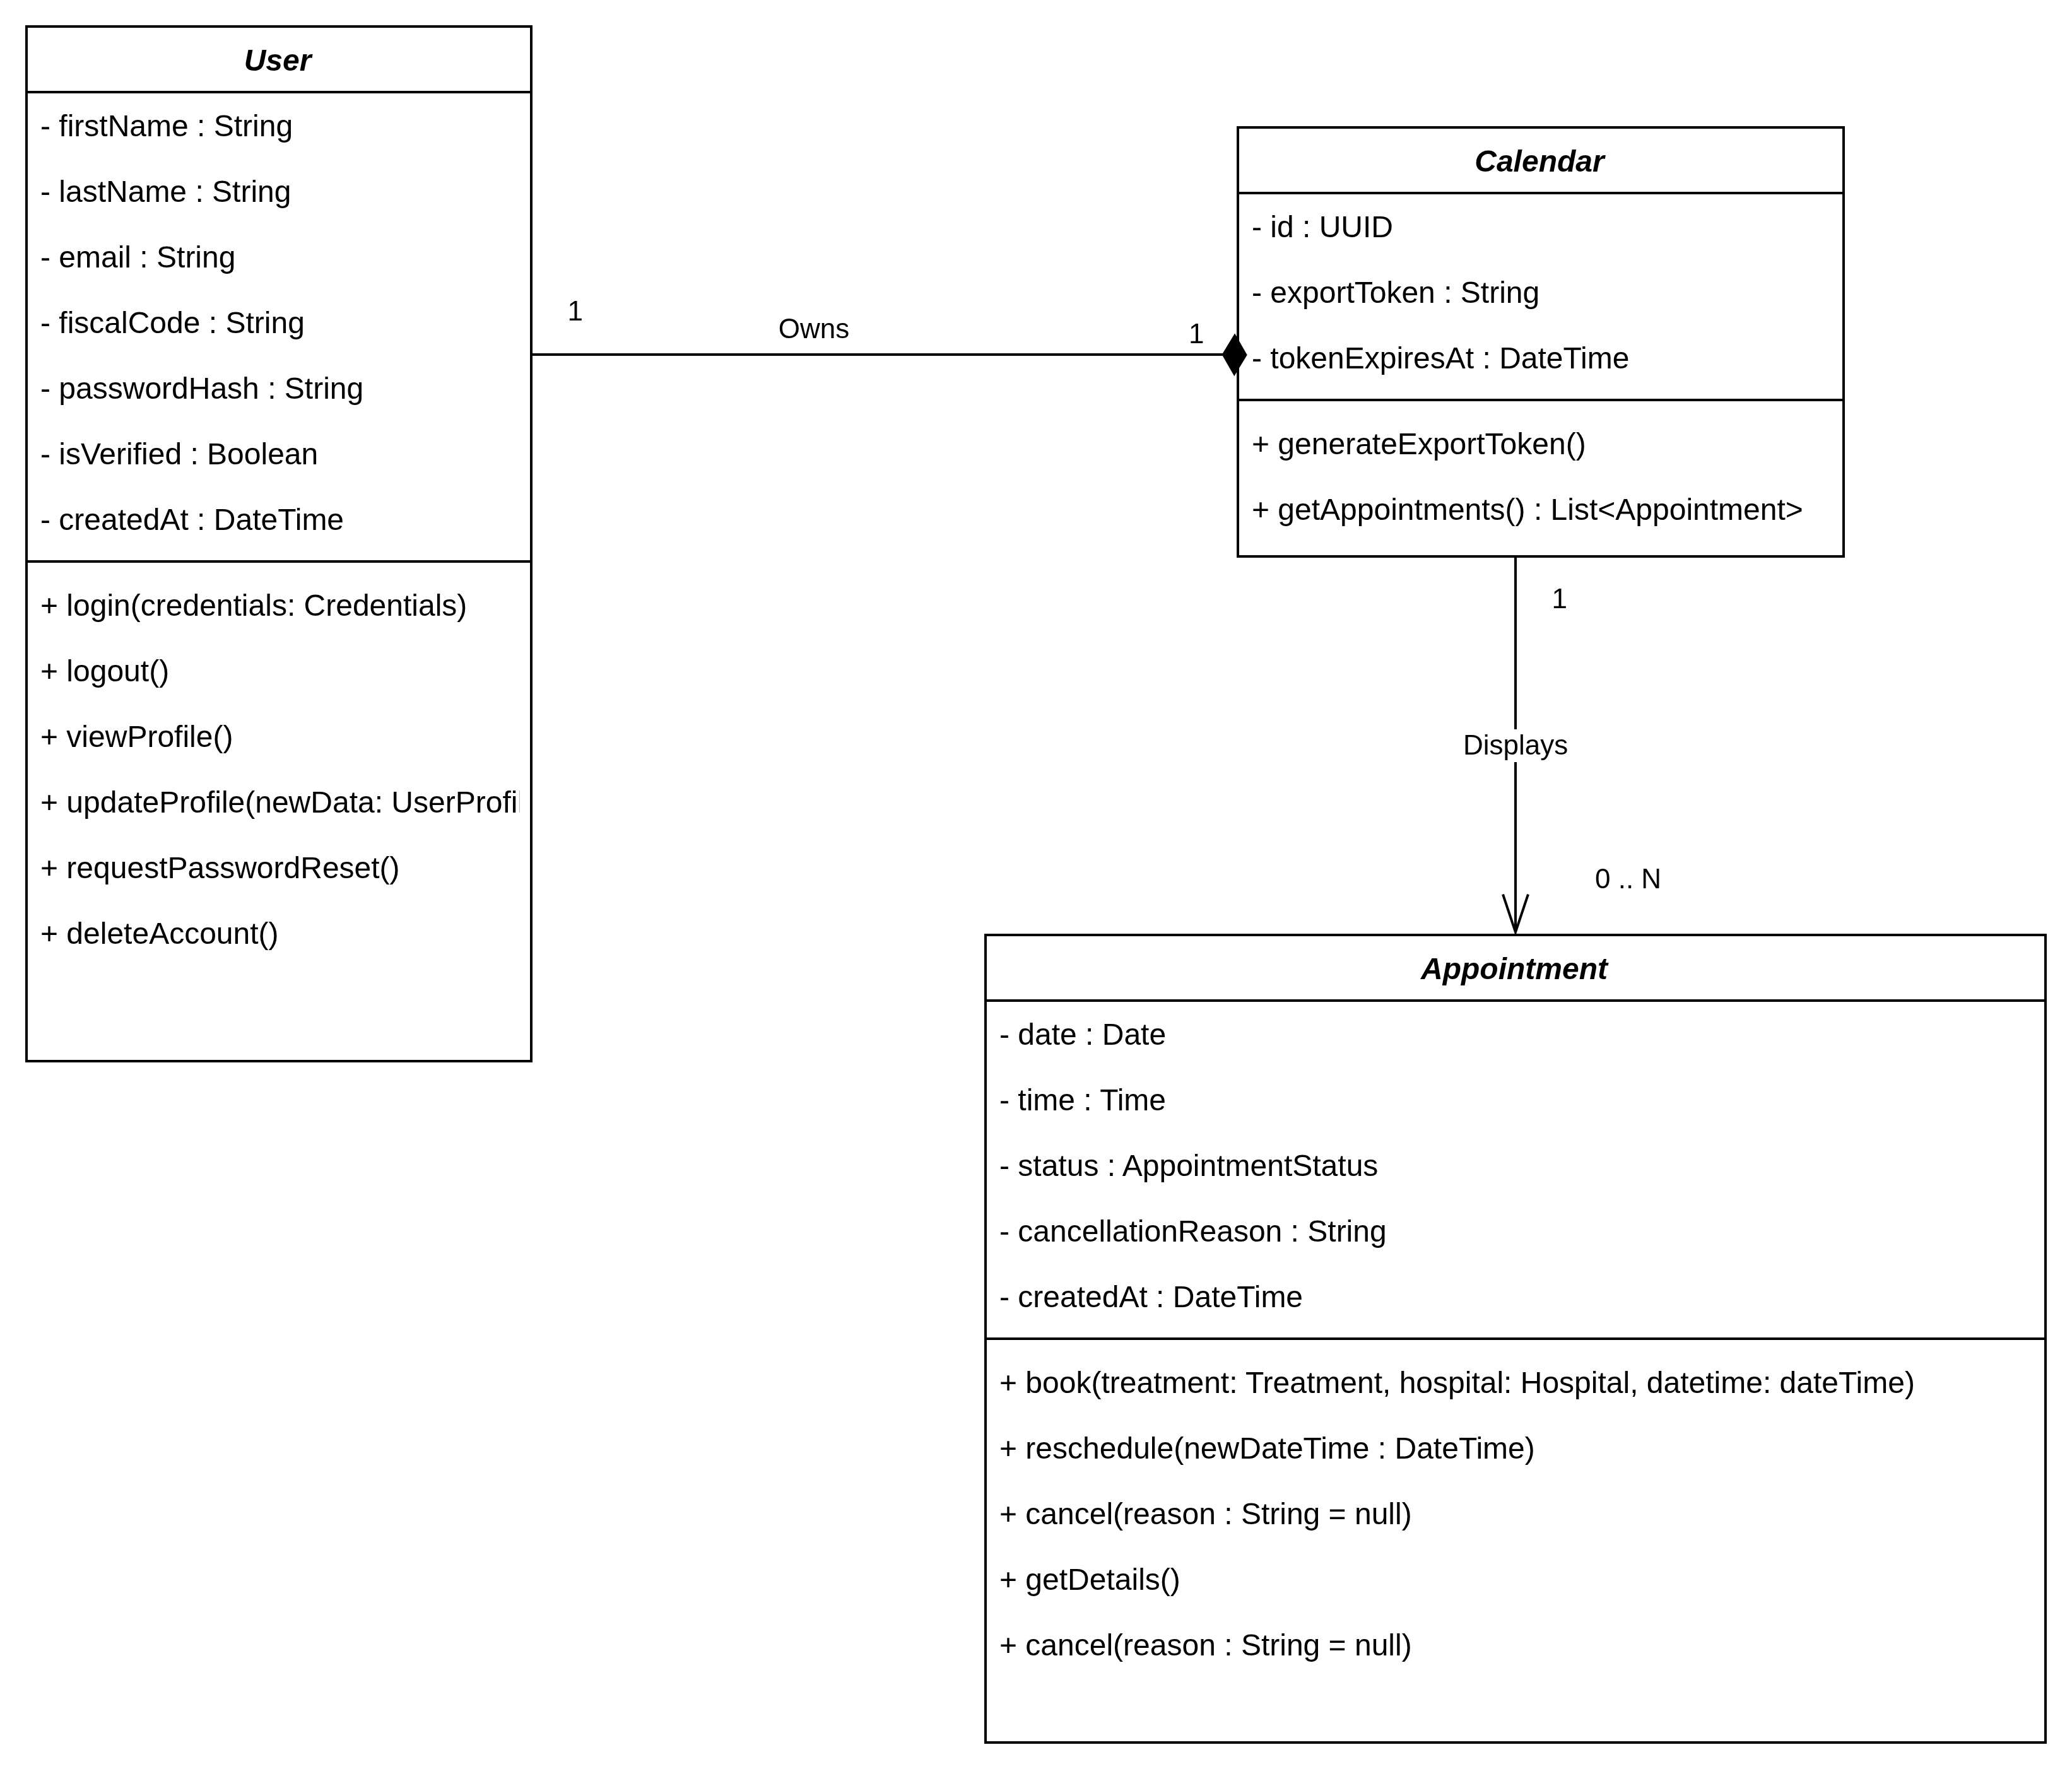
\includegraphics[width=0.9\textwidth, height=0.75\textheight, keepaspectratio]{Class_Diagram/review/genericUser.png}
    \captionof{figure}{Class diagram — Generic User}
\end{center}

\vspace{2em}

\begin{center}
    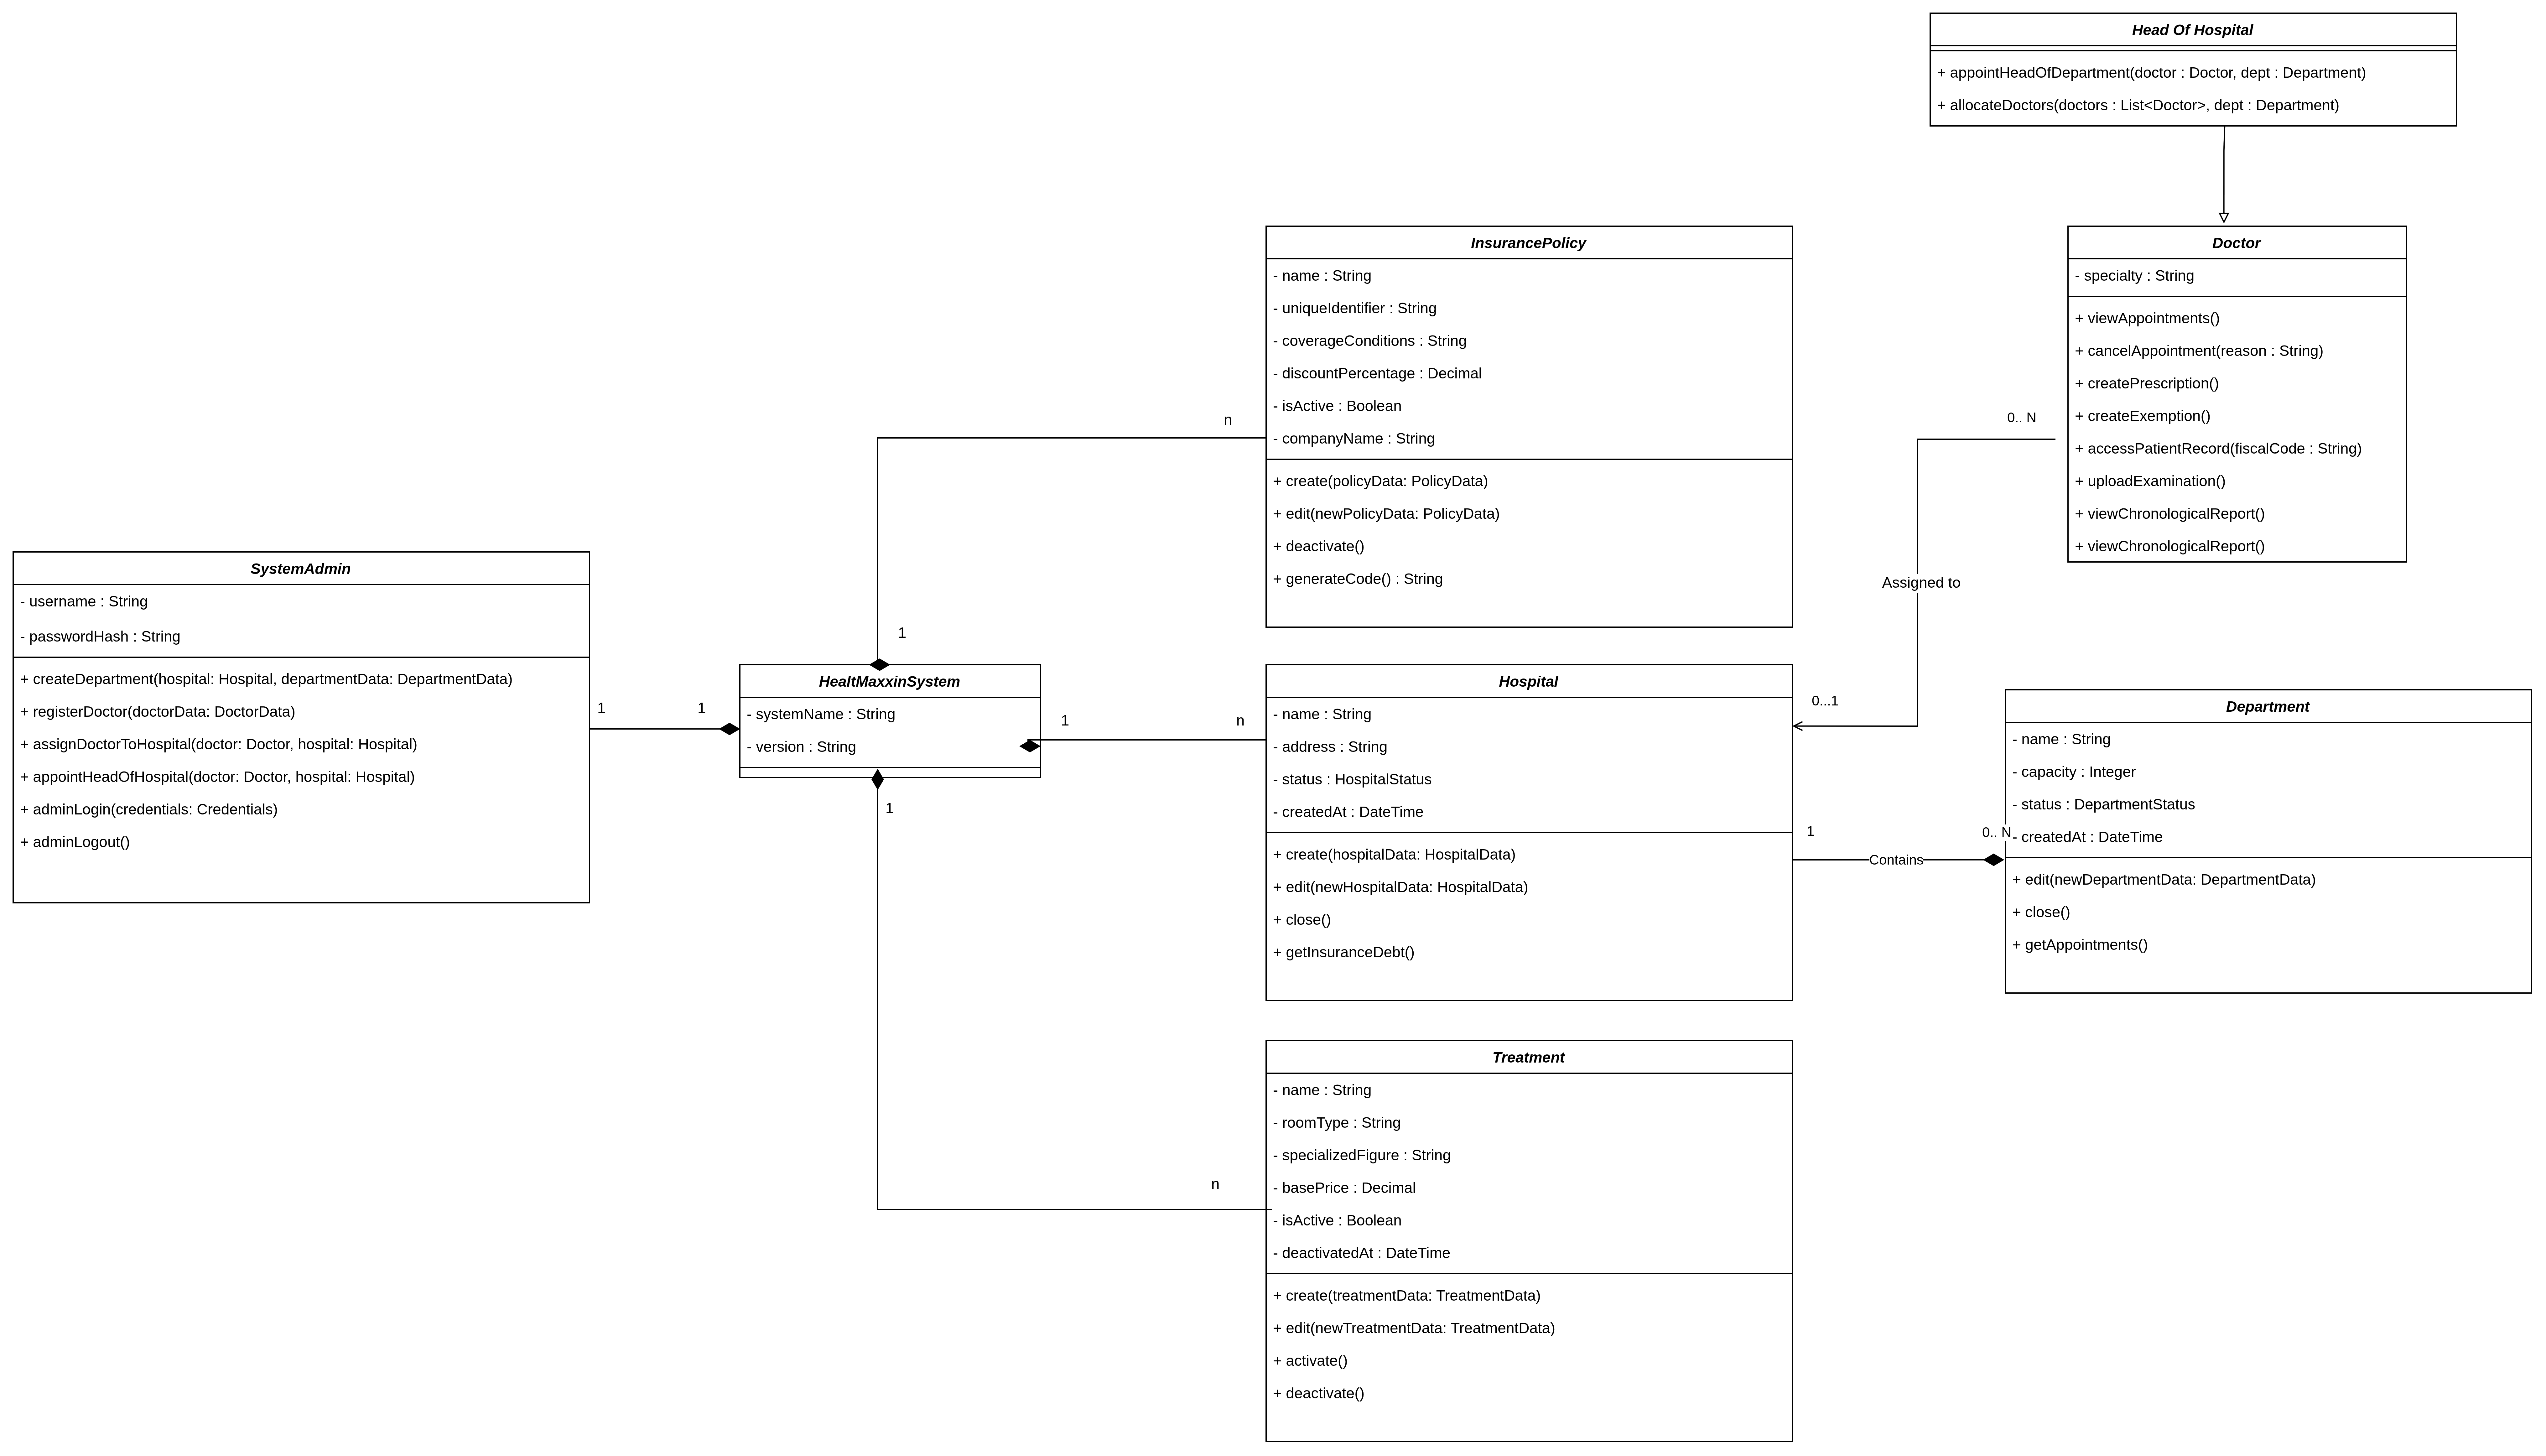
\includegraphics[width=0.9\textwidth, height=0.75\textheight, keepaspectratio]{Class_Diagram/review/admin.png}
    \captionof{figure}{Class diagram — Admin}
\end{center}

\vspace{3em}
\begin{center}
    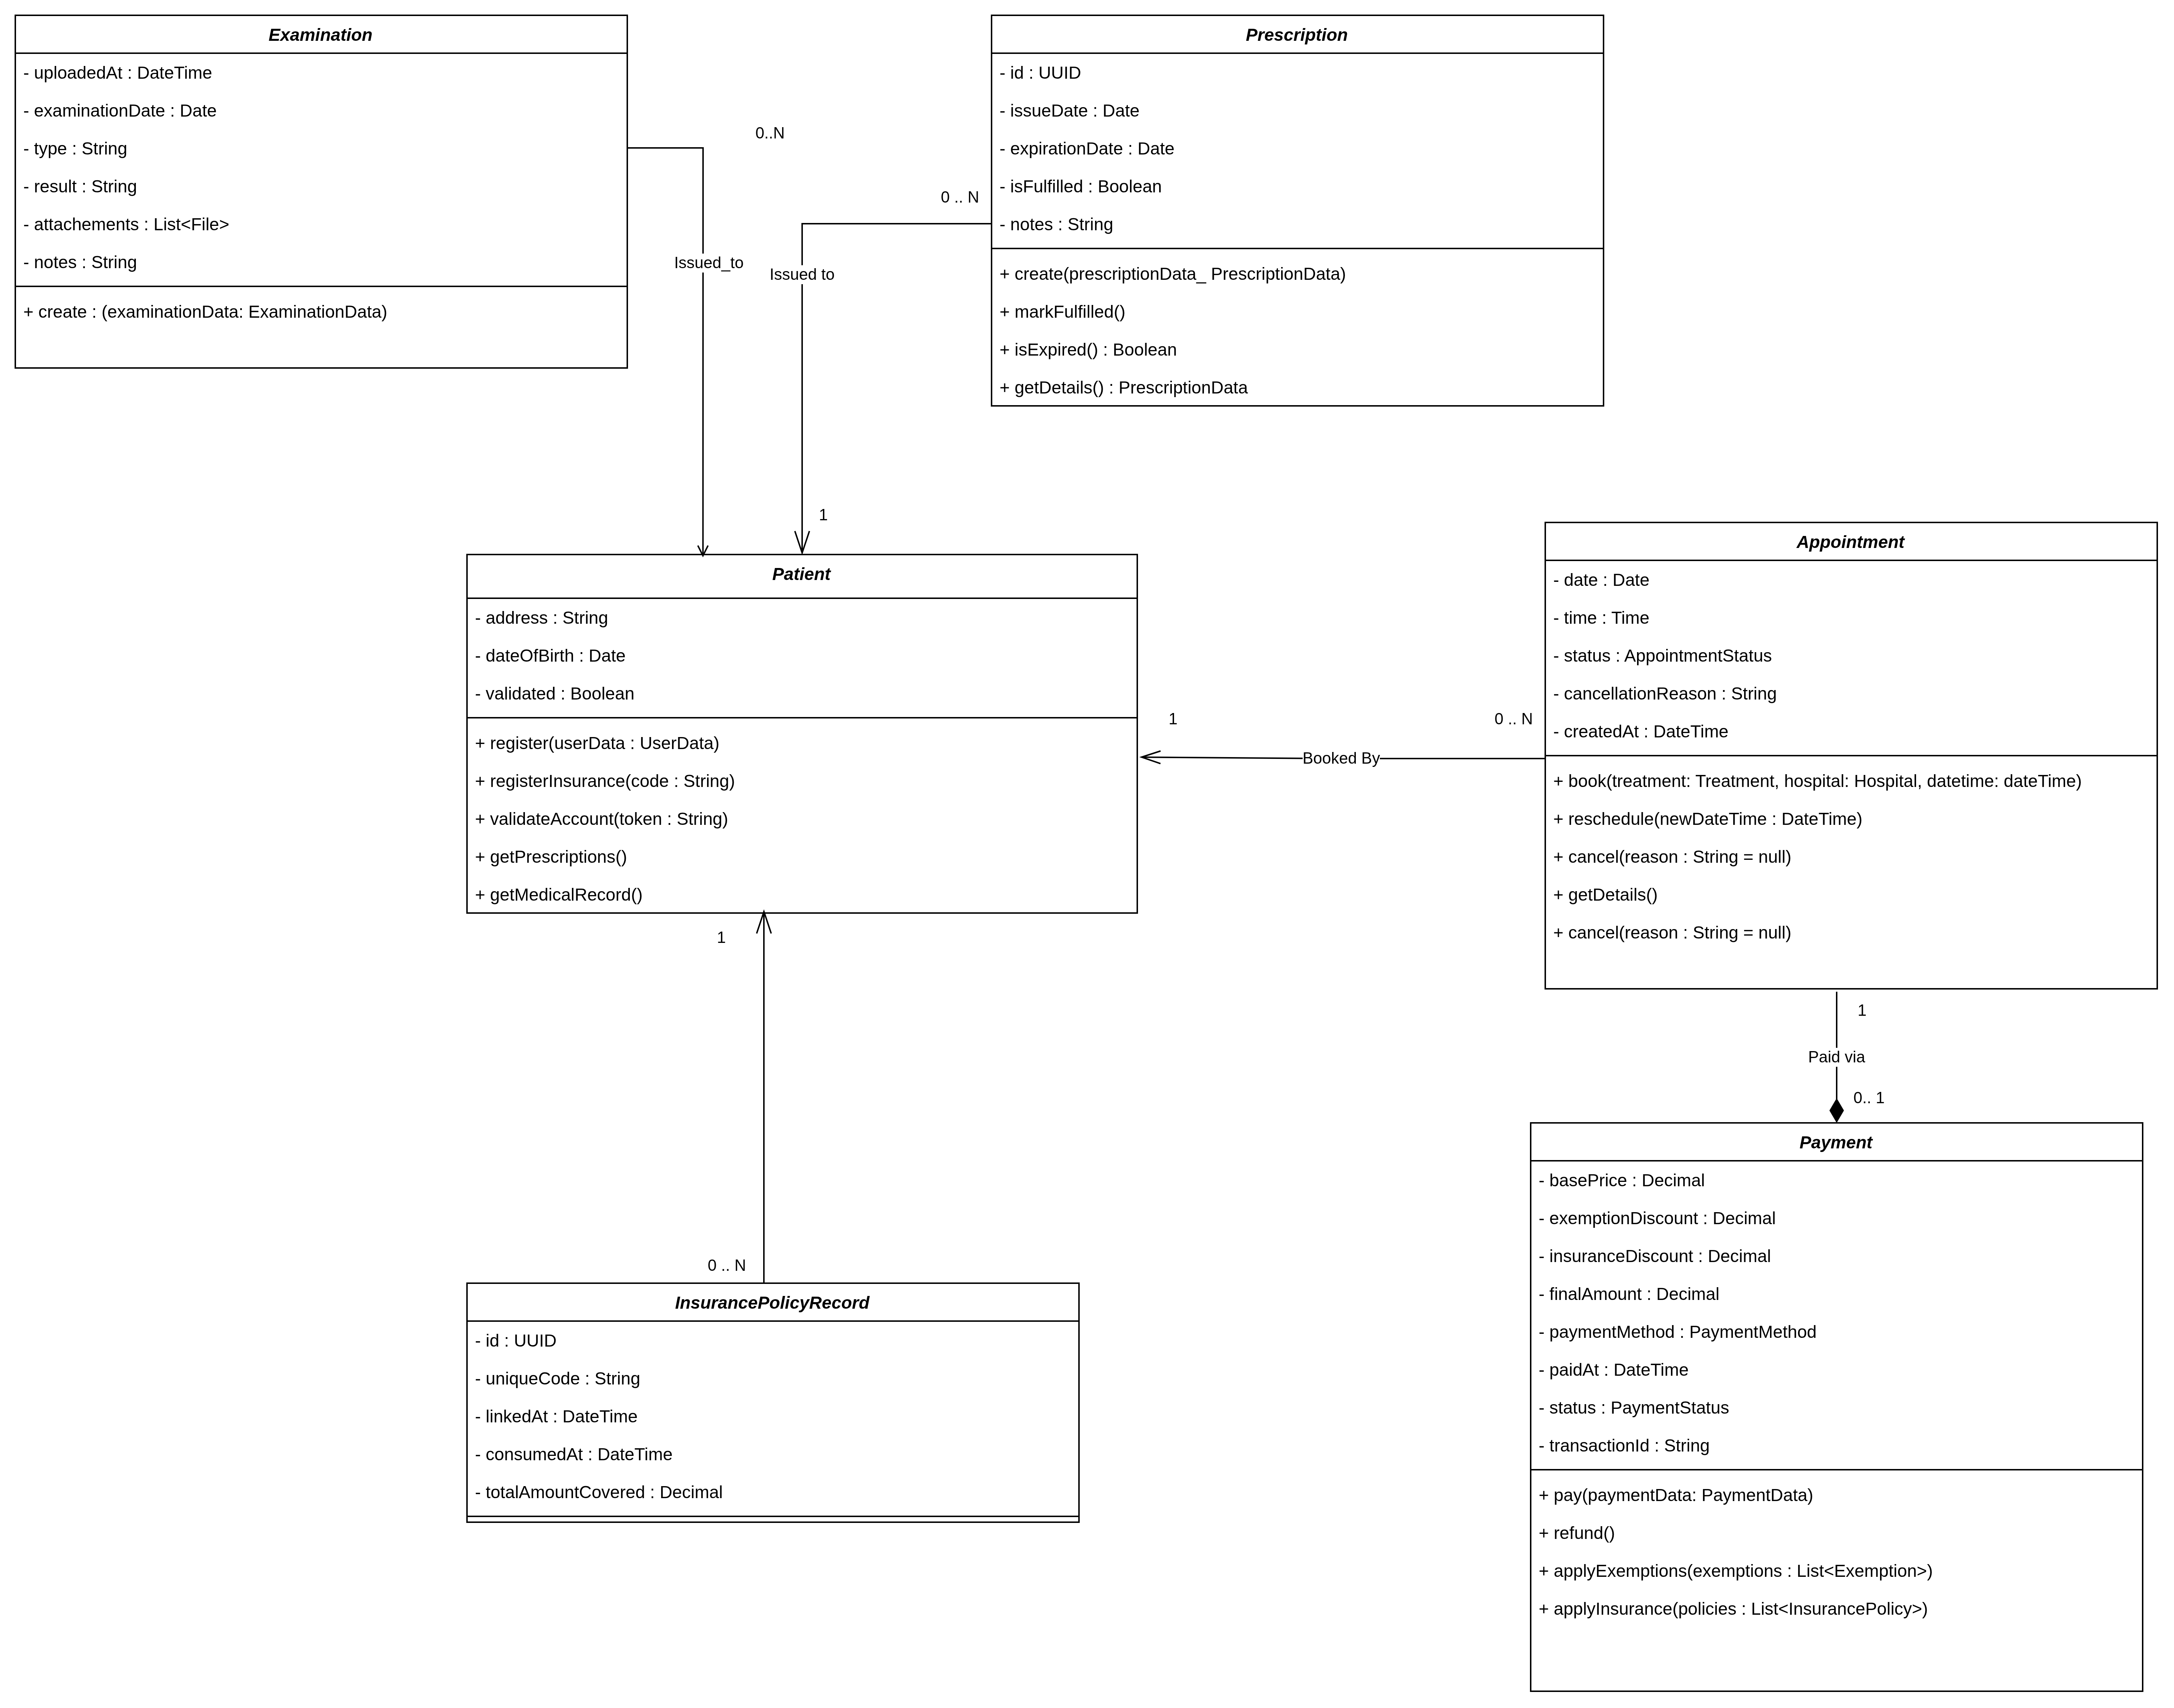
\includegraphics[width=0.9\textwidth, height=0.75\textheight, keepaspectratio]{Class_Diagram/review/patient.png}
    \captionof{figure}{Class diagram — Patient}
\end{center}

\vspace{3em}

\begin{center}
    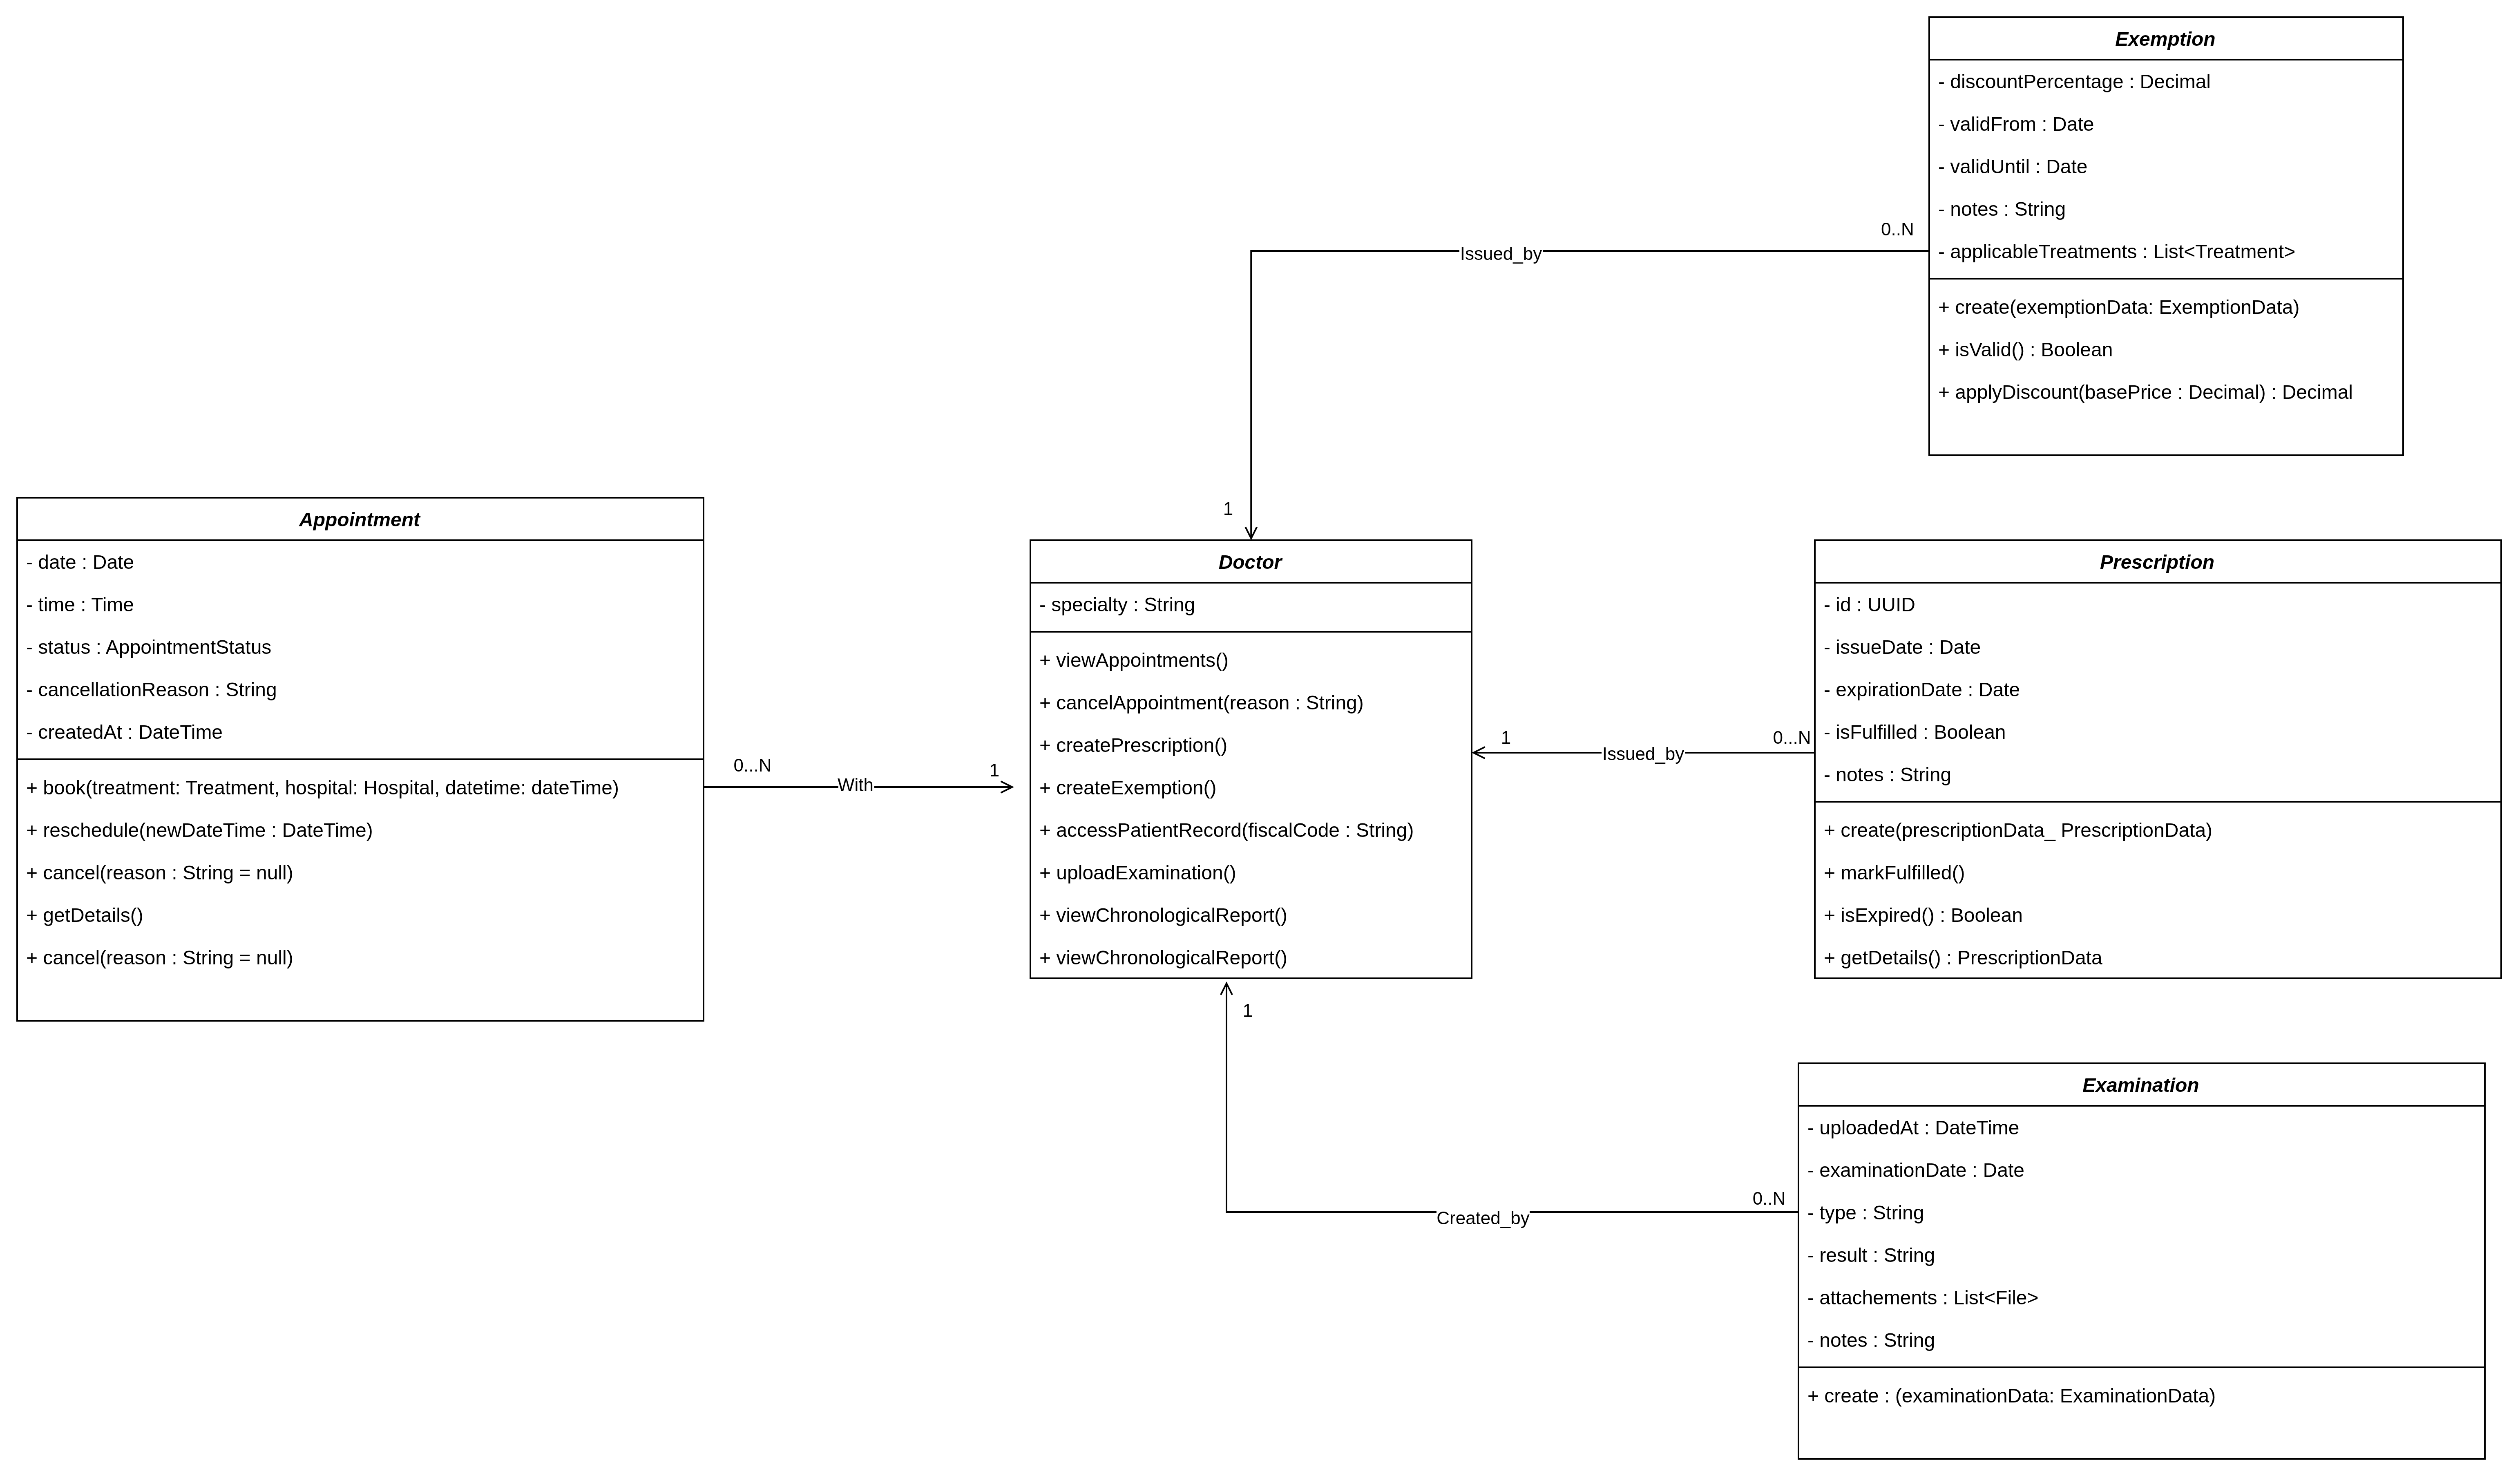
\includegraphics[width=0.9\textwidth, height=0.75\textheight, keepaspectratio]{Class_Diagram/review/doctor.png}
    \captionof{figure}{Class diagram — Doctor}
\end{center}
\begin{center}
    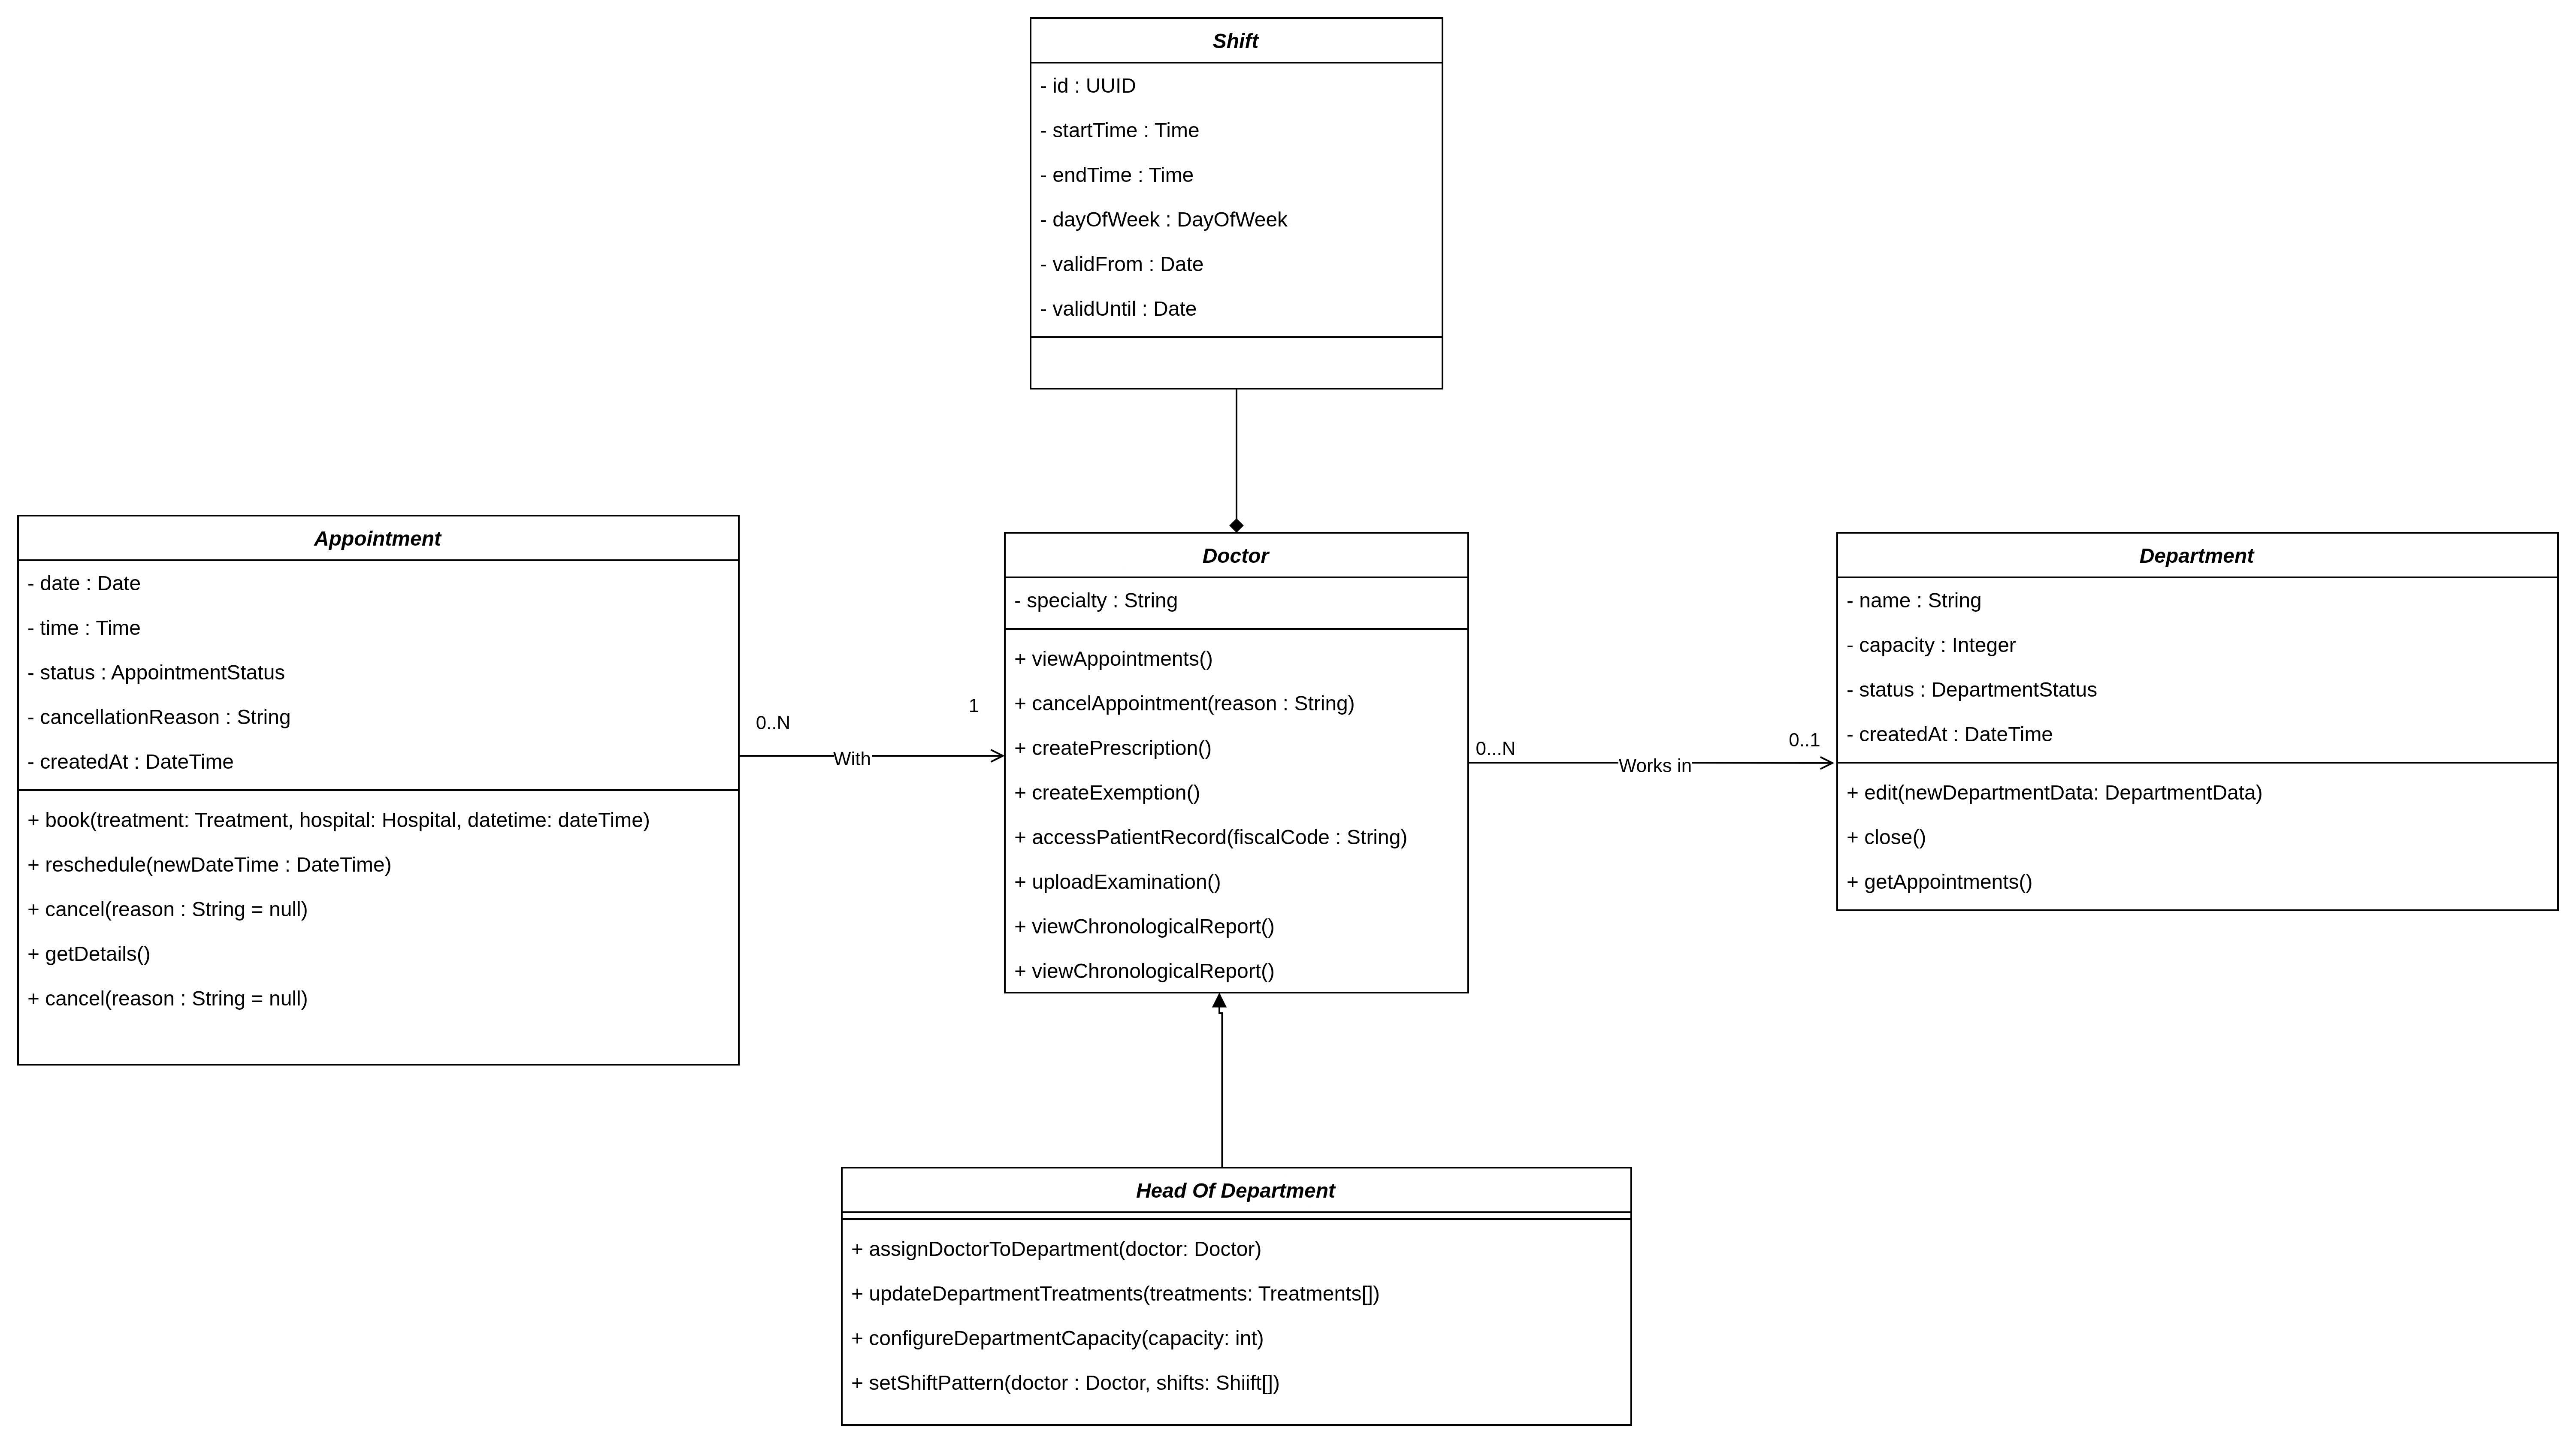
\includegraphics[width=0.9\textwidth, height=0.75\textheight, keepaspectratio]{Class_Diagram/review/headOfDepartment.png}
    \captionof{figure}{Class diagram — Head of Department}
\end{center}
\begin{center}
    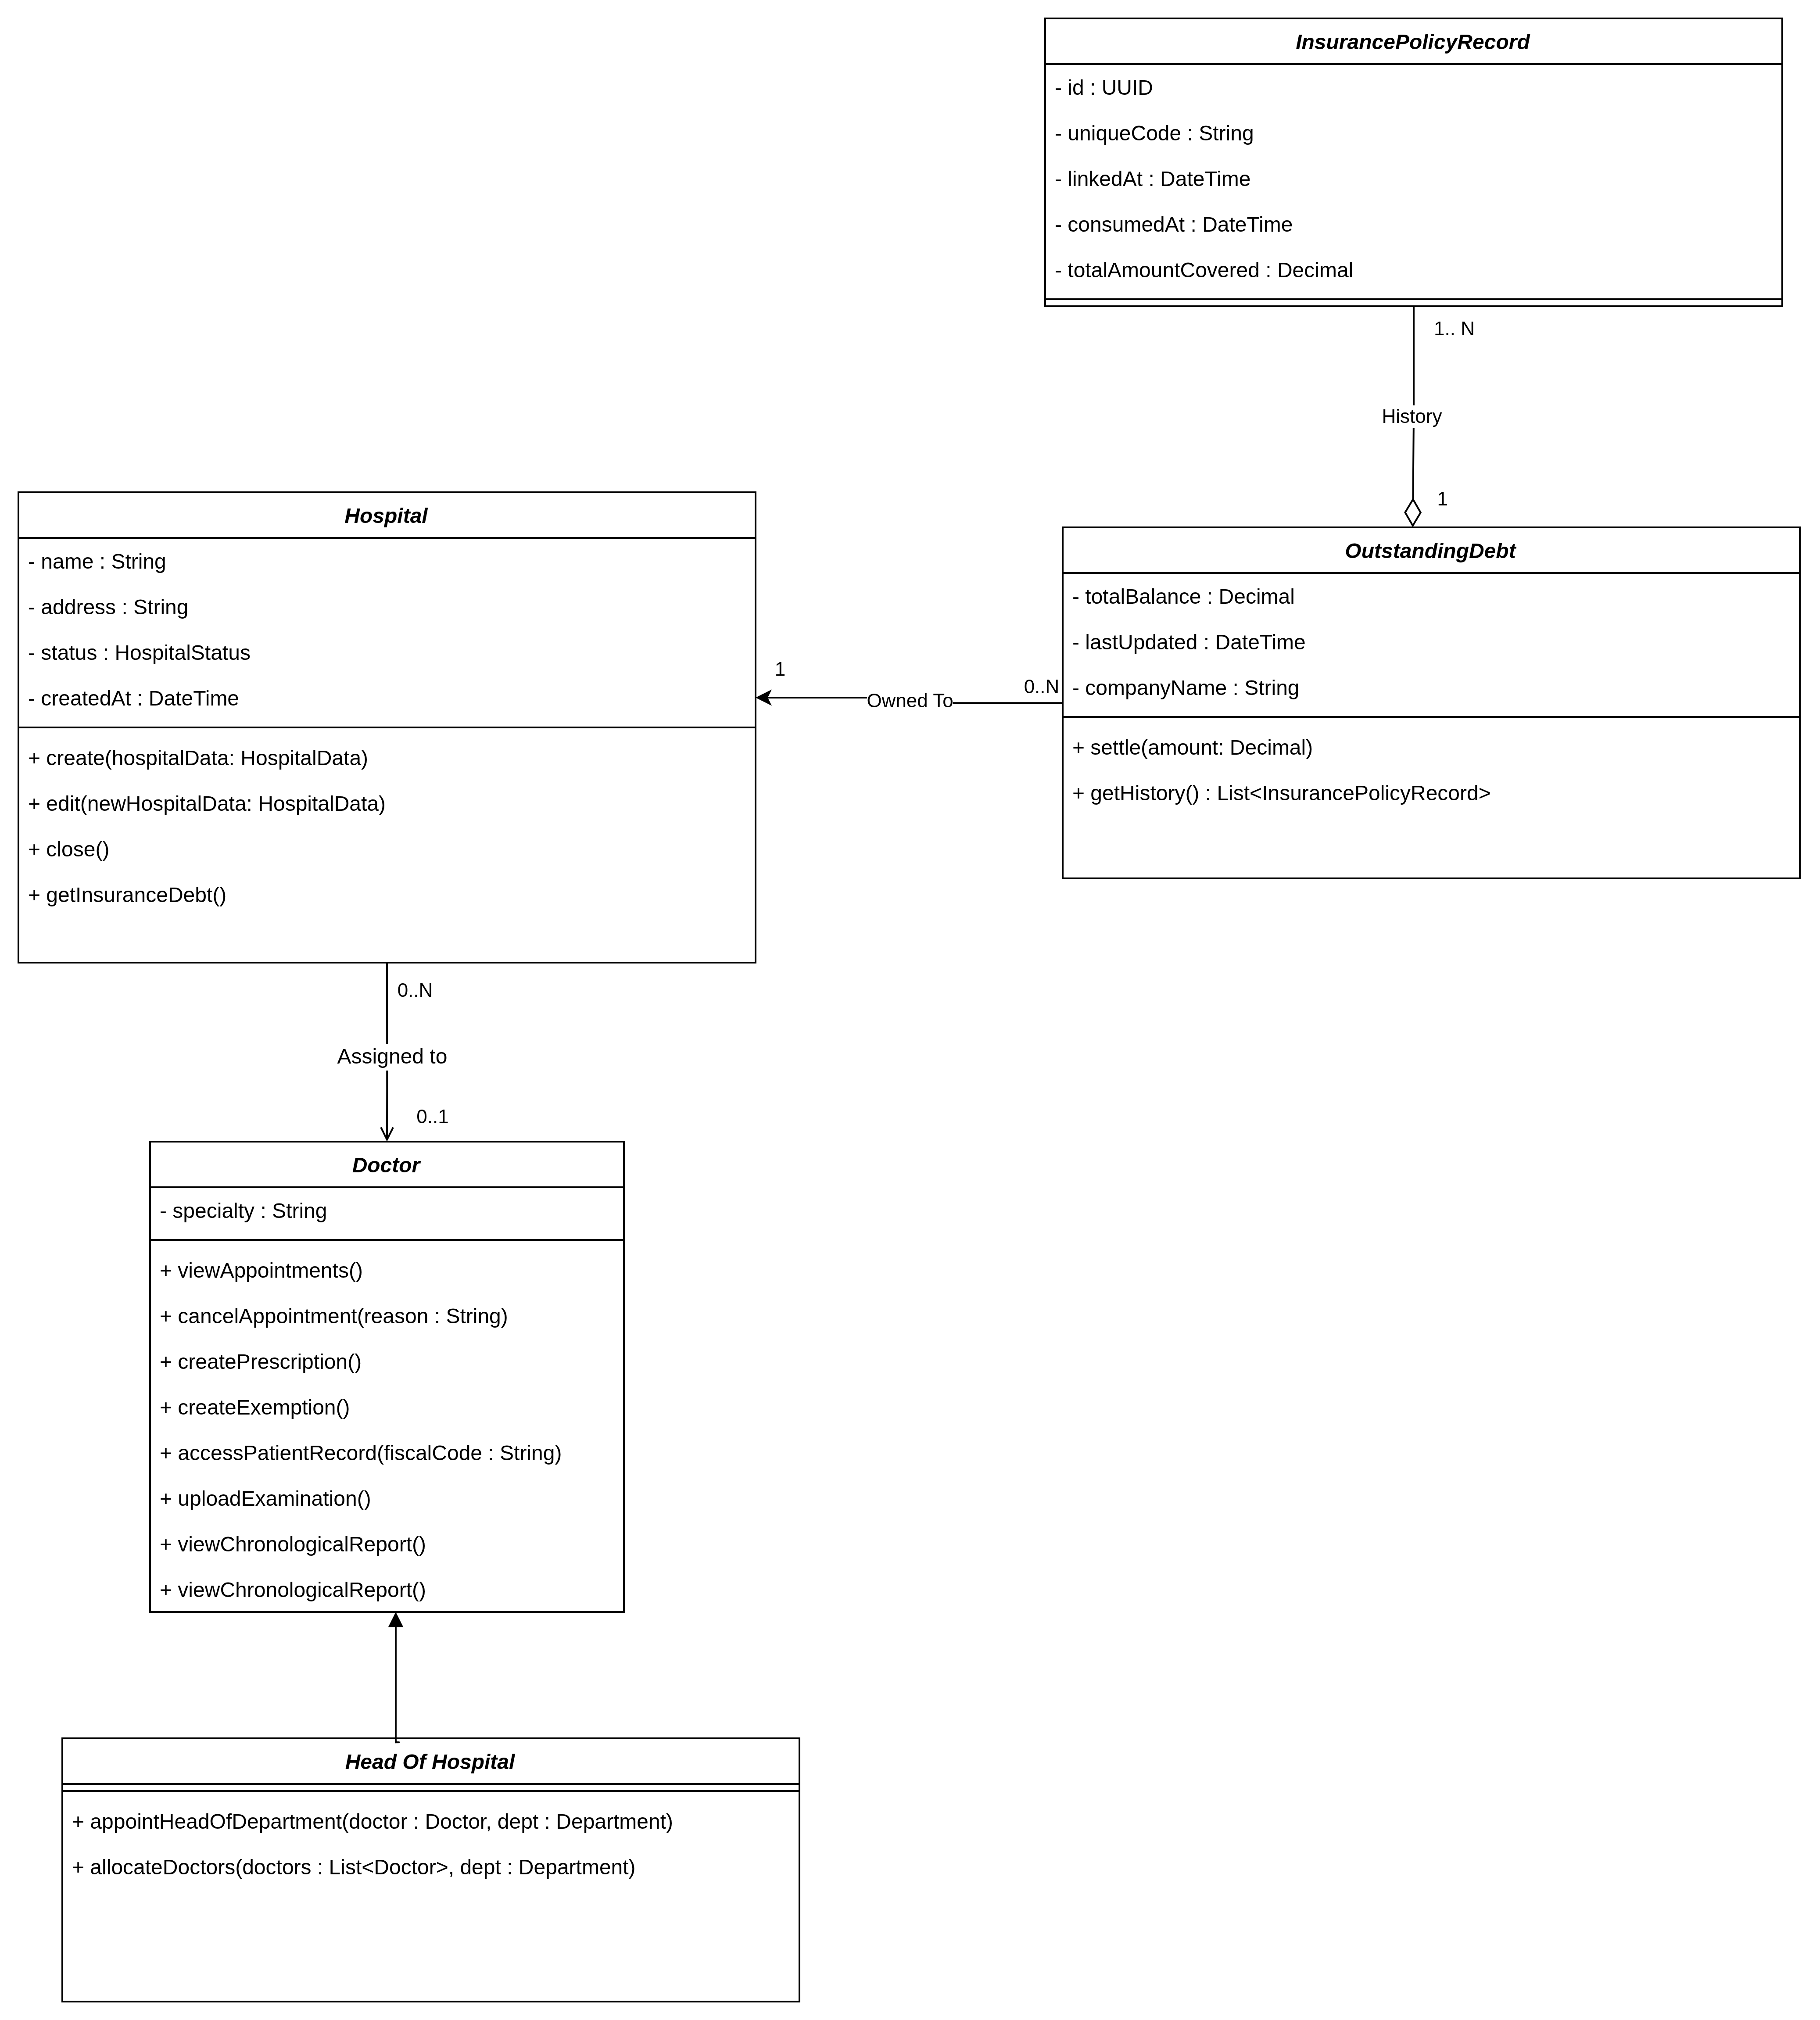
\includegraphics[width=0.9\textwidth, height=0.75\textheight, keepaspectratio]{Class_Diagram/review/headOfHospital.png}
    \captionof{figure}{Class diagram — Head of Hospital}
\end{center}



\vspace{3em}




\section{Context Description}

\subsection{General Overview}
This project involves the design of an extensive and centralized software application, intended for use in the administration of the operations of a network of private healthcare services spread over the Italian territory. This application, operating exclusively on an outpatient and ambulatory model, seeks to digitalize key administrative operations, thereby optimizing the entire experience for all relevant stakeholders involved in the healthcare sector.

At the heart of this application is the ``Examination,'' defined as a specific, scheduled transaction between a patient and a doctor. In order to support this model, the application will offer medical professionals tools for scheduling, administrators an extensive toolset for overseeing hospital operations, and patients an optimized interface for scheduling examinations and processing transactions.

The specific features and step-by-step operations for each of these stakeholders will be discussed in the objectives and requirements sections of the application.

\subsection{System Boundaries}
A major technical limit of this system is its ability to integrate with third-party insurance providers. The application will be unable to verify policies in real time, as it will not have access to any external, live databases from third-party insurance providers. The system will, therefore, rely on a simulated system for managing patient insurance information, with codes created internally. The process of reconciling insurance claims and outstanding debts owed to the hospital will, therefore, not be automated but will be internally simulated.

In addition, the fact that the platform has been specifically designed for the logistics of the scheduled outpatient examinations means that the current scope of the system has been specifically defined in terms of doctors, facility managers, and patients. There has been no specific design of the system in terms of dedicated interfaces and access levels for other professional figures in the hospital scenario, such as nurses, medical technicians, and administrative secretaries.
      
Furthermore, the administration of medications and pharmaceuticals is completely out of the scope of this project. The functionality of the application still remains completely focused on the administration and processing of medical consultations.
\newpage

\newpage
\phantomsection %% non so perché senza l'indice funziona male :///
% -------------------------------------------------------
\section{Architecture Choice and Language Used}
% -------------------------------------------------------
This section aims to provide a clear description of the architecture and language used in the developement of the HealthMaxxing app. Together with the reasons behind such choices.
\phantomsection 
\subsection{Architecture Type: 3-Tier Architecture}
\phantomsection 
\subsubsection{Description}

The application follows a \textbf{3-Tier Architecture} pattern, separating the system into three distinct layers:

\begin{itemize}
  \item \textbf{Presentation Layer (Frontend)} --- React with Vite
  \item \textbf{Business Logic / API Layer (Backend)} --- Django REST Framework
  \item \textbf{Data Layer (Database)} --- PostgreSQL
\end{itemize}
\phantomsection 
\subsubsection{Why 3-Tier?}

\begin{itemize}
  \item \textbf{Maintainability:} Each tier can be developed, tested, and maintained independently. Changes in one layer do not directly affect others.
  \item \textbf{Separation of Duties:} Clear separation between UI concerns, business logic, and data persistence. Frontend developers focus on UX, backend developers focus on APIs and business rules, and database administrators manage data integrity.
  \item \textbf{Scalability:} Each tier can be scaled independently based on demand. The frontend can be served via CDN, the API can be load-balanced, and the database can use replication.
  \item \textbf{Industry Standard:} 3-tier is the most widely adopted pattern in modern web development, making the codebase more familiar to new team members.
\end{itemize}

\phantomsection 
\subsubsection{Project Structure}

\textbf{Main folders and files:}

\begin{itemize}
    \item \textbf{backend/} --- Contains the Django REST Framework application, business logic, models, serializers, and API endpoints.
    
    \item \textbf{frontend/} --- Contains the React application, user interface components, routing, state management, and API integration.
    
    \item \textbf{nginx/} --- Configuration files for the Nginx reverse proxy.
    
    \item \textbf{docs/} --- Project documentation and supporting materials.
    
    \item \textbf{docker-compose.yml} --- Defines and orchestrates the multi-container application environment.
    
    \item \textbf{Dockerfile.devbox} --- Docker image configuration used during development.
    
    \item \textbf{requirements.txt} --- Python dependencies required by the backend.
    
    \item \textbf{package.json} --- JavaScript dependencies and scripts used by the frontend.
    
    \item \textbf{README.md} --- General project documentation and setup instructions.

    \begin{figure}[htbp]
      \centering
      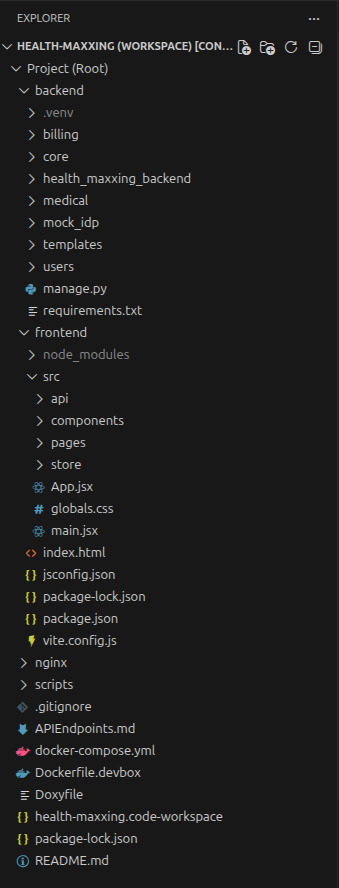
\includegraphics[width=0.35\textwidth]{ScreenshotD3/FoldStruct.jpeg}
      \caption{Project structure}
      \label{fig:folder-structure}
    \end{figure}
    \FloatBarrier

\end{itemize}
\phantomsection 
% -------------------------------------------------------
\subsection{Language Used and Why}
% -------------------------------------------------------
\phantomsection 
\subsubsection{Frontend Language: JavaScript (React 18.3.1)}

\textbf{Why React?}

\begin{itemize}
  \item \textbf{Reusable Components:} React's component-based architecture allows building modular, reusable UI pieces that reduce code duplication.
  \item \textbf{Flexibility for Routing:} React Router DOM enables client-side routing, allowing seamless navigation without full page reloads.
  \item \textbf{Security Measures:} React provides built-in protections against common vulnerabilities like XSS attacks through automatic escaping.
  \item \textbf{Large Ecosystem:} Extensive community support, libraries, and tools available.
  \item \textbf{Developer Experience:} JSX syntax makes code more readable and maintainable.
\end{itemize}

\textbf{Why NOT Plain HTML/CSS?}

\begin{itemize}
  \item Plain HTML/CSS is considered outdated for modern web applications and not an industry standard.
  \item Lacks dynamic interactivity without extensive custom JavaScript.
  \item No component reusability or state management capabilities.
  \item Poor performance with complex UIs.
\end{itemize}
\phantomsection 
\subsubsection{Backend Language: Python (Django 4.2.30)}

\textbf{Why Django?}

\begin{itemize}
  \item Included as the framework of choice for this project.
  \item Excellent for rapid API development with built-in authentication, ORM, and admin panel.
  \item Strong security features (CSRF protection, SQL injection prevention, etc.).
  \item Well-documented and widely used in production environments.
\end{itemize}
\phantomsection 
% -------------------------------------------------------
\subsection{Database: PostgreSQL}
% -------------------------------------------------------
\phantomsection 
\subsubsection{Why PostgreSQL?}

\begin{itemize}
  \item \textbf{Team Familiarity:} All team members are comfortable with PostgreSQL and the relational database paradigm.
  \item \textbf{Industry Standard:} PostgreSQL is a robust, production-ready relational database trusted by many organizations.
  \item \textbf{Strong Consistency:} ACID compliance ensures data integrity.
  \item \textbf{Advanced Features:} Supports JSON, full-text search, and complex queries out of the box.
\end{itemize}
\phantomsection 
\subsubsection{ER Diagram}

\begin{figure}[htbp]
    \centering
    \includegraphics[width=\textwidth]{ScreenshotD3/ER.png} % Scales to exactly 100% of text width
    \caption{ER diagram}
    \label{fig:large_image}
\end{figure}

\FloatBarrier
\phantomsection 
\subsubsection{Example of some Tables}

\begin{figure}[htbp]
        \centering
        \begin{subfigure}[b]{0.47\textwidth}
            \centering
            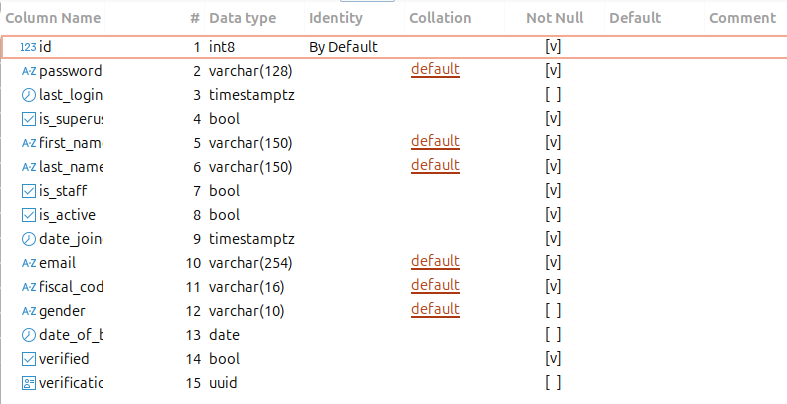
\includegraphics[width=\linewidth]{ScreenshotD3/tableUser.png}
            \caption{}
            \label{User Table}
        \end{subfigure}
        \hfill \begin{subfigure}[b]{0.47\textwidth}
            \centering
            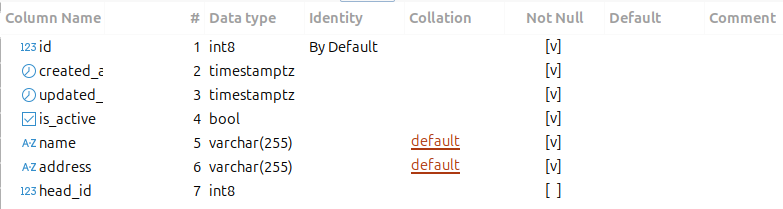
\includegraphics[width=\linewidth]{ScreenshotD3/tableHospital.png}
            \caption{}
            \label{Hospital Table}
        \end{subfigure}
        
        \caption{table of users (a), table of hospitals (b)}
        \label{User and Hospital Tables}
\end{figure}
\FloatBarrier

\phantomsection 
% -------------------------------------------------------
\subsection{Dependencies}
% -------------------------------------------------------
\phantomsection 
\subsubsection{Backend Dependencies}

\begin{longtable}{L{3.6cm} C{2.0cm} L{8.8cm}}
  \rowcolor{tableheader}
  \color{white}\bfseries Dependency &
  \color{white}\bfseries Version &
  \color{white}\bfseries Purpose \\
  \endfirsthead
  \rowcolor{tableheader}
  \color{white}\bfseries Dependency &
  \color{white}\bfseries Version &
  \color{white}\bfseries Purpose \\
  \endhead
  Django & 4.2.30 & Core web framework used to build the backend application and REST API \\
  \rowcolor{tablerowalt}
  Django REST Framework & 3.17.1 & Provides tools for building RESTful APIs, including serialization, authentication, and viewsets \\
  django-admin-confirm & 1.0.1 & Adds confirmation steps to Django admin actions to prevent accidental bulk operations \\
  \rowcolor{tablerowalt}
  django-cors-headers & 4.9.0 & Handles Cross-Origin Resource Sharing (CORS) between frontend and backend services \\
  djangorestframework-simplejwt & 5.5.1 & Implements JWT-based authentication for Django REST Framework \\
  \rowcolor{tablerowalt}
  psycopg & 3.3.4 & PostgreSQL database adapter for Python \\
  psycopg-binary & 3.3.4 & Pre-compiled PostgreSQL adapter for simplified installation and development \\
  \rowcolor{tablerowalt}
  ruff & 0.15.14 & Python linter and formatter used to enforce code quality standards \\
  asgiref & 3.11.1 & ASGI utilities providing asynchronous support required by Django \\
  \rowcolor{tablerowalt}
  sqlparse & 0.5.5 & SQL parsing library used internally by Django \\
  typing\_extensions & 4.15.0 & Backported and experimental type hinting features for Python \\
  \rowcolor{tablerowalt}
  tzdata & 2026.2 & Time zone database used for accurate date and time handling \\
  PyJWT & 2.13.0 & Creates, signs, decodes, and validates JSON Web Tokens \\
\end{longtable}
\phantomsection 
\subsubsection{Frontend Dependencies}

\begin{longtable}{L{3.6cm} C{2.0cm} L{8.8cm}}
  \rowcolor{tableheader}
  \color{white}\bfseries Dependency &
  \color{white}\bfseries Version &
  \color{white}\bfseries Purpose \\
  \endfirsthead
  \rowcolor{tableheader}
  \color{white}\bfseries Dependency &
  \color{white}\bfseries Version &
  \color{white}\bfseries Purpose \\
  \endhead
  React & 18.3.1 & Core UI library for building interactive components \\
  \rowcolor{tablerowalt}
  react-dom & 18.3.1 & Renders React components to the DOM \\
  react-router-dom & 6.0.0 & Client-side routing for seamless page navigation \\
  \rowcolor{tablerowalt}
  react-big-calendar & 1.20.0 & Feature-rich calendar component for displaying and managing scheduled events \\
  Vite & 5.4.1 & Lightning-fast build tool and dev server (modern webpack alternative) \\
  \rowcolor{tablerowalt}
  @vitejs/plugin-react & 4.3.1 & Vite plugin for React support with Fast Refresh \\
  axios & 1.17.0 & Promise-based HTTP client for making API requests from the frontend \\
  \rowcolor{tablerowalt}
  date-fns & 4.4.0 & Lightweight utility library for parsing, formatting, and manipulating dates \\
  zustand & 5.0.14 & Lightweight state management library for global application state, including authentication data \\
  \rowcolor{tablerowalt}
  jwt-decode & 4.0.0 & Decodes JWT tokens on the client side to extract user information and token claims without server requests \\
\end{longtable}
\phantomsection 
\subsubsection{Infrastructure Dependencies}

\begin{longtable}{L{3.6cm} L{10.8cm}}
  \rowcolor{tableheader}
  \color{white}\bfseries Dependency &
  \color{white}\bfseries Purpose \\
  \endfirsthead
  \rowcolor{tableheader}
  \color{white}\bfseries Dependency &
  \color{white}\bfseries Purpose \\
  \endhead
  Nginx & Reverse proxy server for routing requests, serving static assets, and load balancing \\
  \rowcolor{tablerowalt}
  Docker & Containerization platform for consistent development, testing, and production environments \\
  docker-compose & Orchestrates multi-container Docker applications (frontend, backend, database) \\
\end{longtable}

\textbf{Why These Infrastructure Tools?}

\begin{itemize}
  \item \textbf{Nginx:} Acts as a reverse proxy, routing frontend requests to the React app and API requests to Django. Improves performance and security.
  \item \textbf{Docker:} Ensures the application runs consistently across all environments (local, CI/CD, production). Eliminates ``works on my machine'' problems.
  \item \textbf{docker-compose:} Simplifies local development by defining and running all services (frontend, backend, database) in one configuration file.
\end{itemize}

\phantomsection
\subsubsection{Infrastructure Implementation}

The project's infrastructure is orchestrated using Docker Compose, which defines a unified, isolated, and easily reproducible development environment. Instead of running services directly on the host machine, the infrastructure is containerized into four distinct interconnected services under a shared custom network (\texttt{health-maxxing-network}).

The implemented services are structured as follows:

\begin{itemize}
    \item \textbf{Database (\texttt{db})}:
    \begin{itemize}
        \item Runs a PostgreSQL 16 instance based on an Alpine Linux image to keep the footprint minimal.
        \item Utilizes a dedicated Docker volume (\texttt{postgres-data}) mapped to the container's internal storage, ensuring that database records are preserved across container restarts and rebuilds.
        \item Includes an automated health check to verify that the database is fully ready to accept connections before dependent services start up.
    \end{itemize}
    
    \item \textbf{Development Workspace (\texttt{devbox})}:
    \begin{itemize}
        \item Acts as the central execution environment, built from a custom \texttt{Dockerfile.devbox}.
        \item The entire local project directory is mounted into the container as a volume, allowing real-time code synchronization between the host and the container.
        \item It manages the runtime for both the Django backend (port 8000) and the React frontend (port 3000). It is strictly configured to wait for the \texttt{db} to be healthy and the \texttt{mail} service to be started before initializing.
    \end{itemize}
    
    \item \textbf{Reverse Proxy (\texttt{nginx})}:
    \begin{itemize}
        \item An Nginx 1.27 container that acts as the entry point for external traffic on port 8080.
        \item It loads a custom routing configuration (\texttt{default.conf}) to properly direct requests to either the frontend or backend services running inside the \texttt{devbox}.
    \end{itemize}
    
    \item \textbf{Mail Service (\texttt{mail})}:
    \begin{itemize}
        \item Utilizes Mailpit to capture and inspect outgoing emails during development.
        \item It exposes port 1025 for internal SMTP routing (used by the Django backend) and port 8025 for a web-based user interface where developers can review the intercepted emails without sending them to real addresses.
    \end{itemize}
\end{itemize}

\phantomsection 
% -------------------------------------------------------
\subsection*{Summary}
% -------------------------------------------------------

\begin{tabular}{L{2.6cm} L{3.4cm} L{7.4cm}}
  \rowcolor{tableheader}
  \color{white}\bfseries Component &
  \color{white}\bfseries Choice &
  \color{white}\bfseries Reason \\
  Architecture & 3-Tier & Maintainability, separation of duties, scalability \\
  \rowcolor{tablerowalt}
  Frontend & React 18 + Vite & Reusable components, flexible routing, security, modern tooling \\
  Backend & Django + DRF & Rapid API development, built-in security, ORM, admin panel \\
  \rowcolor{tablerowalt}
  Database & PostgreSQL & Team familiarity, relational paradigm, ACID compliance, industry standard \\
  Infrastructure & Docker + Nginx & Consistency, reverse proxy, containerization, ease of deployment \\
\end{tabular}
\phantomsection 
\section{Use Cases Implemented}
During the implementation phase the goal was to cover the main functionalities of the app, with special focus on the management of the hierarchical hospital structure, giving the system administrator all the tools necessary to manage such structure.

In particular, we implemented the use cases:

\begin{enumerate}
    \item \textbf{UC1} - Create Treatment / Hospital / Department 
    \item \textbf{UC2} - Create Insurance Policy 
    \item \textbf{UC5} - Edit Treatment / Hospital / Department 
    \item \textbf{UC6} - Update Insurance Policy    
    \item \textbf{UC8} - Deactivate or close Treatment / Hospital / Department  
    \item \textbf{UC9} - Deactivate Insurance Policy    
    \item \textbf{UC10} - Cancel Appointment (Patient) 
    \item \textbf{UC12} - Register Doctor   
    \item \textbf{UC13} - Assign Doctor to Hospital 
    \item \textbf{UC14} - Appoint Head of Hospital  
    \item \textbf{UC15} - Appoint Head of Department 
    \item \textbf{UC22} - Generate Insurancce Policy Code 
    \item \textbf{UC23} - User Registration and Validation
    \item \textbf{UC24} - User Login  
    \item \textbf{UC25} - Automated Doctor Assignment 
    \item \textbf{UC27} - Appointment Booking 
    \item \textbf{UC28} - Appointment View 
    \item \textbf{UC45} - Admin Login
\end{enumerate}



\phantomsection 
\section{User Flows}
This section of the document covers the user flows regarding most of the use cases. The user flows are divided by actor and for each user flow is specified which related use cases are implemented.
In order to simplify user flows and ease understanding, some general flows such as "Fill Form" were created. Such flows are described at the beginning of the document, shown entirely within the first user flow that makes use of them and then simply referred to in the rest of the user flows. Moreover - in the user flows covering multiple use cases - the use case that a particular branch covers is written in the transition arrow.

\phantomsection 
\subsection{Diagram Legend}
The User Flows make use of different shapes and colors, each with an associated meaning. In particular:
\begin{itemize}
    \item \textbf{Light blue Ellipse: }Used to represent the start, end or stop of the User Flows, "Start" refers to the beginning of the flow, "End" to the successful completion of the user flow (i.e. the end of the happy path) and "Stop" refers to the unsuccessful end of the flow, caused by some error. Moreover "Continue" is used in general flows to specify where the next step of a User Flow including a general flow will be.
    \item \textbf{Green Rounded Rectangle: }Used to represent the states of the interface (i.e. what an actor sees at some point in the flow).
    \item \textbf{Yellow Diamond: }Used to represent the decisions in the User Flows and the choice of page from the Navbar.
    \item \textbf{Red Rounded Rectangle: }Used to represent the actions in the User Flows.
    \item \textbf{Pink Rounded Rectangle: }Used to represent general flows (e.g., "Fill Form"), which are described in detail at the beginning of the document. When inserting a general flow into a larger diagram, the following logic applies:
        \begin{enumerate}
            \item The pink rounded rectangle must be preceded by an interface state (e.g., "Registration Form").
            \item This interface state represents the first step of the general flow.
            \item The step immediately following the general flow replaces the "Continue" lightblue ellipse from the base diagram.
        \end{enumerate}
\end{itemize}

\newpage
\phantomsection 
\subsection{Actors}
The actors are:
\begin{itemize}
    \item \textbf{User:} This actor represents a general user who could be a Patient, Doctor, Head of Hospital or Head of Department. A User's main functionalities cover registration, login, calendar view and profile management.
    \item \textbf{Admin:} This actor represents the system administrator, whose main activities cover the management of the hospital structure.
    \item \textbf{Patient:} This actor represents a patient within the healthcare system, whose main functionalities regard the booking and management of appointments.
    \item \textbf{Doctor:} This actor represents a general doctor within a healthcare system, including Head of Hospital and Head of Department. A Doctor's main functionalities regard the management and tracking of examinations and the consultations of Patients' medical records.
    \item \textbf{Head of Hospital:} This actor represents a specific doctor who was appointed as the head of a hospital, whose main functionalities regard the management of a hospital facility
    \item \textbf{Head of Department:} This actor represents a specific doctor who was appointed as the head of a department, whose main functionalities regard the management of a department within a hospital facility.
\end{itemize}
% --- eg ---
\newpage
\begin{minipage}{\textwidth}
    \phantomsection 
    \subsection{General Flow - Fill Form Flow}
    The following diagram describes in detail the steps of the general Fill Form flow, expanded in the user flow  \hyperref[UF12]{UF12. Patient - Registration and Validation}.
    
    \begin{center}
        
\includegraphics[width=8cm]{User_Flows/FillForm.png}
        \captionof{figure}{General Fill Form Flow}
    \end{center}
    %\begin{itemize}   
    %\end{itemize}
\end{minipage}
\vspace{3em}

\begin{minipage}{\textwidth}
    \phantomsection 
    \subsection{General Flow - Detailed Access Flow}
    The following diagram describes in detail the steps of the general Detailed Access flow, expanded in the user flow \hyperref[UF16]{UF16. Patient - Medical Record and Prescriptions consultation}.
    
    \begin{center}
        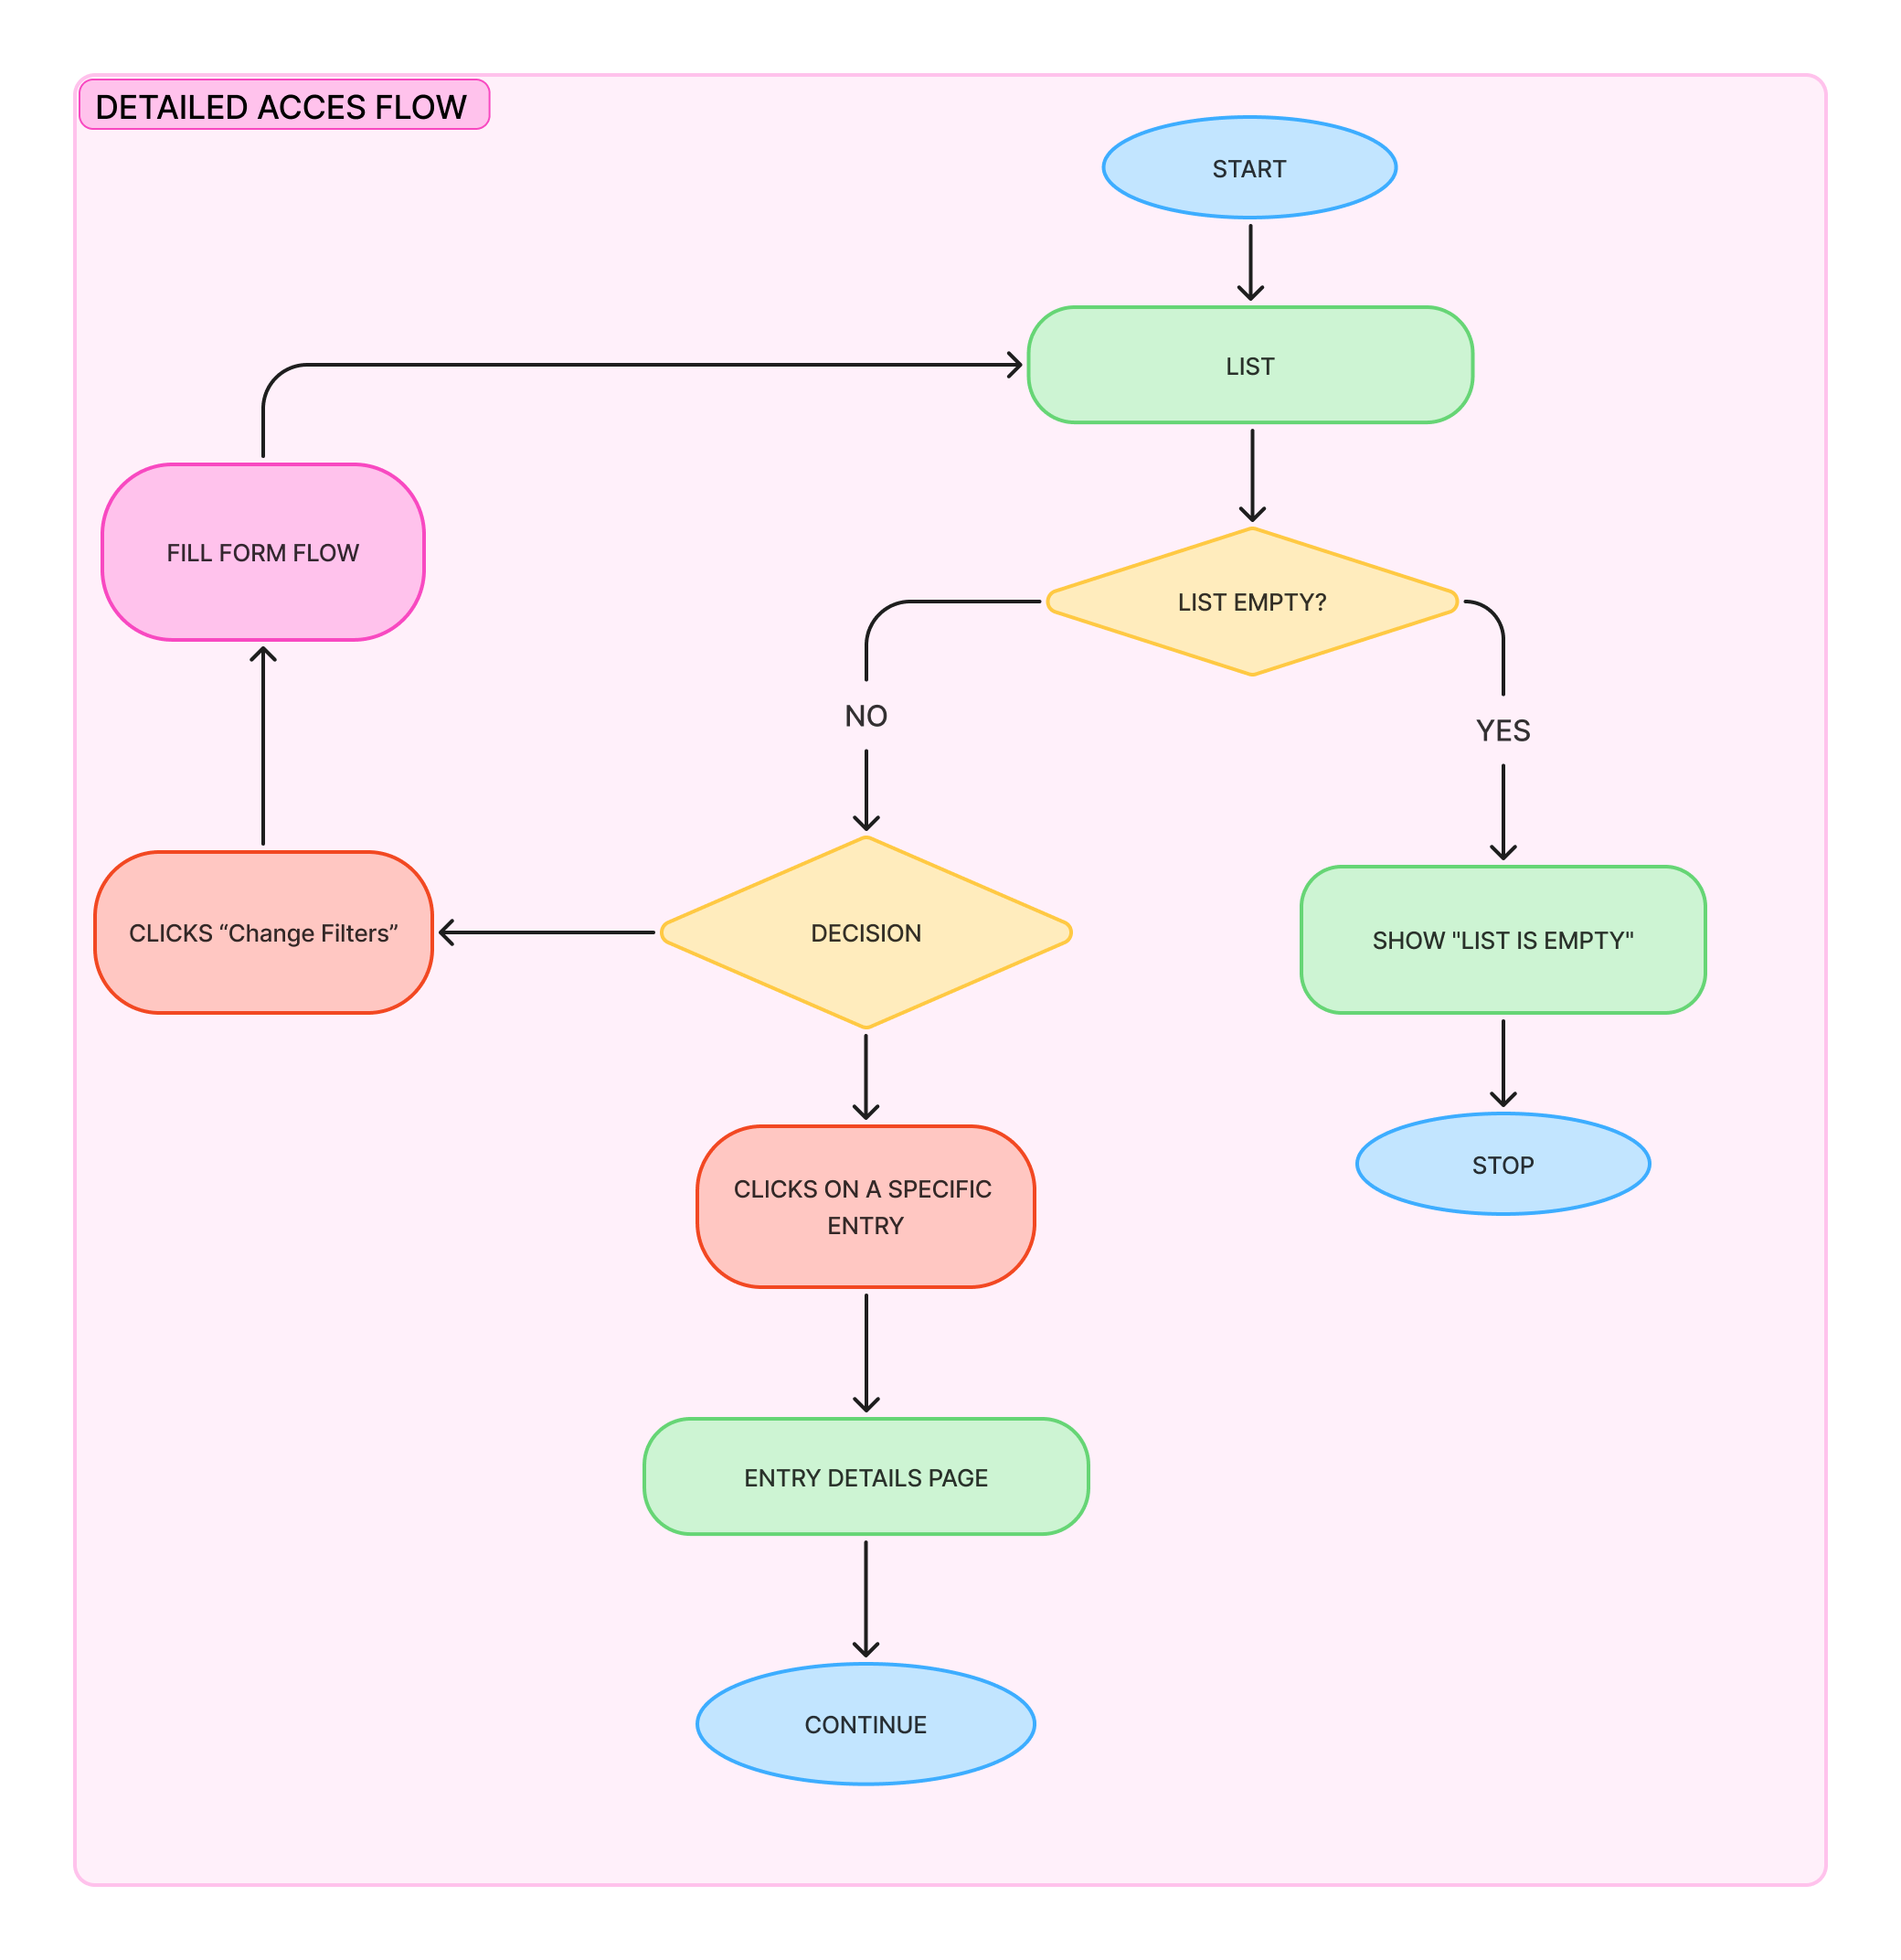
\includegraphics[width=9cm]{User_Flows/DetailedAccess.png}
        \captionof{figure}{General Detailed Access Flow}
    \end{center}
    %\begin{itemize}   
    %\end{itemize}
\end{minipage}
\vspace{3em}

\begin{minipage}{\textwidth}
    \phantomsection 
    \subsection{General Flow - Creation Flow}
    The following diagram describes in detail the steps of the general Creation flow, expanded in the user flow \hyperref[UF6]{UF6. Admin - Create Insurance Policy, Hospital, Treatment, Department. Register Doctor}.
    
    \begin{center}
        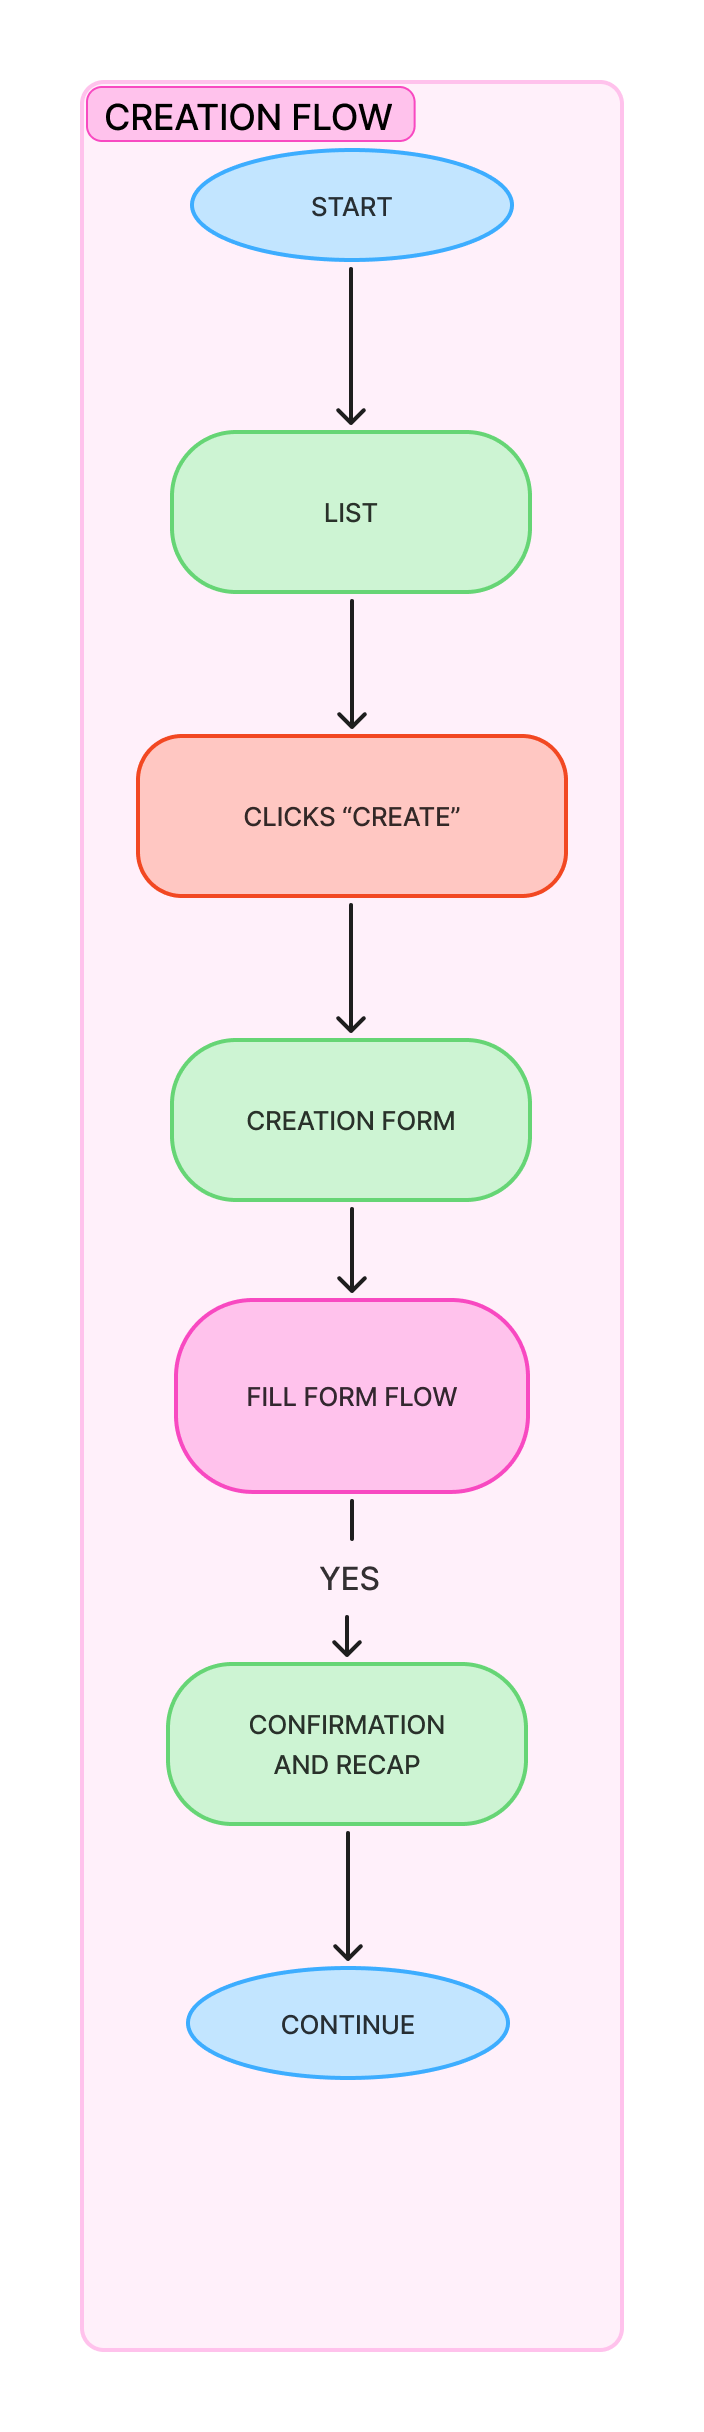
\includegraphics[width=5cm]{User_Flows/Creation.png}
        \captionof{figure}{General Creation Flow}
    \end{center}
    %\begin{itemize}   
    %\end{itemize}
\end{minipage}
\vspace{3em}

\begin{minipage}{\textwidth}
    \phantomsection
    \subsection{General Flow - Edit Flow}
    The following diagram describes in detail the steps of the general Edit flow, expanded in the user flow \hyperref[UF7]{UF7. Admin - Edit Insurance Policy, Hospital, Treatment, Department. Register Doctor}.
    \begin{center}
        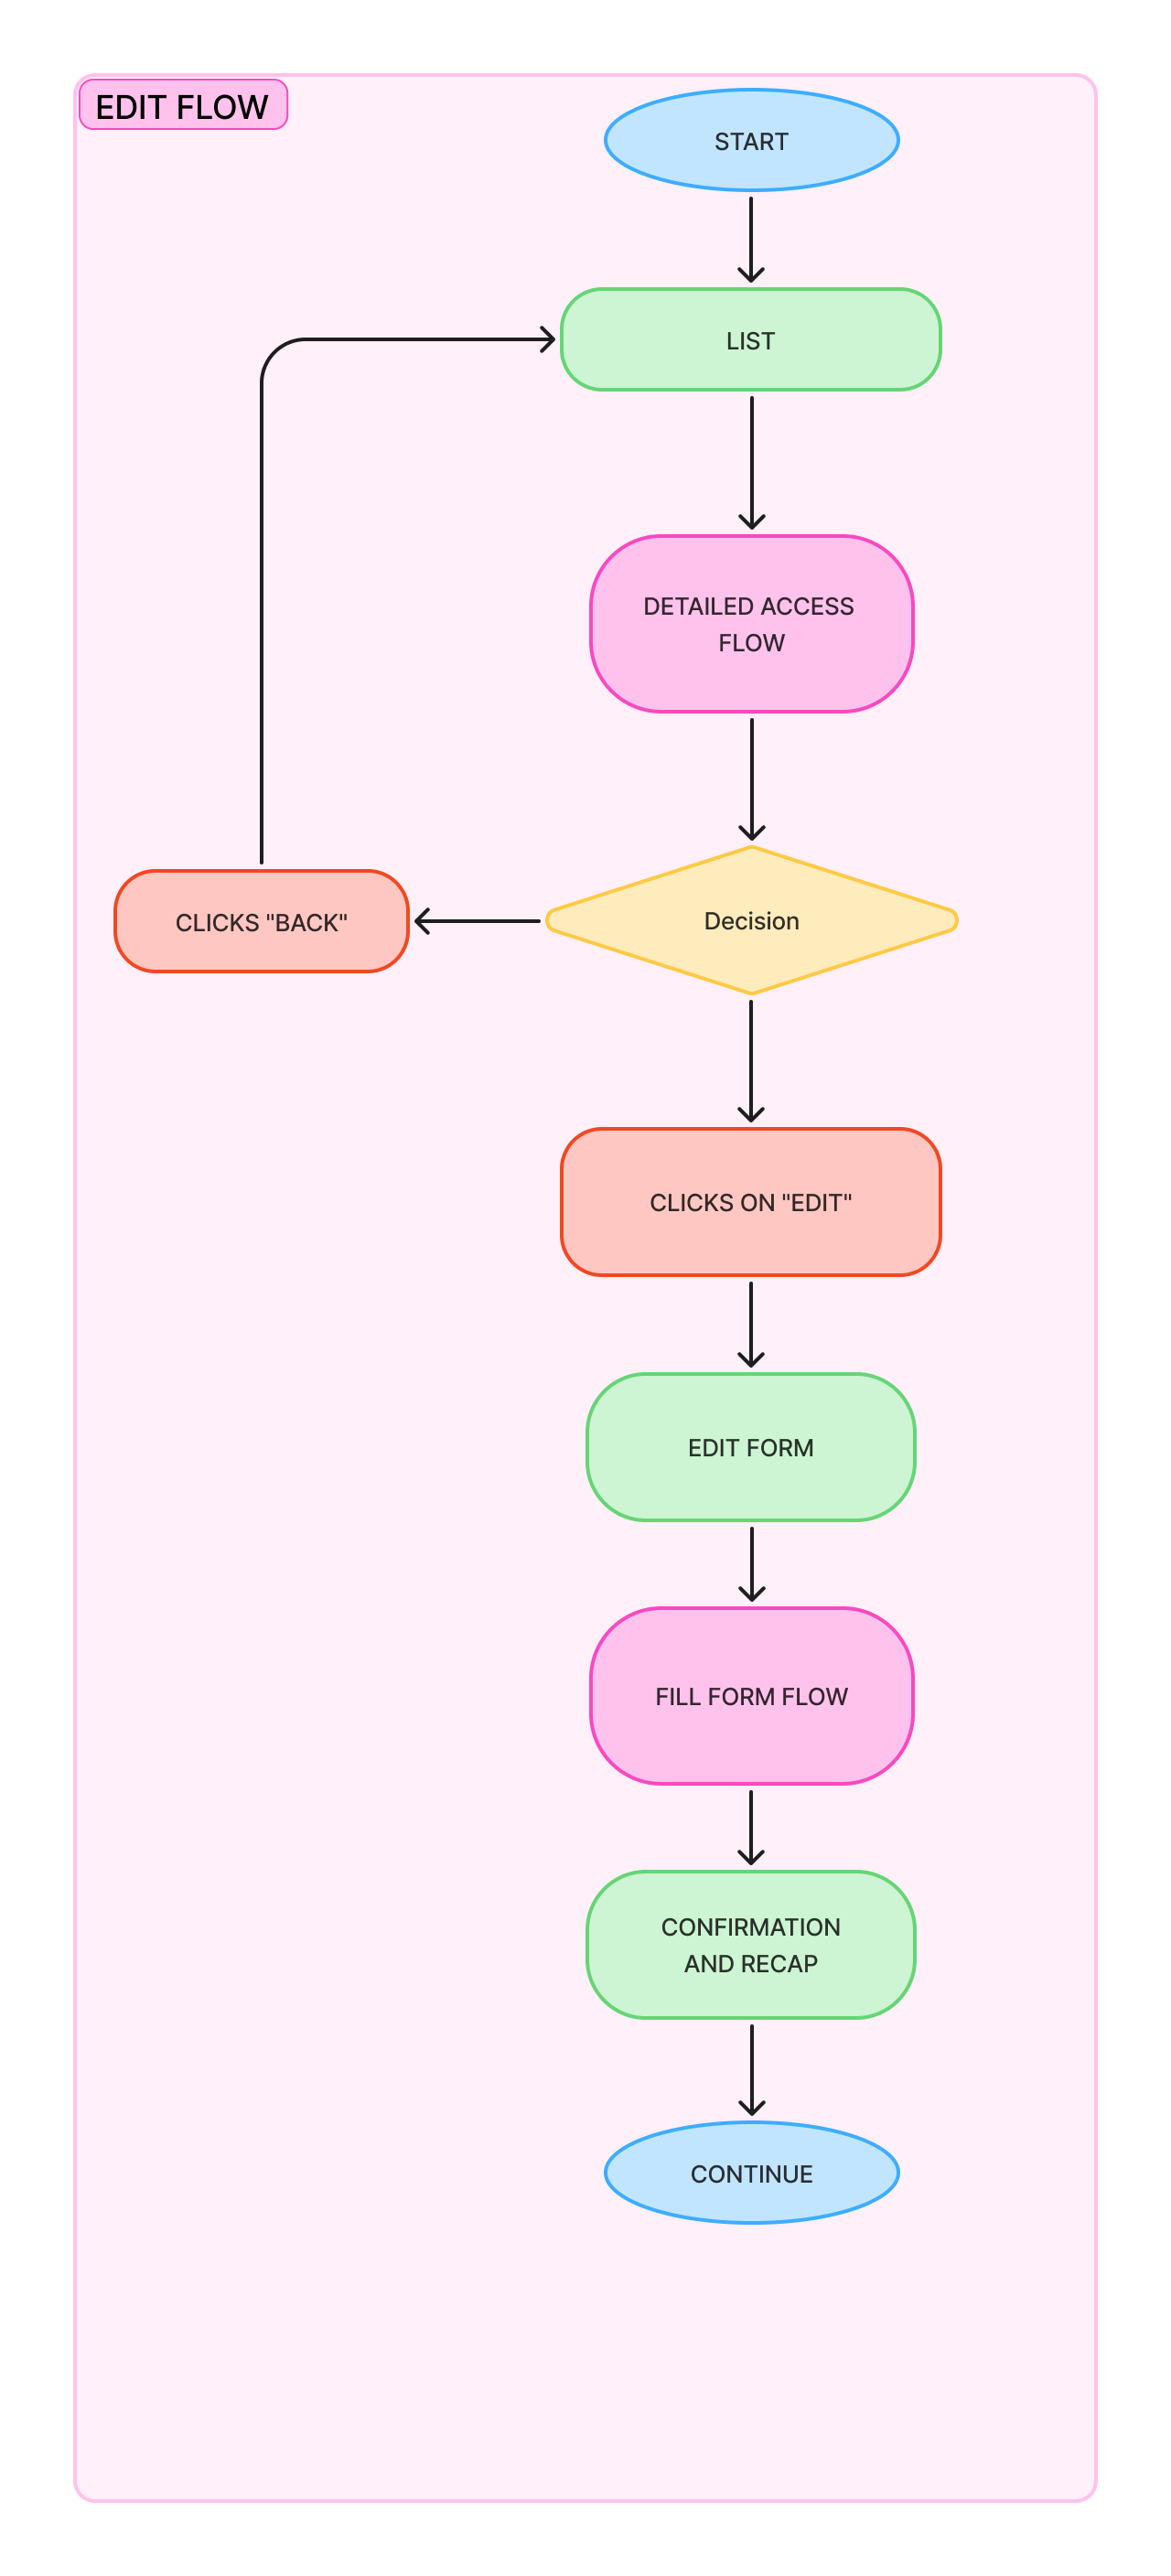
\includegraphics[width=8cm]{User_Flows/Edit.png}
        \captionof{figure}{General Edit Flow}
    \end{center}
    %\begin{itemize}   
    %\end{itemize}
\end{minipage}
\vspace{3em}

\begin{minipage}{\textwidth}
    \phantomsection
    \subsection{General Flow - Deletion Flow}
    The following diagram describes in detail the steps of the general Deletion flow, expanded in the user flow \hyperref[UF8]{UF8. Admin - Deactivate Insurance Policy, Hospital, Treatment, Department}.
    
    \begin{center}
        
\includegraphics[width=8cm]{User_Flows/Deletion.png}
        \captionof{figure}{General Deletion Flow}
    \end{center}
    %\begin{itemize}   
    %\end{itemize}
\end{minipage}
\vspace{3em}

\begin{minipage}{\textwidth}
    \phantomsection
    \subsection{UF1. User - Login and Recovery}
    The following user flow shows the process of User login and account recovery. UC24 is implemented with mock IDP login, while UC26 is not implemented.
    It refers to use cases \textbf{UC24, UC26}, and methods \textbf{login(credentials), requestPasswordReset()} from the class \textbf{User} of the class diagram.
    
    \begin{center}
        
\includegraphics[width=0.8\textwidth]{User_Flows/LoginRecovery.png}
        \captionof{figure}{User flow regarding User Login and Recovery}
    \end{center}
    %\begin{itemize}   
    %\end{itemize}
\end{minipage}
\vspace{3em}


\begin{minipage}{\textwidth}
    \phantomsection
    \subsection{UF2. User - Internal Calendar}
    The following user flow shows the steps a user takes to view their calendar and see the details of a booked appointment. UC28, UC38 are implemented.
    It refers to use cases \textbf{UC30, UC28}, and methods \textbf{Calendar.getAppointments(), Appointment.getDetails()} from the class \textbf{Calendar, Appointment} of the class diagram.
    
    \begin{center}
        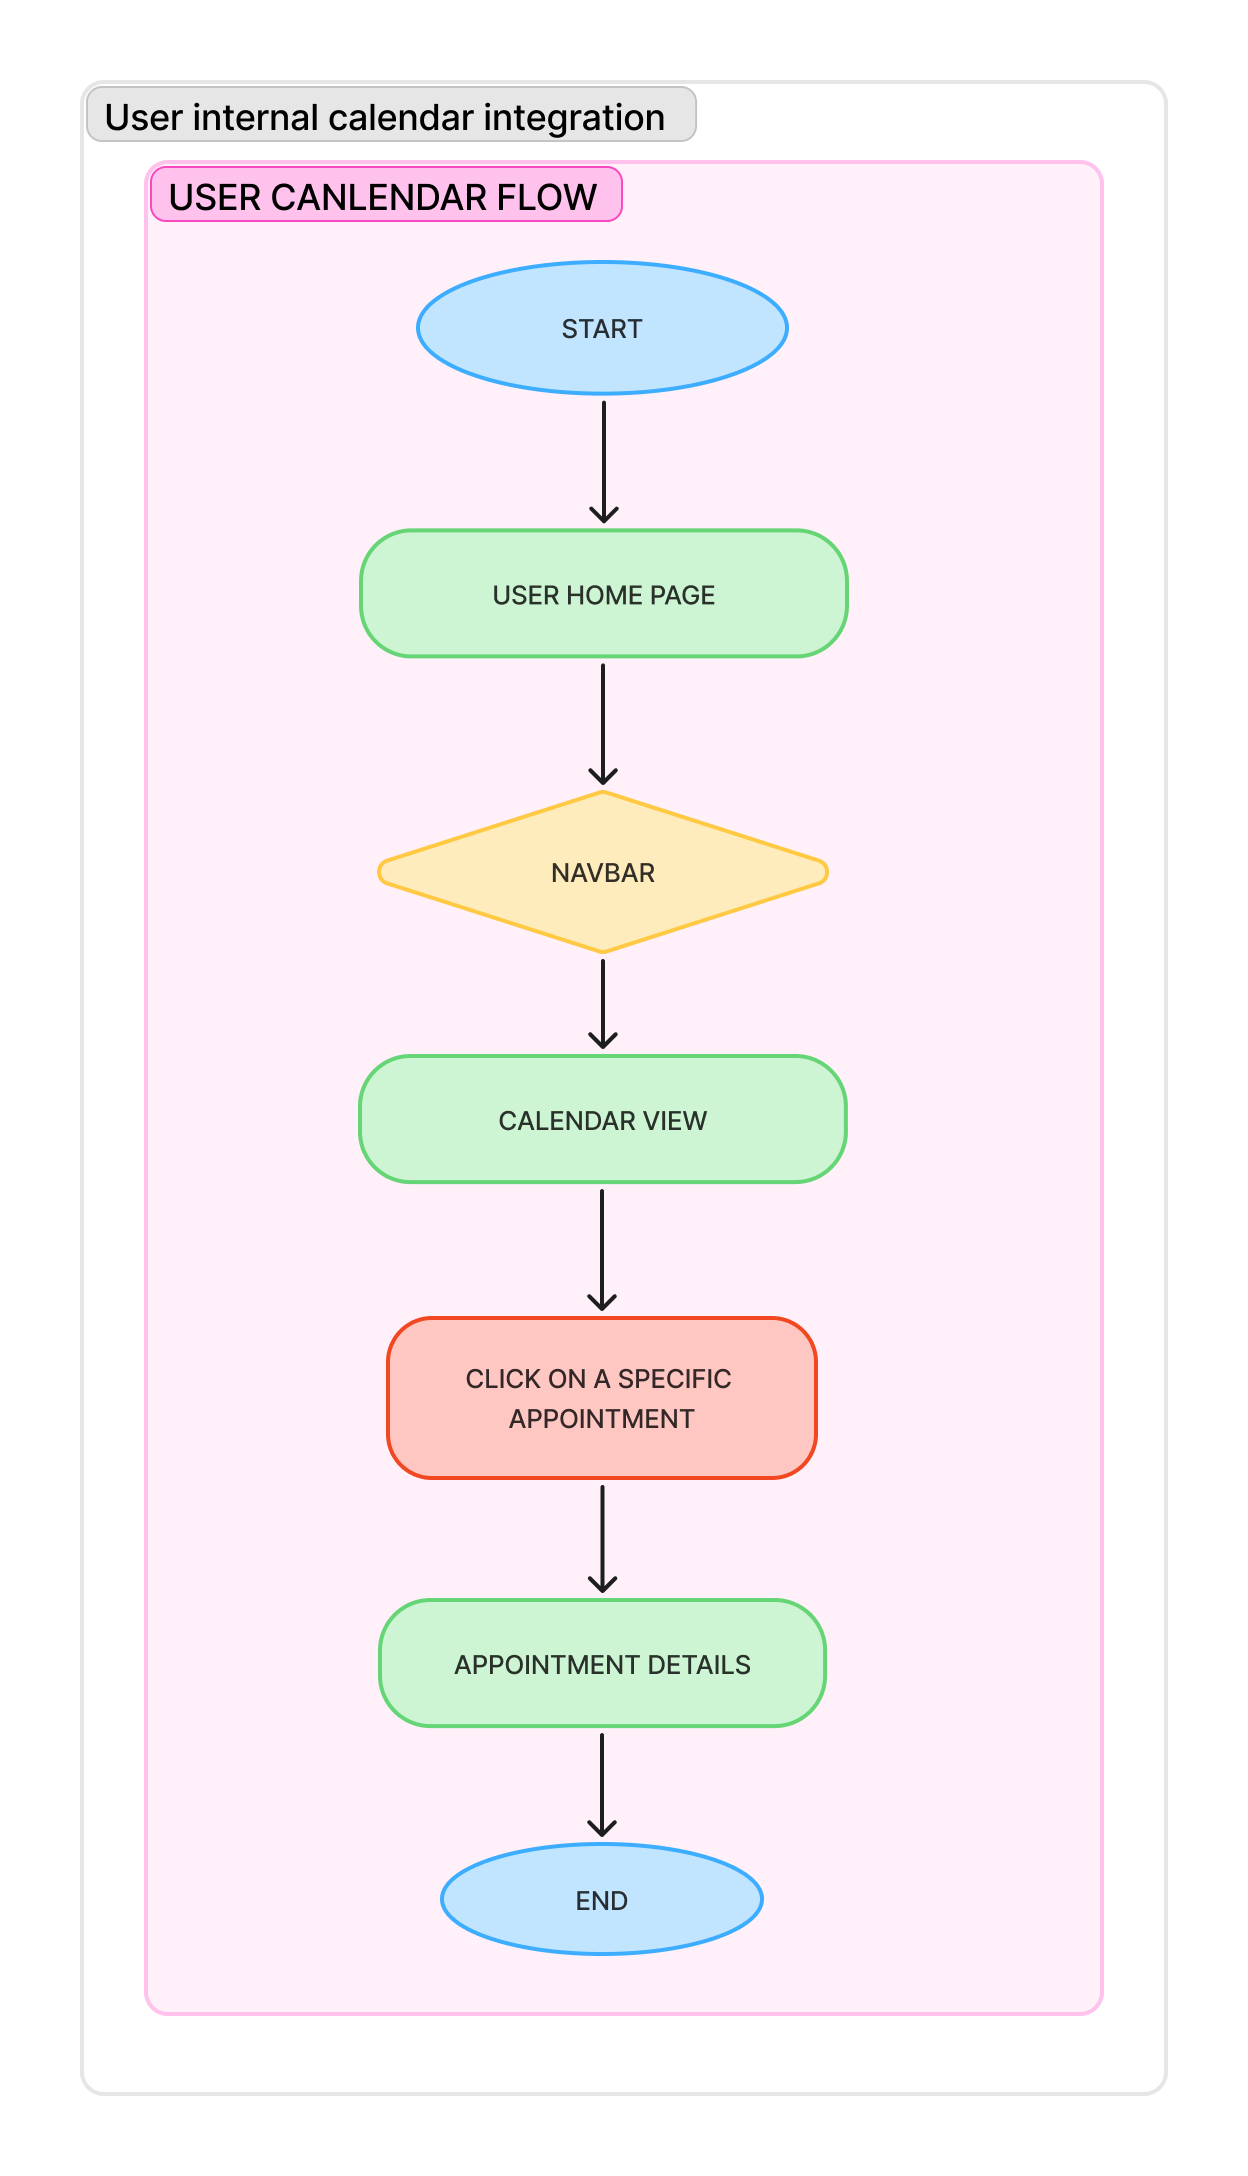
\includegraphics[width=8cm]{User_Flows/UserInternalCalendar.png}
        \captionof{figure}{User flow regarding Internal Calendar integration and View Appointment Details}
    \end{center}
    %\begin{itemize}   
    %\end{itemize}
\end{minipage}
\vspace{3em}


\begin{minipage}{\textwidth}
    \phantomsection
    \subsection{UF3. User - Profile Update and Deletion}
    The following user flow shows the steps a user takes to update and delete their profile. UC7 is implemented, UC41 is partially implemented as the deletion of the account occurs immediately rather than after 30 days.
    It refers to use cases \textbf{UC7, UC41}, and methods \textbf{viewProfile(), updateProfile(newData), deleteAccount()} from the class \textbf{User} of the class diagram.
    
    \begin{center}
        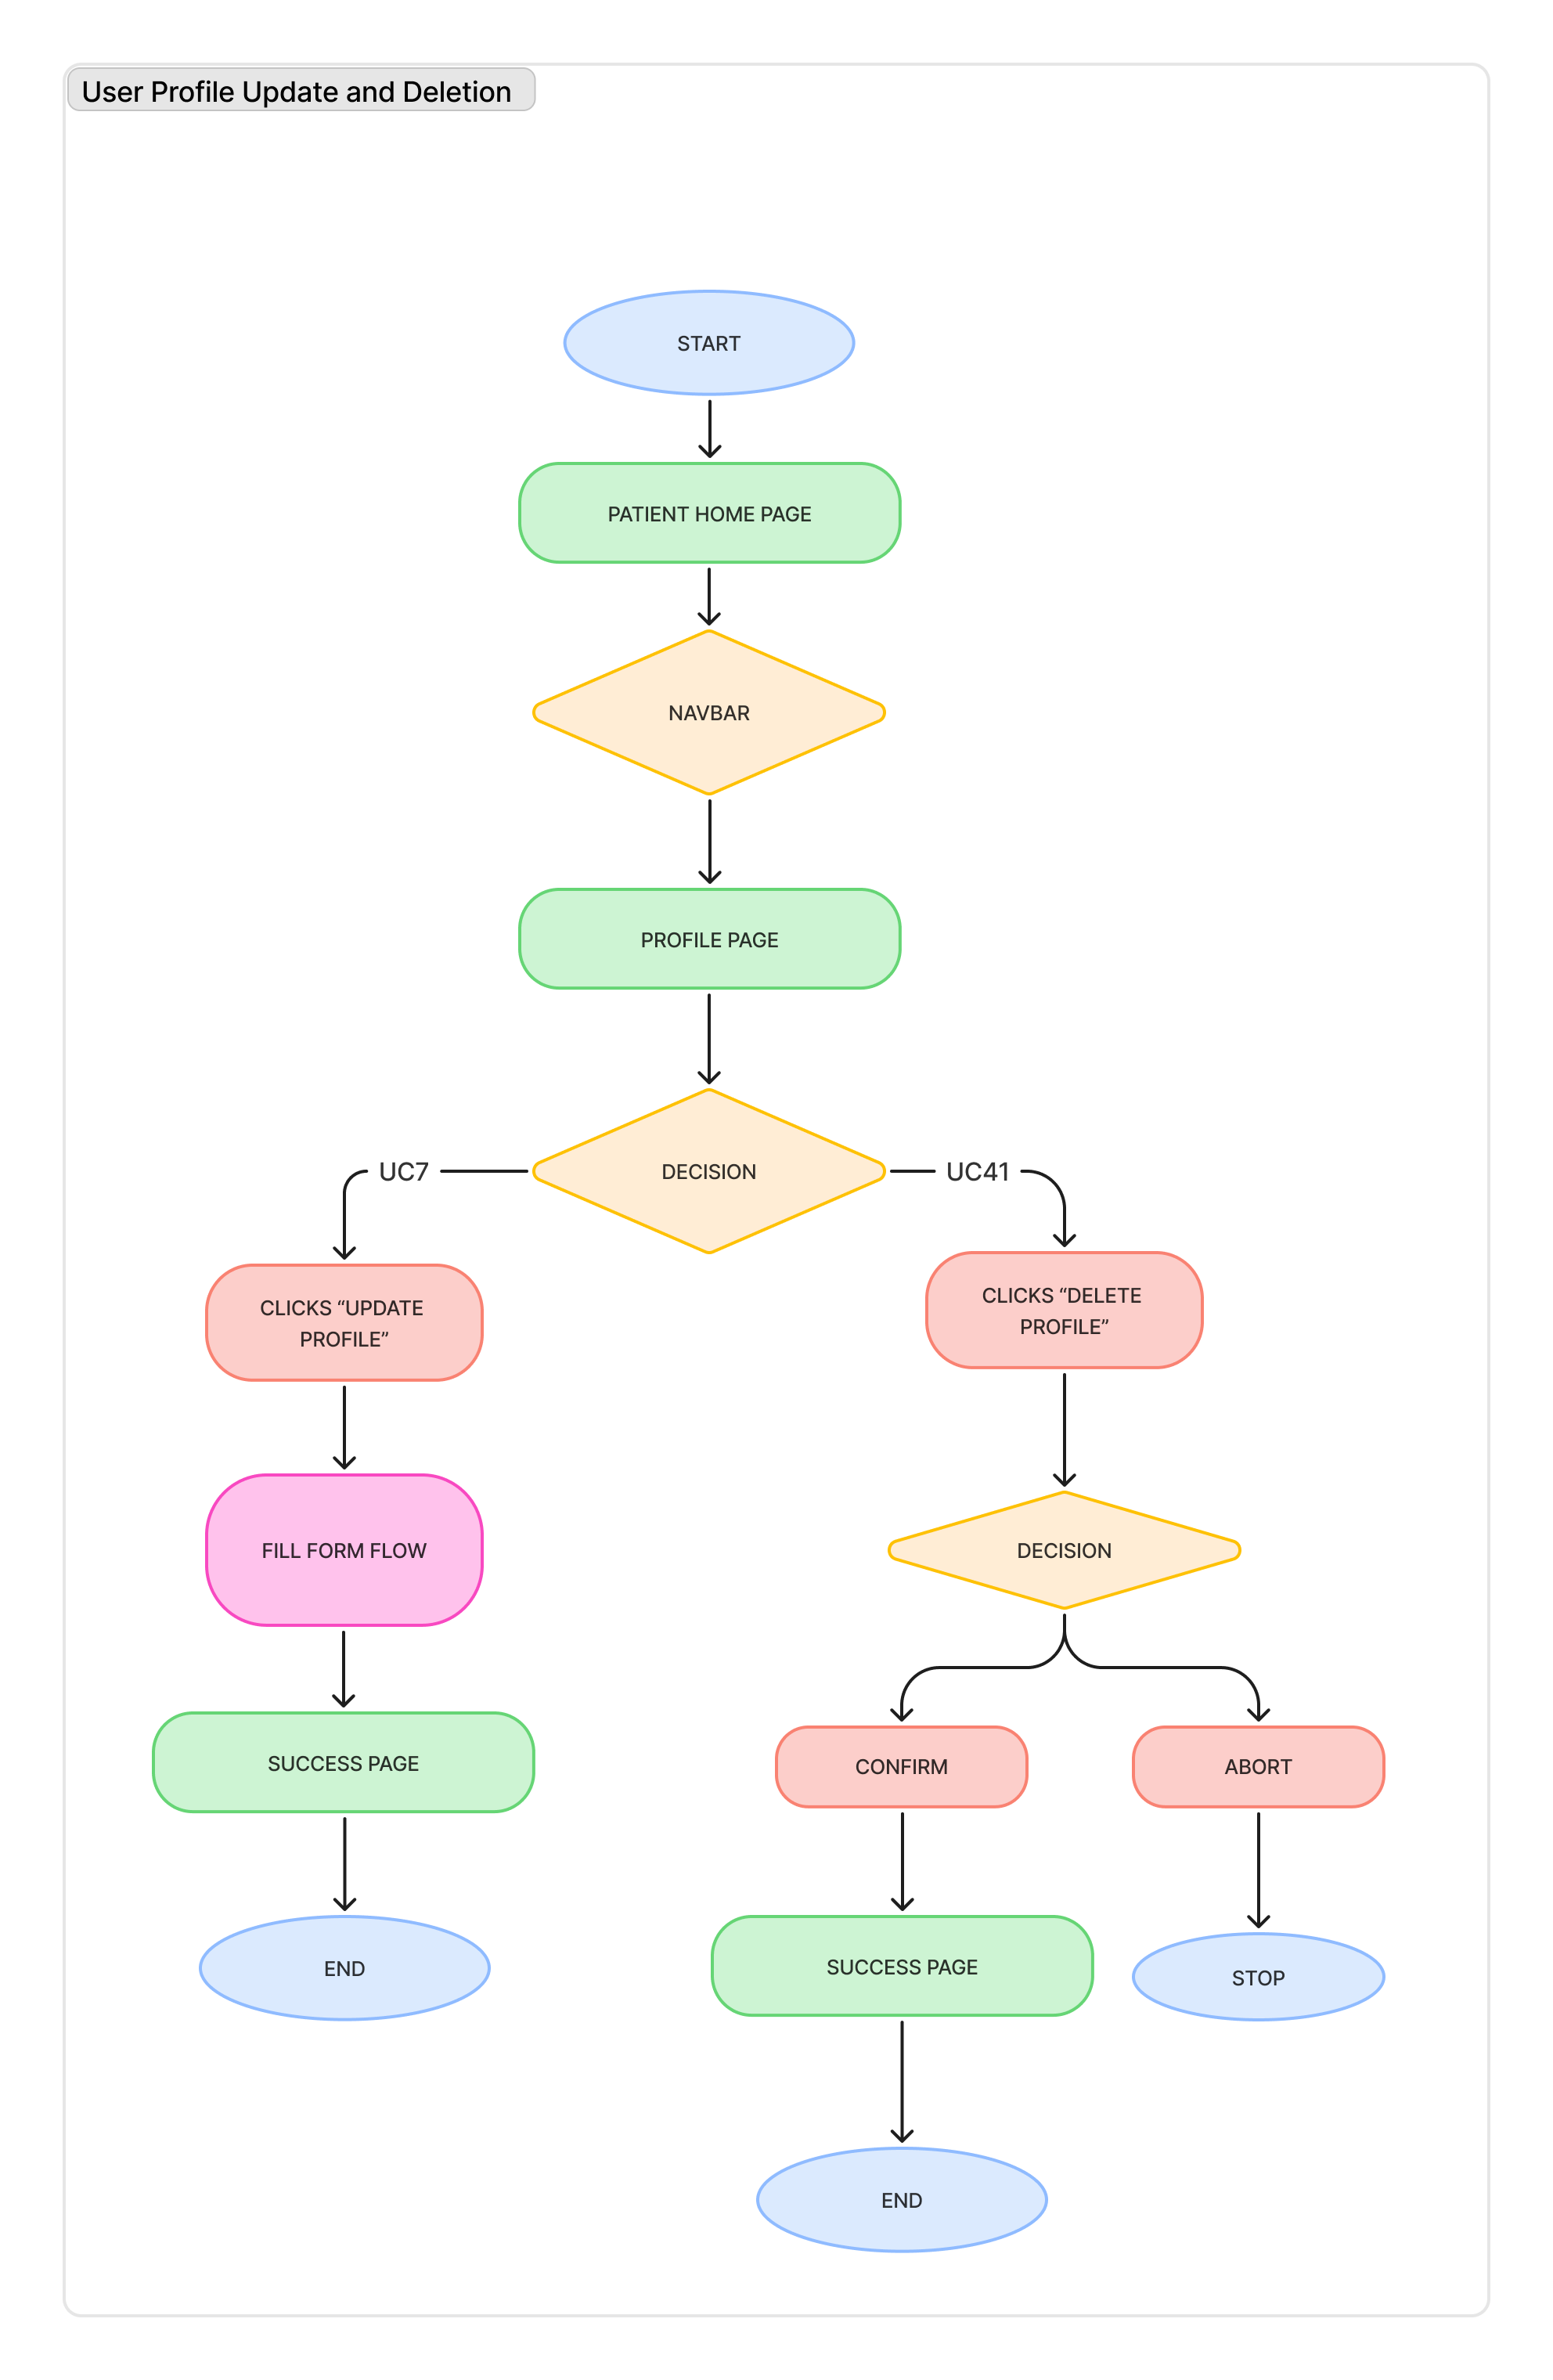
\includegraphics[width=0.8\textwidth]{User_Flows/ProfileUpdateDeletion.png}
        \captionof{figure}{User flow regarding Profile Update and Account Deletion}
    \end{center}
    %\begin{itemize}   
    %\end{itemize}
\end{minipage}
\vspace{3em}

\begin{minipage}{\textwidth}
    \phantomsection
    \subsection{UF4. User - Export Calendar}
    The following user flow shows the steps a user takes to export their appointment to an external calendar. UC31 is not implemented.
    It refers to use case \textbf{UC31}, and methods \textbf{generateExportToken()} from the class \textbf{Calendar} of the class diagram.
    
    \begin{center}
        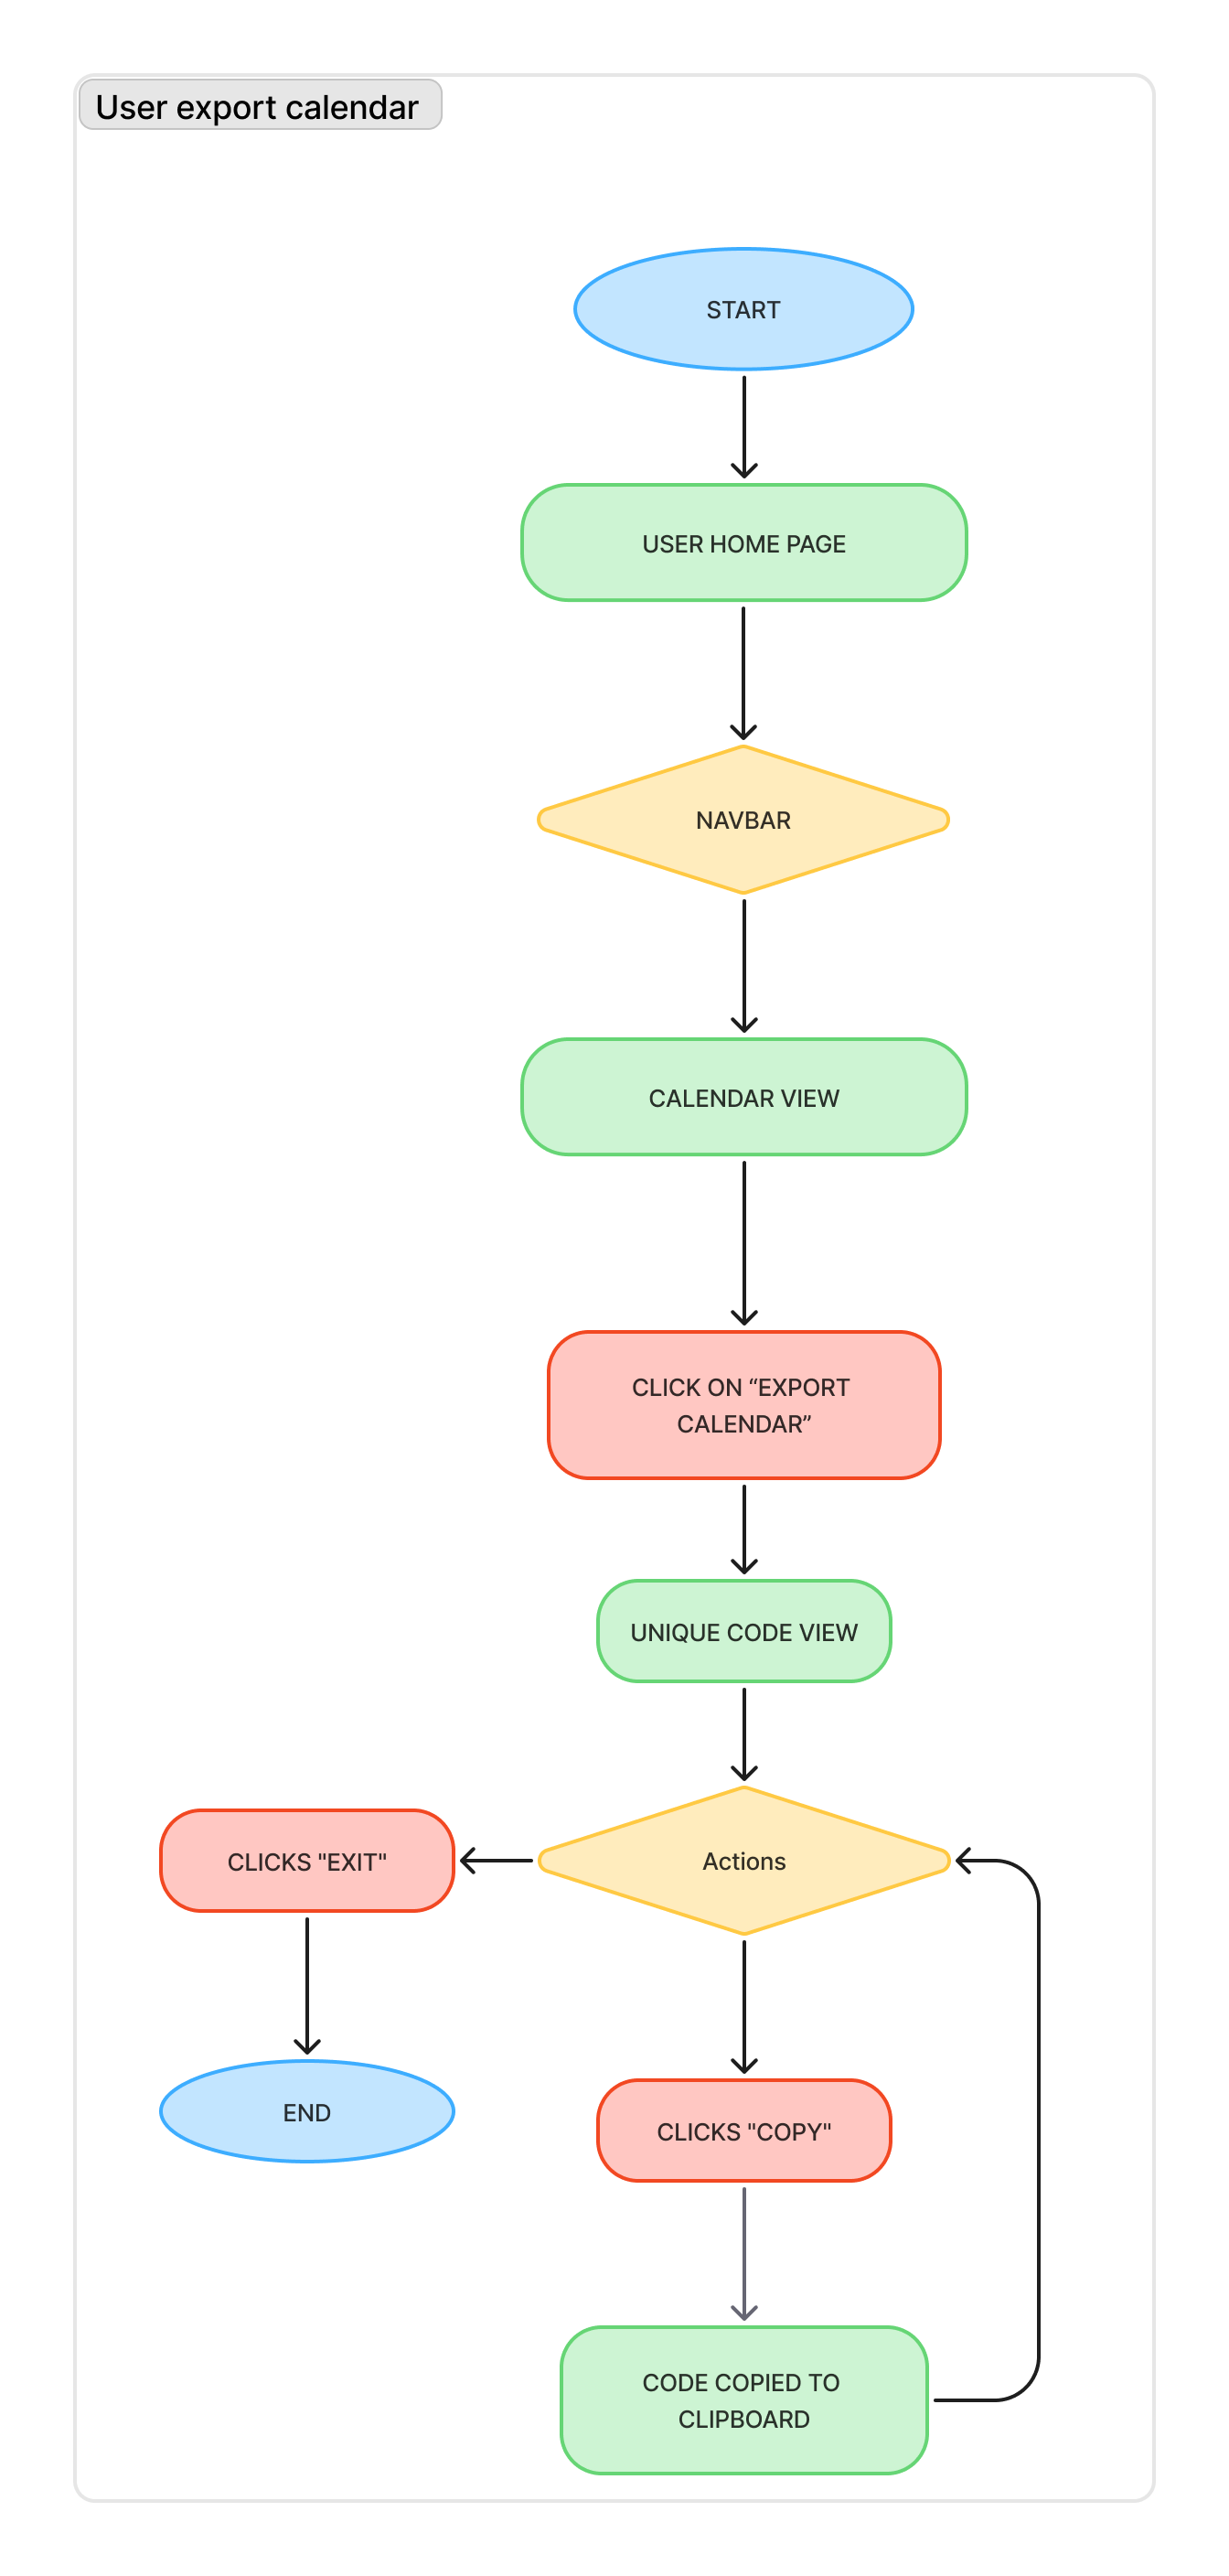
\includegraphics[width=8cm]{User_Flows/ExportCalendar.png}
        \captionof{figure}{User flow regarding Appointment export}
    \end{center}
    %\begin{itemize}   
    %\end{itemize}
\end{minipage}
\vspace{3em}

\begin{minipage}{\textwidth}
    \phantomsection
    \subsection{UF5. Admin - Login}
    The following user flow shows the steps the admin takes to login. UC45 is implemented.
    It refers to use case \textbf{UC45}, and method \textbf{adminLogin(credentials)} from the class \textbf{SystemAdmin} of the class diagram.
    
    \begin{center}
        
\includegraphics[width=8cm]{User_Flows/AdminLogin.png}
        \captionof{figure}{User flow regarding Admin Login}
    \end{center}
    %\begin{itemize}   
    %\end{itemize}
\end{minipage}
\vspace{3em}

\begin{minipage}{\textwidth}
    \phantomsection
    \subsection{UF6. Admin - Create Insurance Policy, Hospital, Treatment, Department. Register Doctor}
    \label{UF6}
    The following user flow shows the steps the admin takes to create an Insurance Policy, Hospital, Treatment, Department and register a Doctor. UC1, UC2, UC12 are implemented.
    It refers to use cases \textbf{UC1, UC2, UC12}, and methods \textbf{InsurancePolicy.create(policyData), Hospital.create(hospitalData), Treatment.create(treatmentData), SystemAdmin.createDepartment(hospital, departmentData), SystemAdmin.registerDoctor(doctorData)} from the classes \textbf{InsurancePolicy, Hospital, Treatment, SystemAdmin} of the class diagram.
    
    \begin{center}
        
\includegraphics[width=0.8\textwidth]{User_Flows/CreatePolicyHospitalTreatmentDepartment.png}
        \captionof{figure}{User flow regarding Admin Create Insurance Policy, Hospital, Treatment, Department. Register Doctor}
    \end{center}
    %\begin{itemize}   
    %\end{itemize}
\end{minipage}
\vspace{3em}

\begin{minipage}{\textwidth}
    \phantomsection
    \subsection{UF7. Admin - Edit Insurance Policy, Hospital, Treatment, Department}
    \label{UF7}
    The following user flow shows the steps the admin takes to edit an Insurance Policy, Hospital, Treatment, Department. UC5 and UC6 are implemented.
    It refers to use cases \textbf{UC5, UC6}, and methods \textbf{InsurancePolicy.edit(policy, newPolicyData), Hospital.edit(hospital, newHospitalData), Treatment.edit(treatment, newTreatmentData), Department.edit(department, newDepartmentData)} from the classes \textbf{InsurancePolicy, Hospital, Treatment, Department} of the class diagram.
    
    \begin{center}
        
\includegraphics[width=0.8\textwidth]{User_Flows/EditPolicyHospitalTreatmentDepartment.png}
        \captionof{figure}{User flow regarding Edit Insurance Policy, Hospital, Treatment, Department}
    \end{center}
    %\begin{itemize}   
    %\end{itemize}
\end{minipage}
\vspace{3em}

\begin{minipage}{\textwidth}
    \phantomsection
    \subsection{UF8. Admin - Deactivate Insurance Policy, Hospital, Treatment, Department}
    \label{UF8}
    The following user flow shows the steps the admin takes to deactivate an Insurance Policy, Hospital, Treatment, Department. UC8 and UC9 are implemented.
    It refers to use cases \textbf{UC8, UC9}, and methods \textbf{InsurancePolicy.deactivate(policy), Hospital.close(), Treatment.deactivate(), Department.close()} from the classes \textbf{InsurancePolicy, Hospital, Treatment, Department} of the class diagram.
    
    \begin{center}
        
\includegraphics[width=0.8\textwidth]{User_Flows/DeactivatePolicyHospitalTreatmentDepartment.png}
        \captionof{figure}{User flow regarding Deactivate Insurance Policy, Hospital, Treatment, Department}
    \end{center}
    %\begin{itemize}   
    %\end{itemize}
\end{minipage}
\vspace{3em}

\begin{minipage}{\textwidth}
    \phantomsection
    \subsection{UF9. Admin - Appoint Head of Hospital}
    The following user flow shows the steps the admin takes to appoint a Head of Hospital. UC14 is implemented.
    It refers to use case \textbf{UC14}, and methods \textbf{appointHeadOfHospital(doctor, hospital)} from the class \textbf{SystemAdmin} of the class diagram.
    
    \begin{center}
        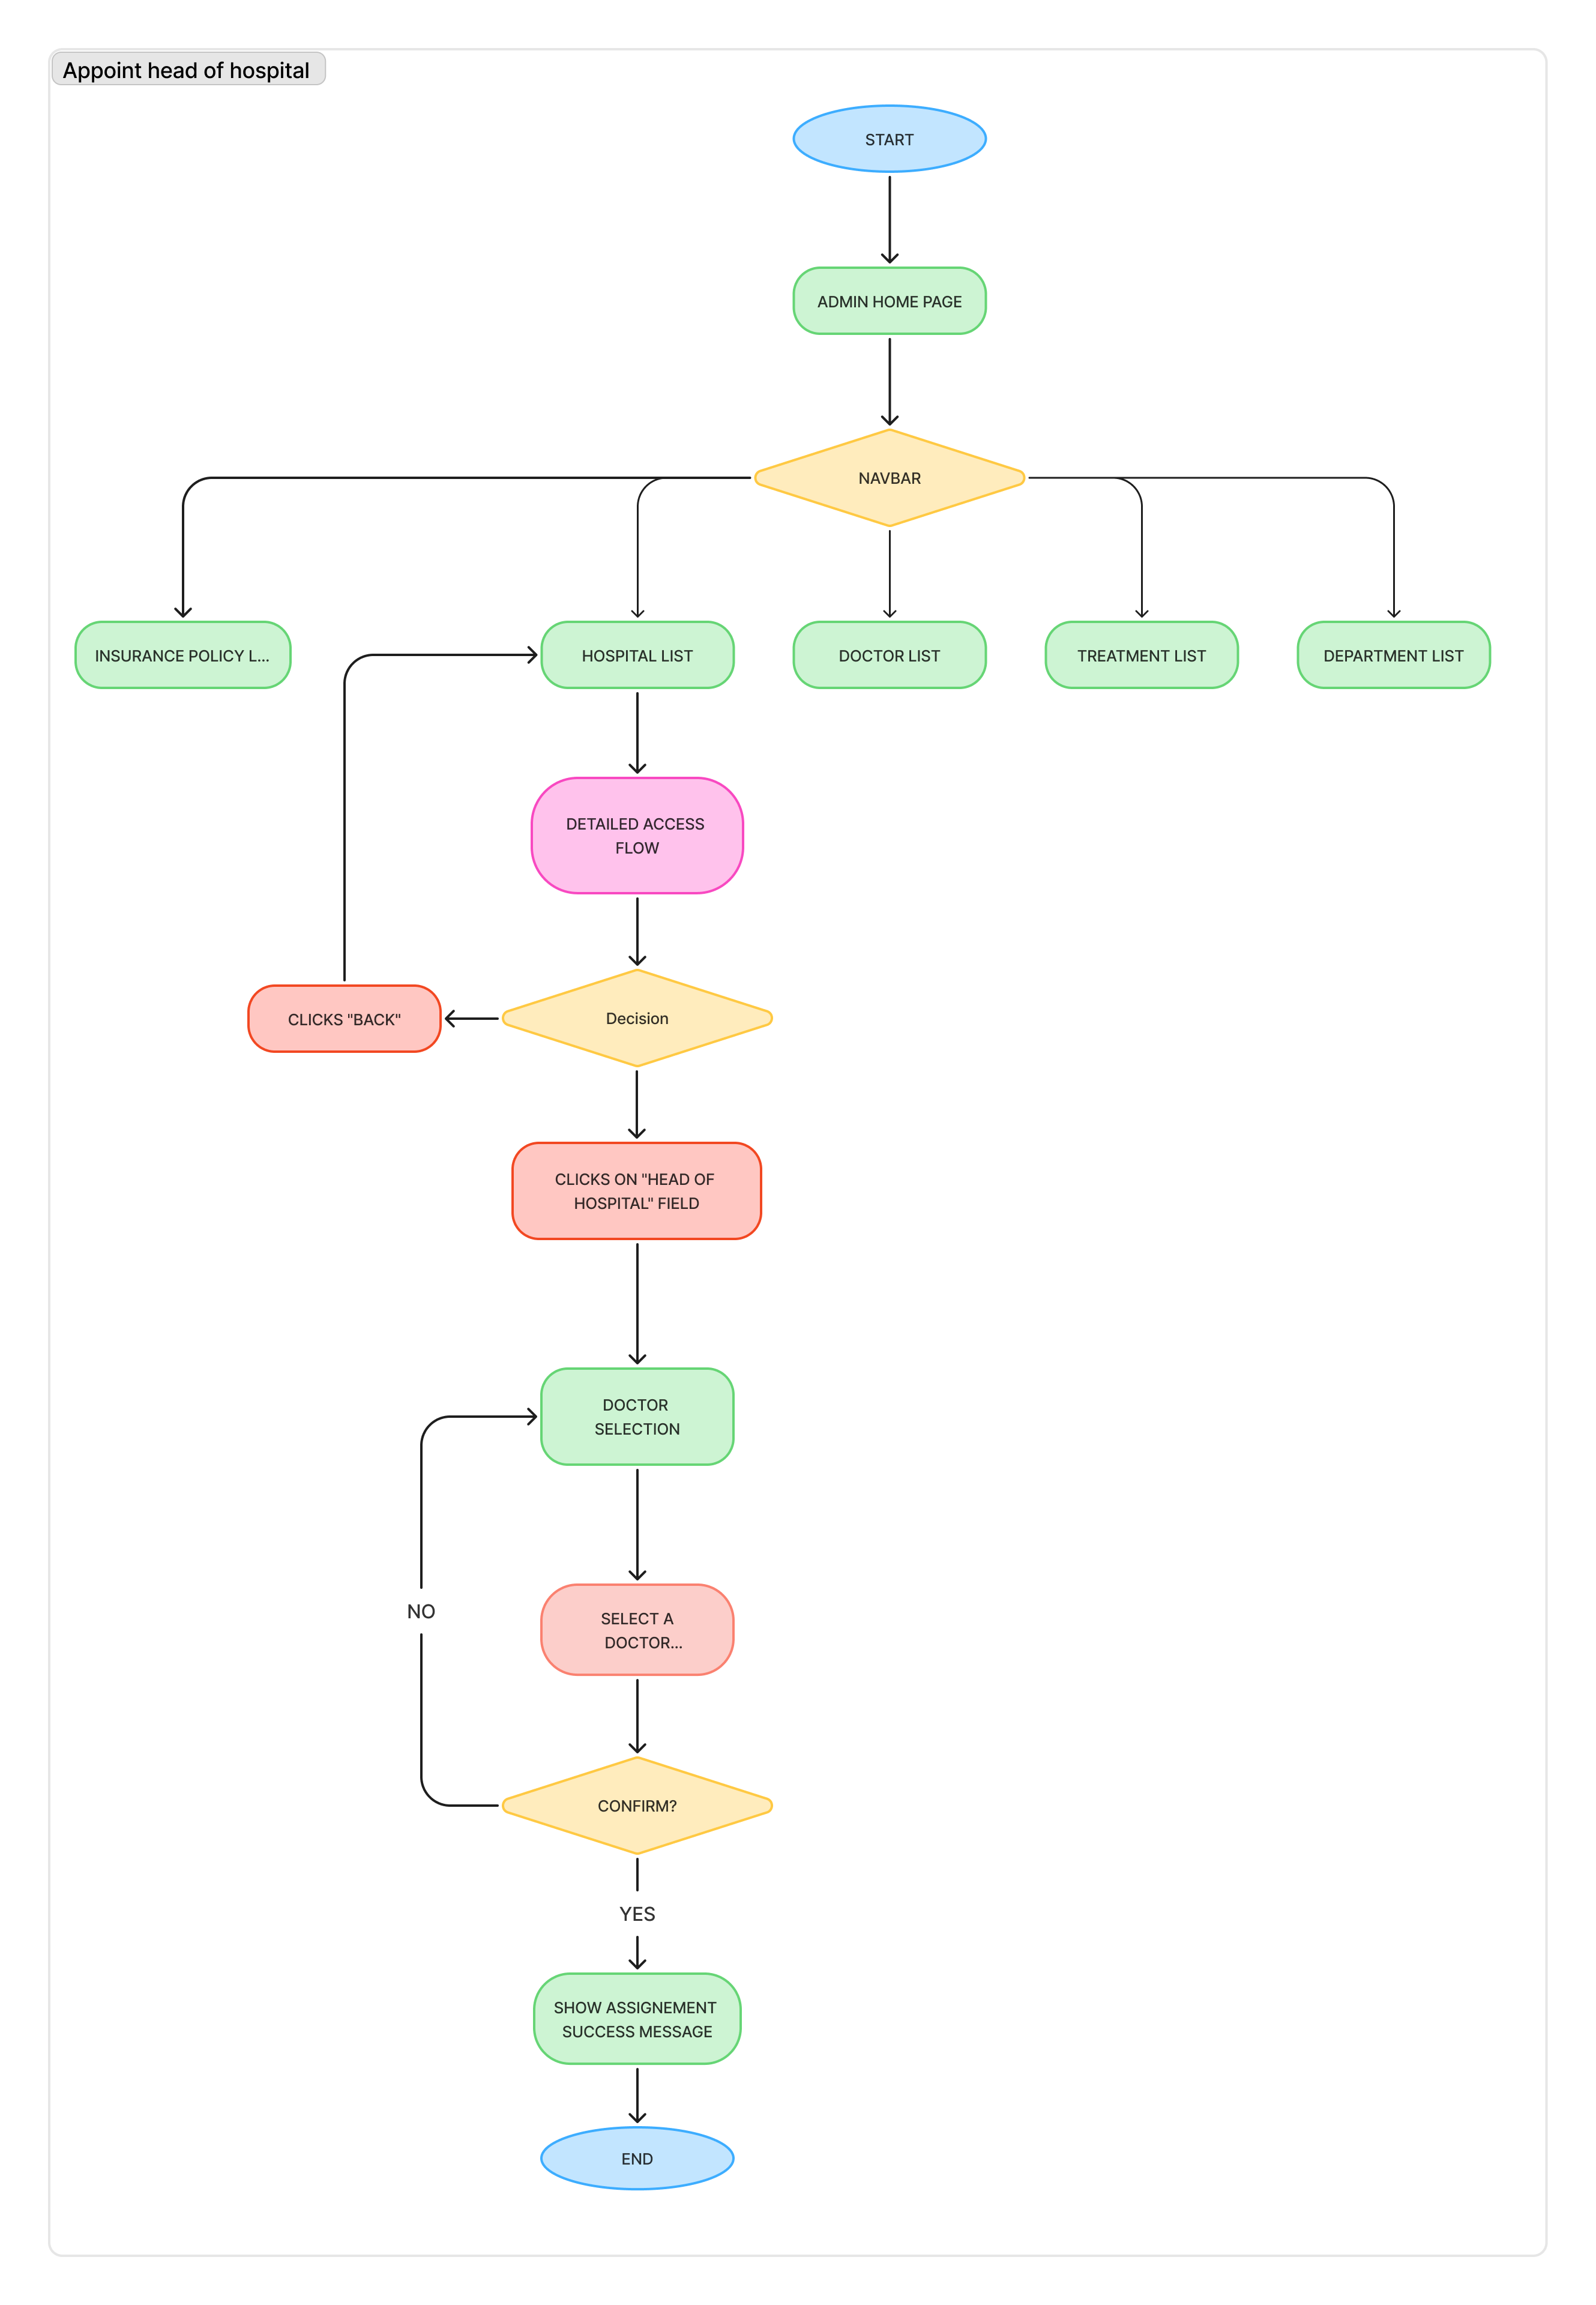
\includegraphics[width=0.8\textwidth]{User_Flows/AppointHeadOfHospital.png}
        \captionof{figure}{User flow regarding Appoint Head of Hospital}
    \end{center}
    %\begin{itemize}   
    %\end{itemize}
\end{minipage}
\vspace{3em}

\begin{minipage}{\textwidth}
    \phantomsection
    \subsection{UF10. Admin - Assign Doctor to Hospital}
    The following user flow shows the steps the admin takes to assign a doctor to a hospital. UC13 is implemented. 
    It refers to use case \textbf{UC13}, and methods \textbf{assignDoctorToHospital(doctor, hospital)} from the class \textbf{SystemAdmin} of the class diagram.
    
    \begin{center}
        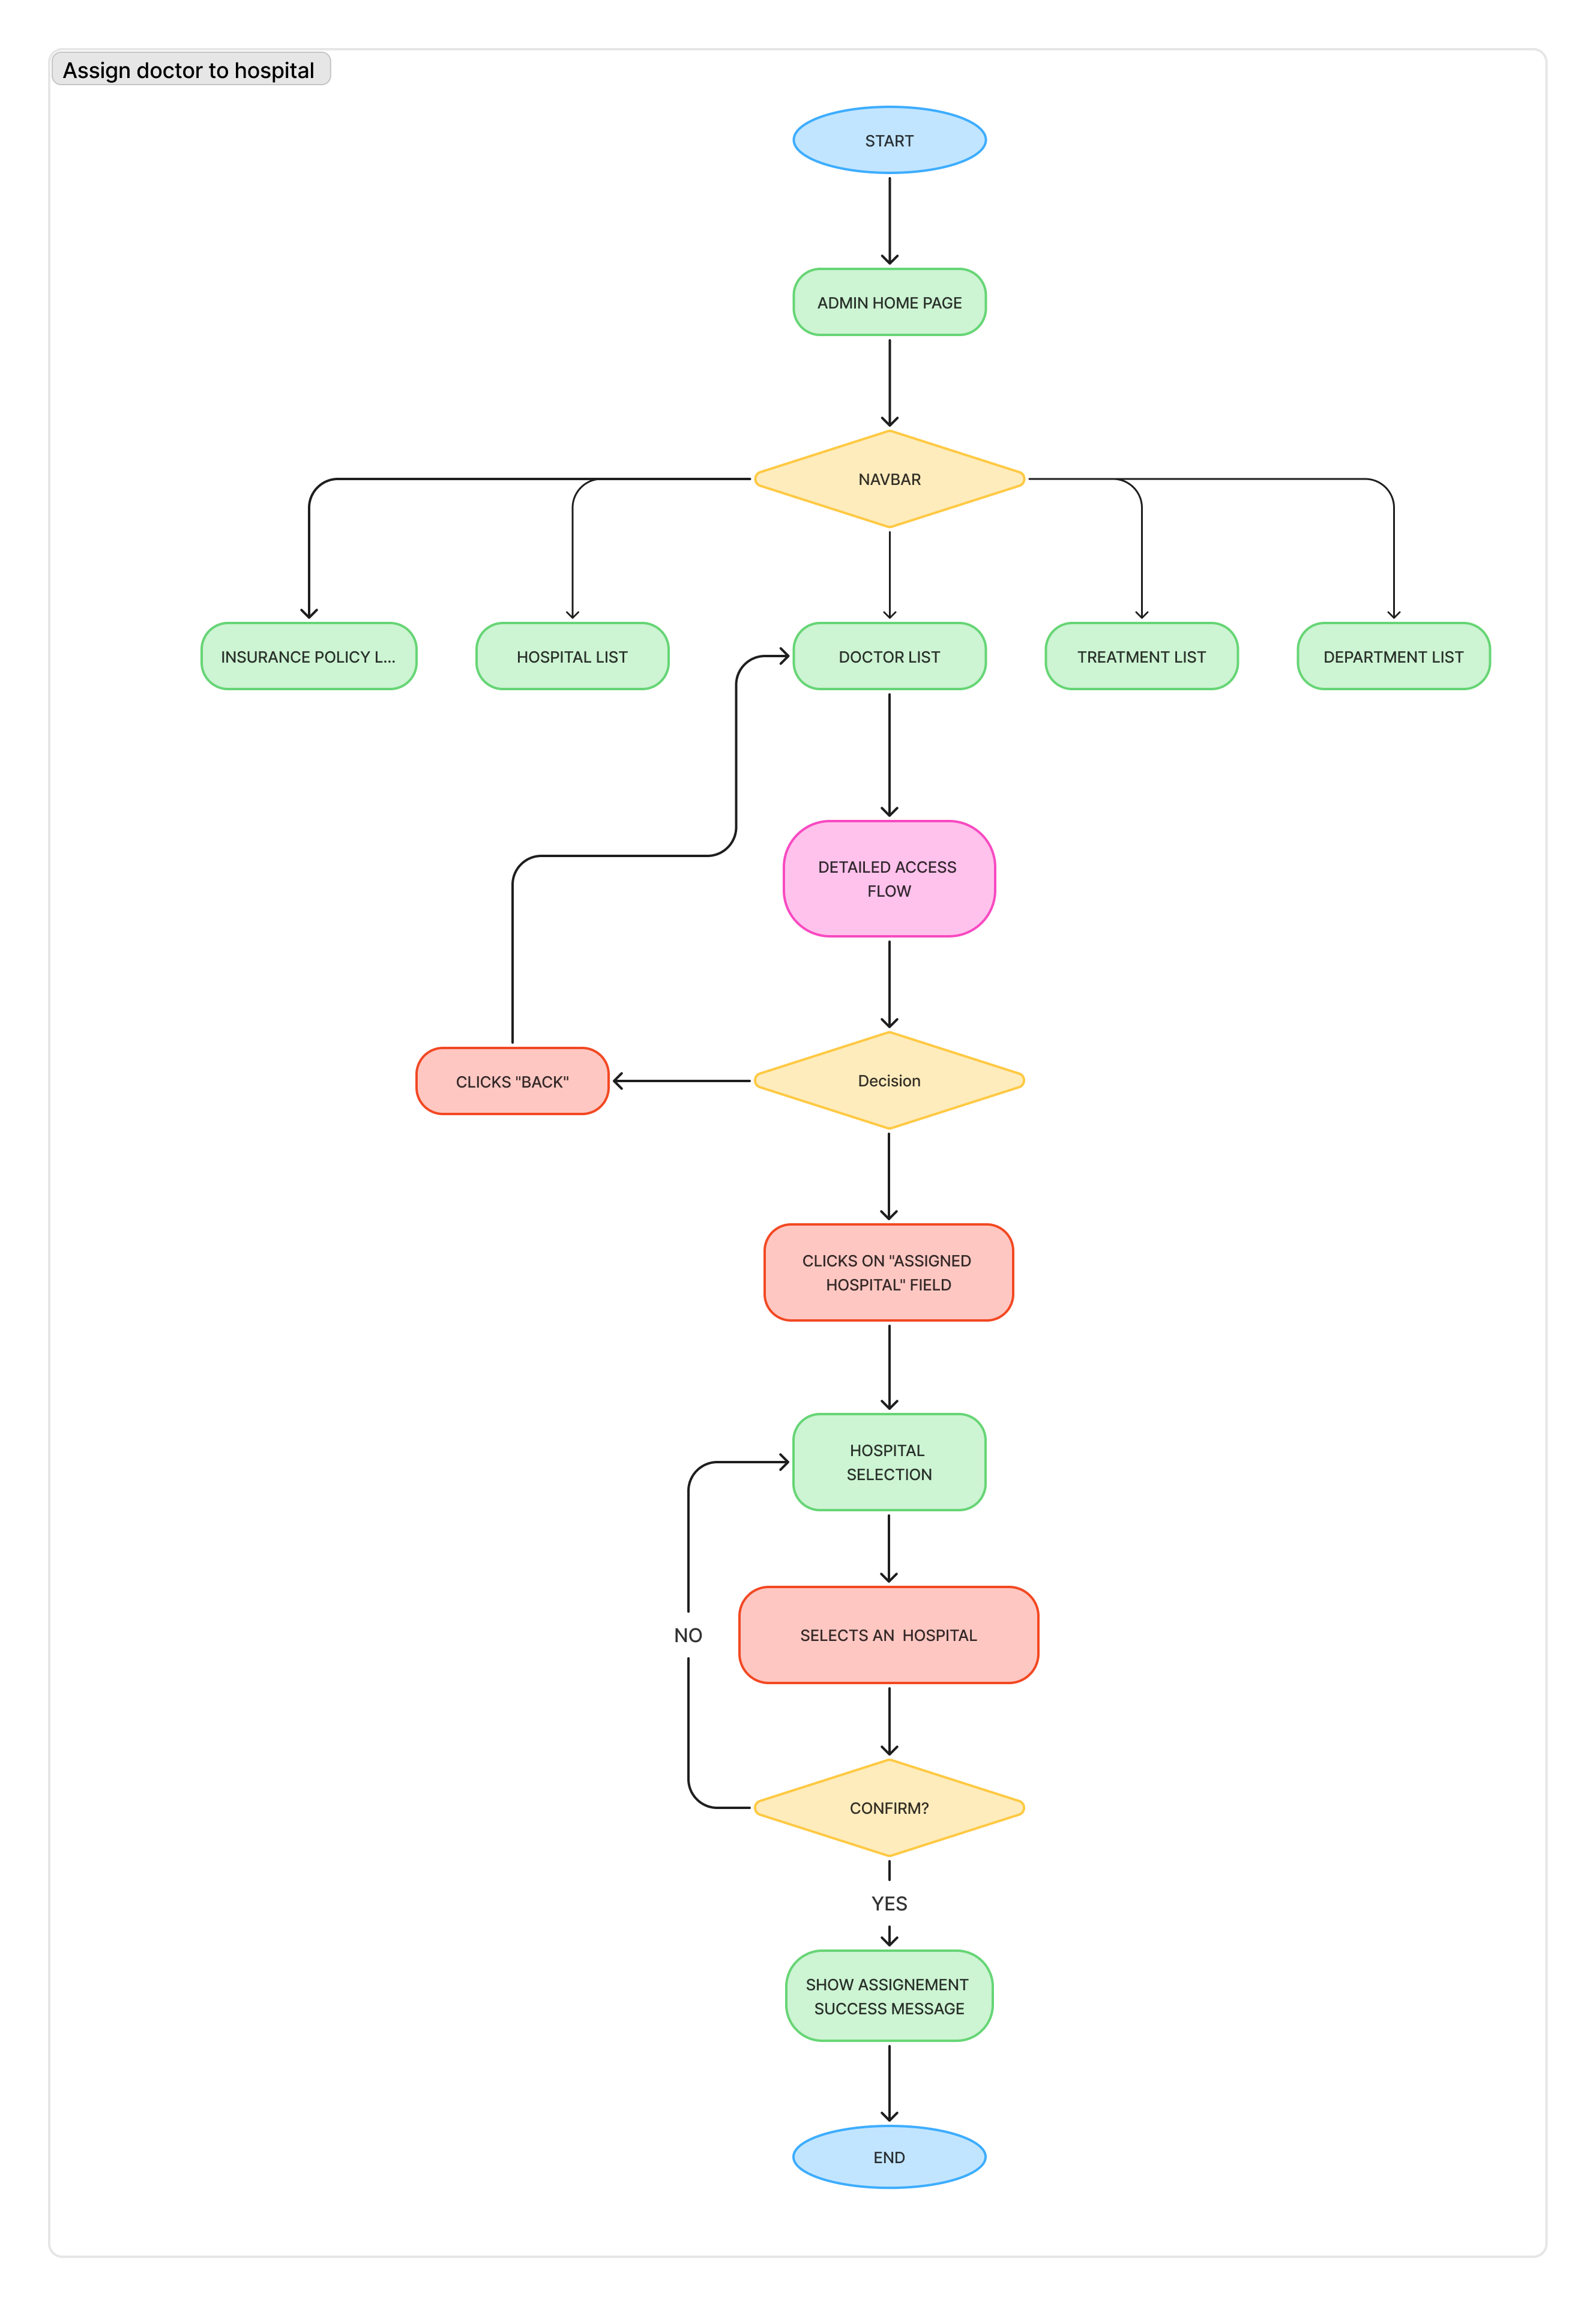
\includegraphics[width=0.8\textwidth]{User_Flows/AssignDoctorHospital.png}
        \captionof{figure}{User flow regarding Assign Doctor to Hospital}
    \end{center}
    %\begin{itemize}   
    %\end{itemize}
\end{minipage}
\vspace{3em}

\begin{minipage}{\textwidth}
    \phantomsection
    \subsection{UF11. Admin - Generate Unique Code}
    The following user flow shows the steps the admin takes to generate a unique insurance policy code. UC22 is implemented.
    It refers to use case \textbf{UC22}, and methods \textbf{generateCode()} from the class \textbf{InsurancePolicy} of the class diagram.
    
    \begin{center}
        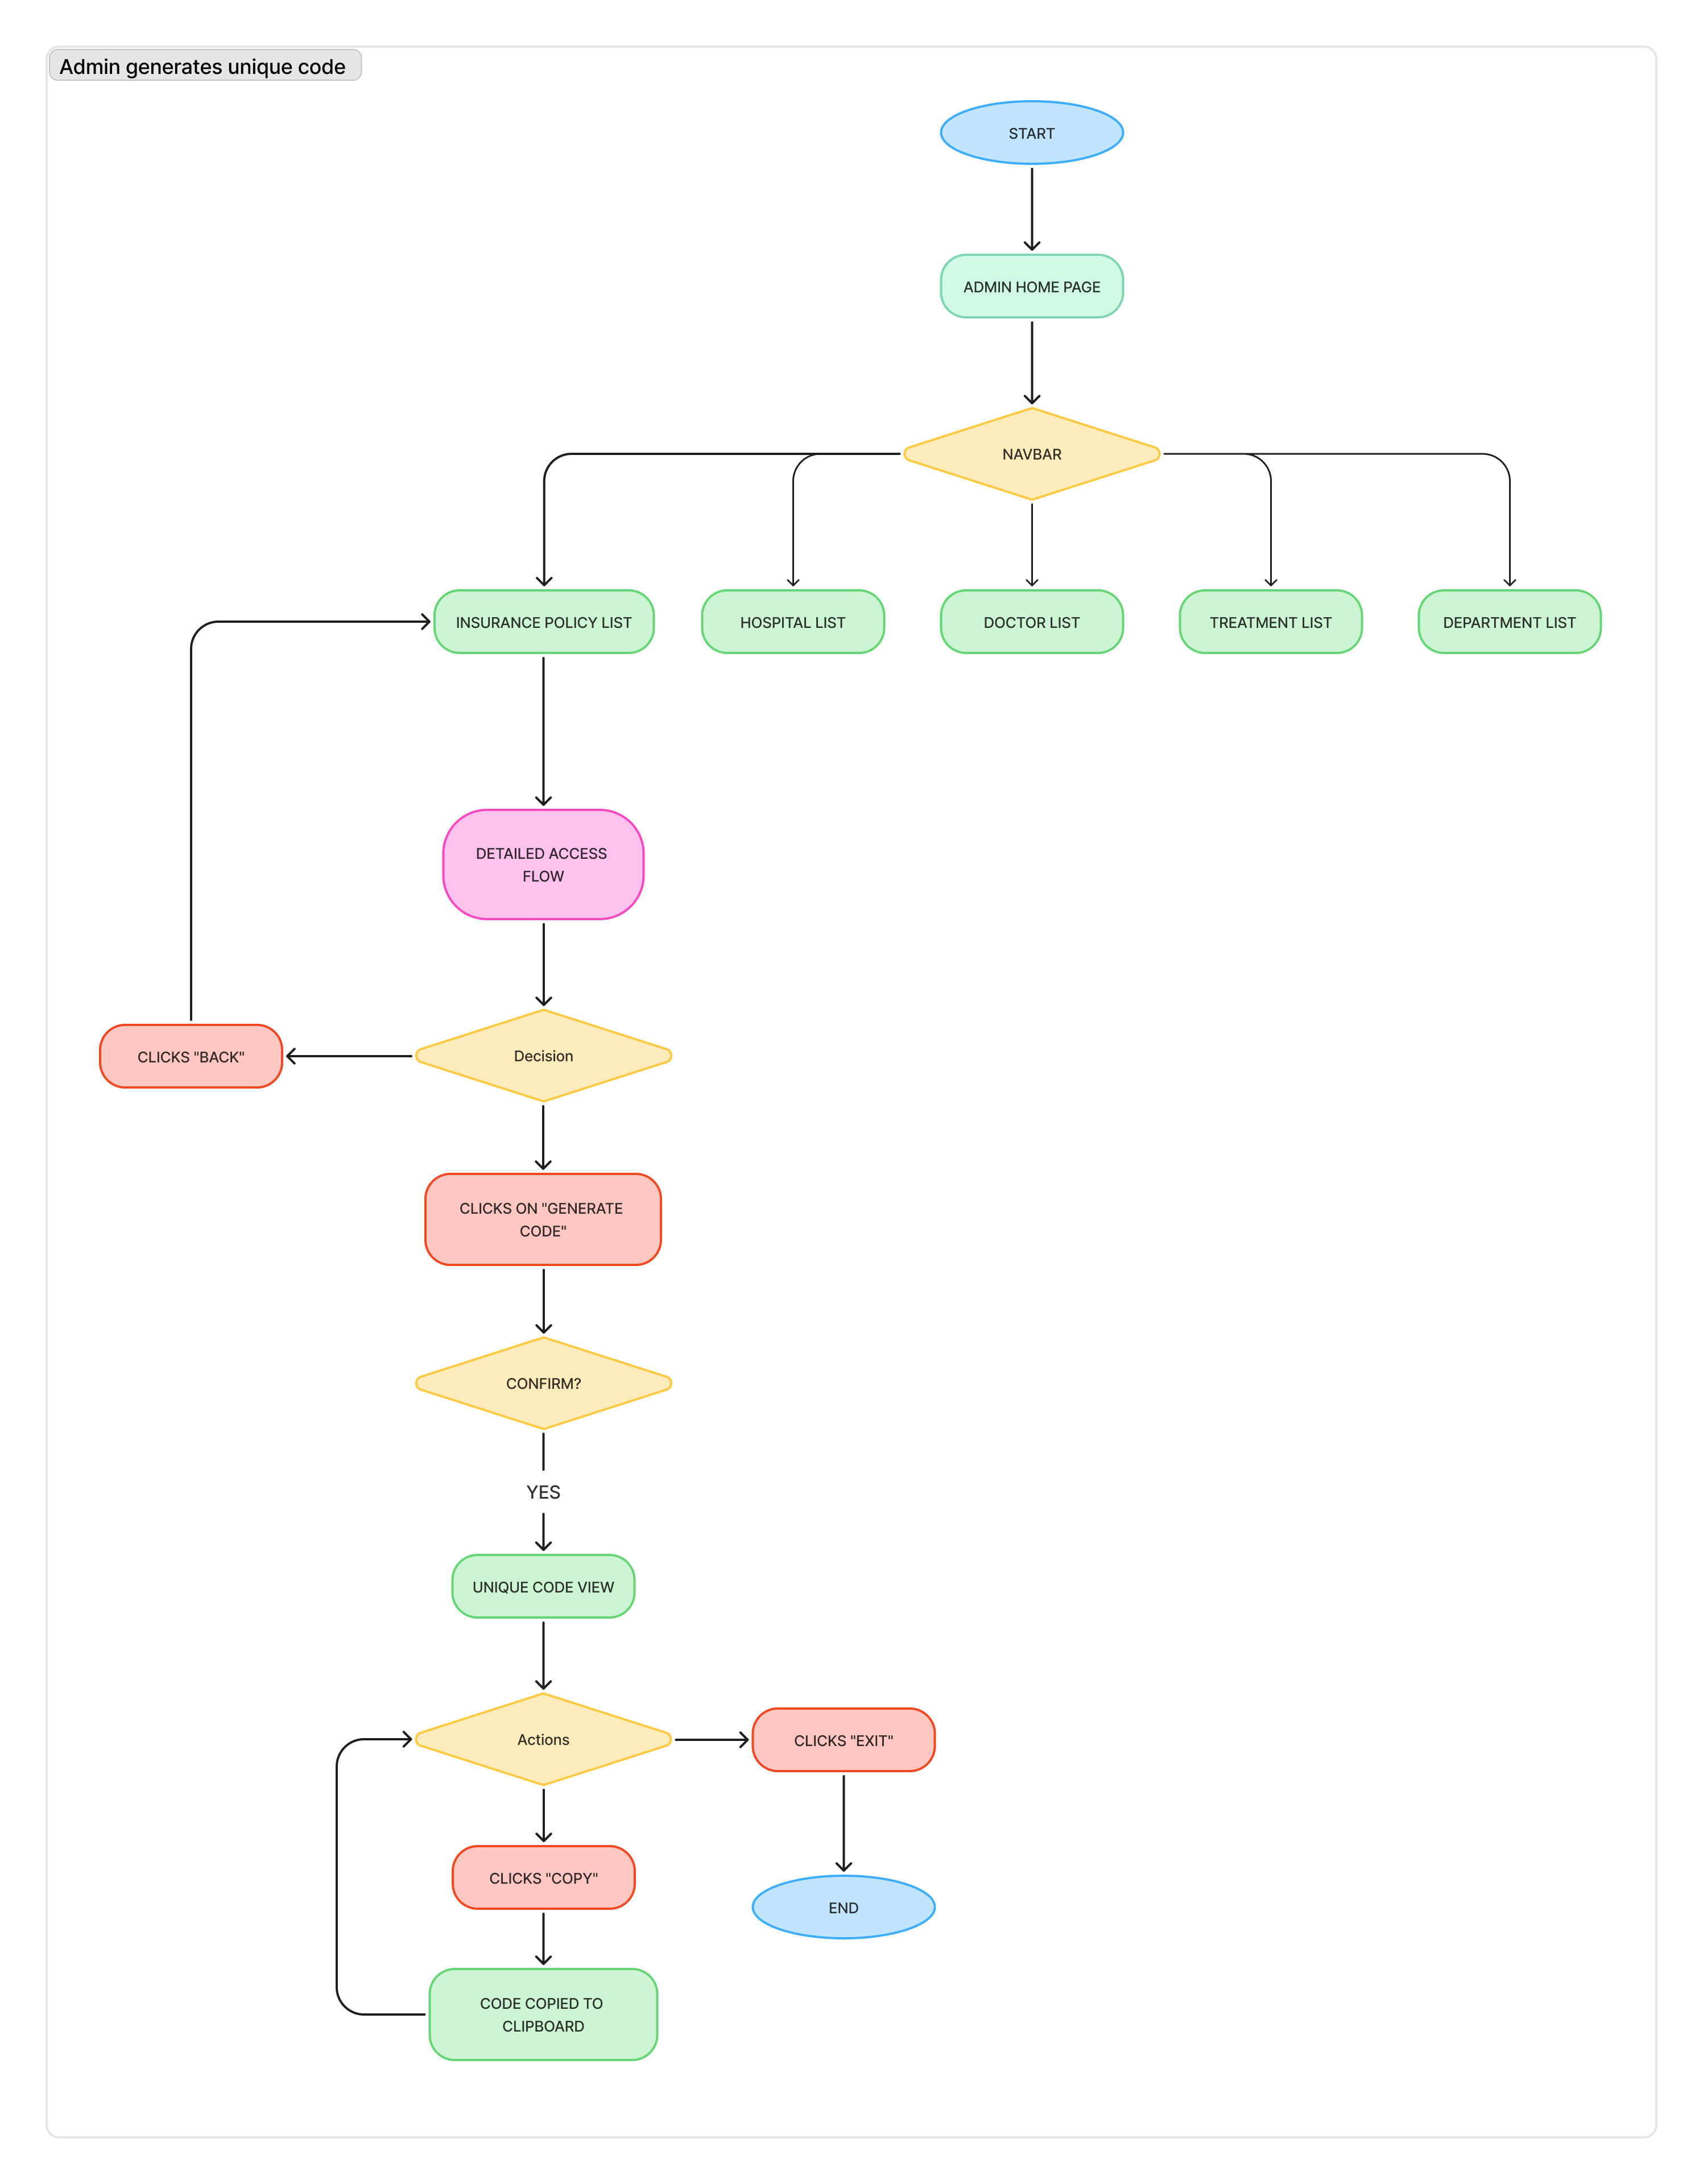
\includegraphics[width=0.8\textwidth]{User_Flows/GenerateUniqueCode.png}
        \captionof{figure}{User flow regarding Generate Unique Code}
    \end{center}
    %\begin{itemize}   
    %\end{itemize}
\end{minipage}
\vspace{3em}

\begin{minipage}{\textwidth}
    \phantomsection
    \subsection{UF12. Patient - Registration and Validation}
    \label{UF12}
    The following user flow shows the process of Patient registration and validation. UC23 is implemented.
    It refers to use case \textbf{UC23}, and methods \textbf{register(userData), validateAccount(token)} from the class \textbf{Patient} of the class diagram.
    
    \begin{center}
        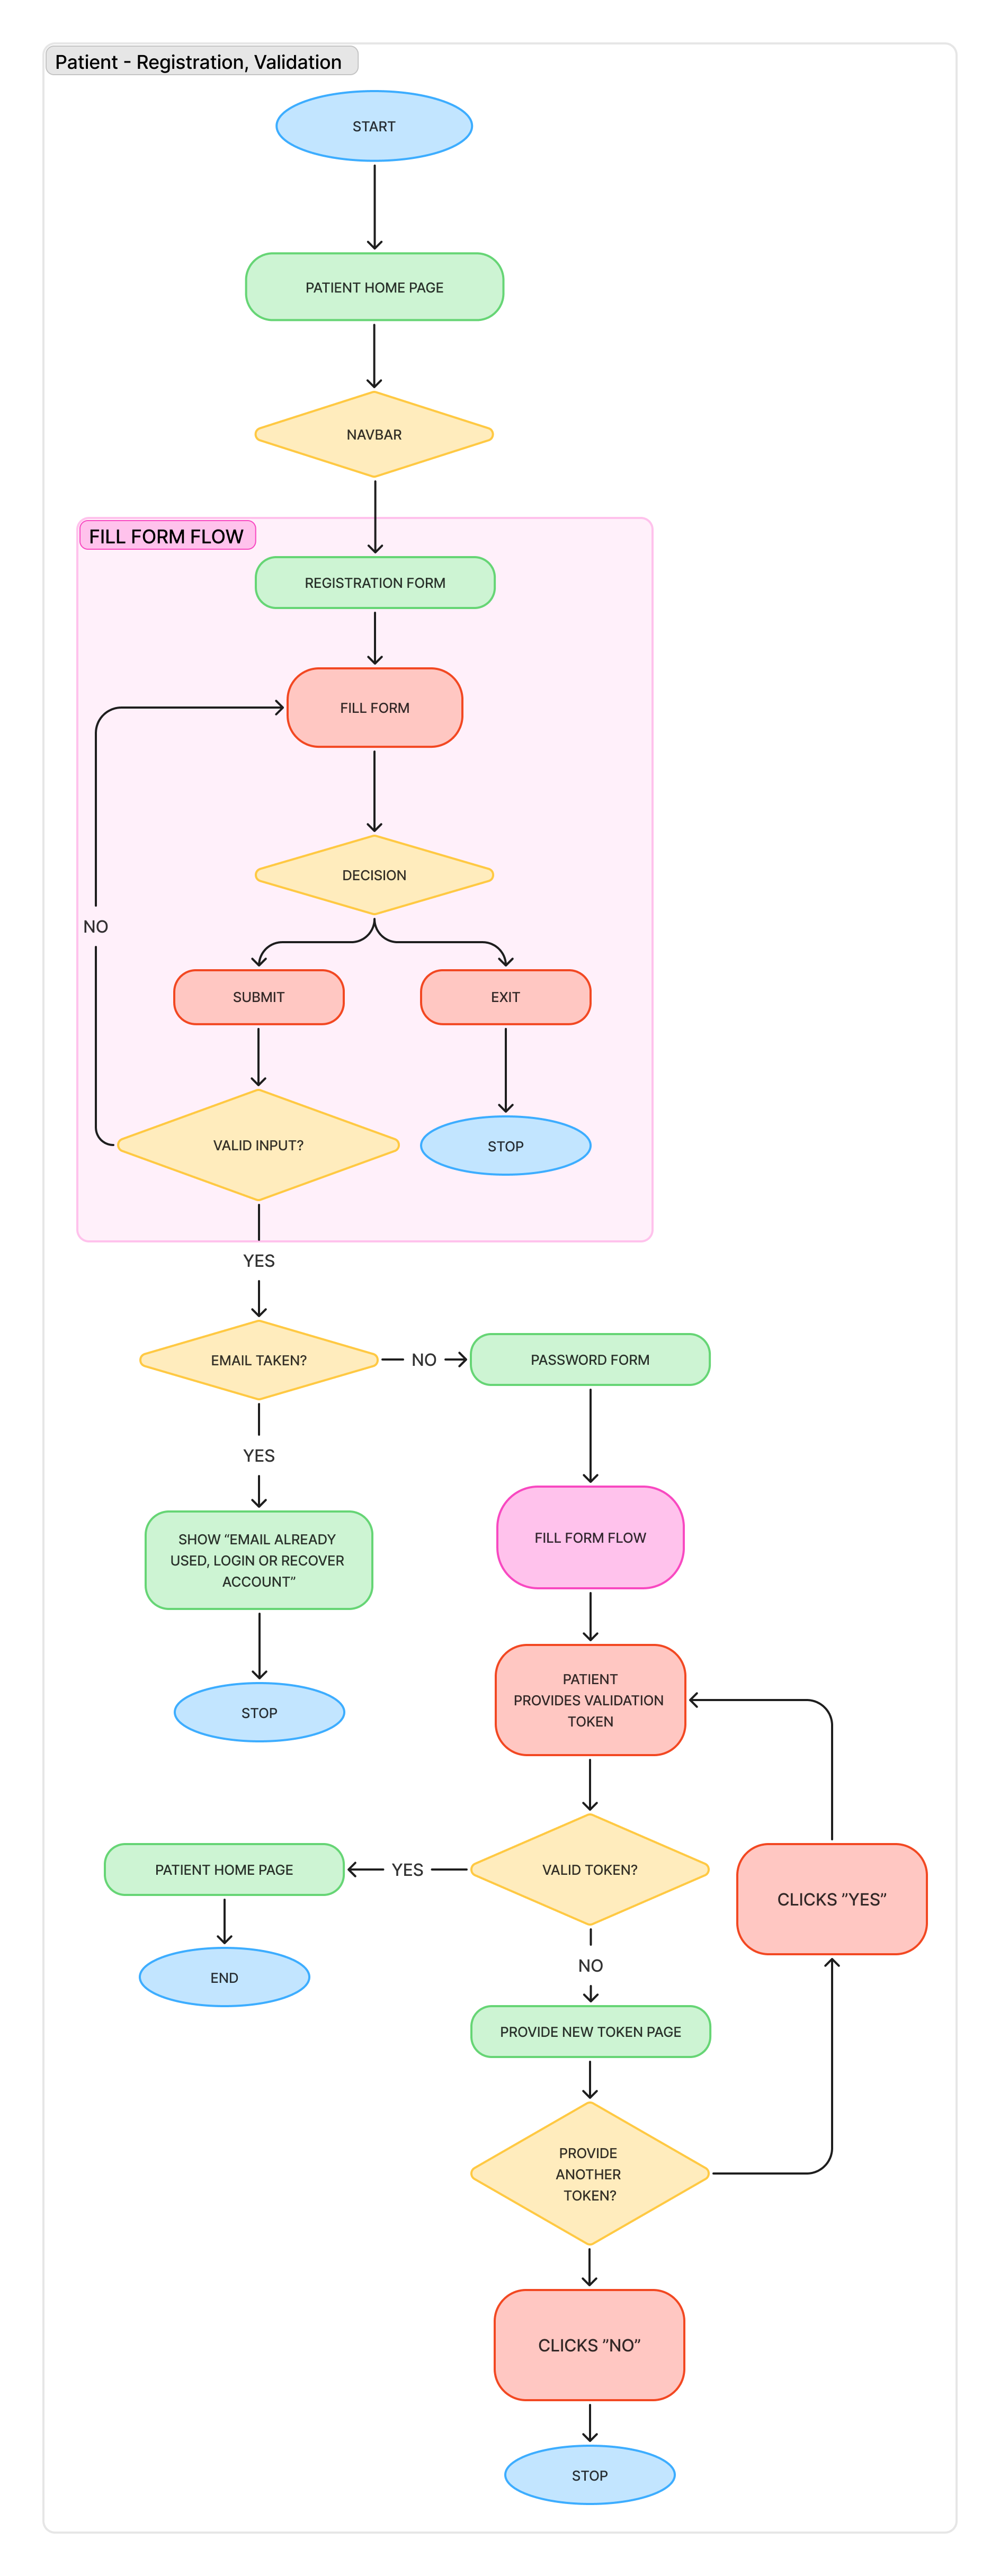
\includegraphics[width=8cm]{User_Flows/PatientRegistrationValidation.png}
        \captionof{figure}{User flow regarding Patient Registration and Validation}
    \end{center}
    %\begin{itemize}   
    %\end{itemize}
\end{minipage}
\vspace{3em}

\begin{minipage}{\textwidth}
    \phantomsection
    \subsection{UF13. Patient - Appointment Cancellation and Rescheduling}
    The following user flow shows the steps a patient takes to cancel and reschedule an appointment. UC10 is implemented, while UC29 is not.
    It refers to use cases \textbf{UC10, UC29}, and methods \textbf{cancel(), reschedule(newDateTime)} from the class \textbf{Appointment} of the class diagram.
    
    \begin{center}
        
\includegraphics[width=0.8\textwidth]{User_Flows/PatientCancellationRescheduling.png}
        \captionof{figure}{User flow regarding Patient Appointment Cancellation and Rescheduling}
    \end{center}
    %\begin{itemize}   
    %\end{itemize}
\end{minipage}
\vspace{3em}

\begin{minipage}{\textwidth}
    \phantomsection
    \subsection{UF14. Patient - Appointment Booking and Payment}
    The following user flow shows the steps a patient takes to book and pay an appointment. UC27 is implemented while UC32 and UC35 are not.
    It refers to use cases \textbf{UC27, UC32, UC35}, and methods \textbf{Appointment.book(treatment,hospital,datetime), Payment.pay(paymentData)} from the classes \textbf{Appointment, Payment} of the class diagram.
    
    \begin{center}
        
\includegraphics[width=0.8\textwidth]{User_Flows/AppointmentBookingPayment.png}
        \captionof{figure}{User flow regarding Patient Appointment Booking and Payment}
    \end{center}
    %\begin{itemize}   
    %\end{itemize}
\end{minipage}
\vspace{3em}

\begin{minipage}{\textwidth}
    \phantomsection
    \subsection{UF15. Patient - Register Insurance Policy via unique code}
    The following user flow shows the steps a patient takes to add an insurance policy to their profile via unique code. UC36 is not implemented.
    It refers to use case \textbf{UC36}, and methods \textbf{registerInsurance(code)} from the class \textbf{Patient} of the class diagram.
    
    \begin{center}
        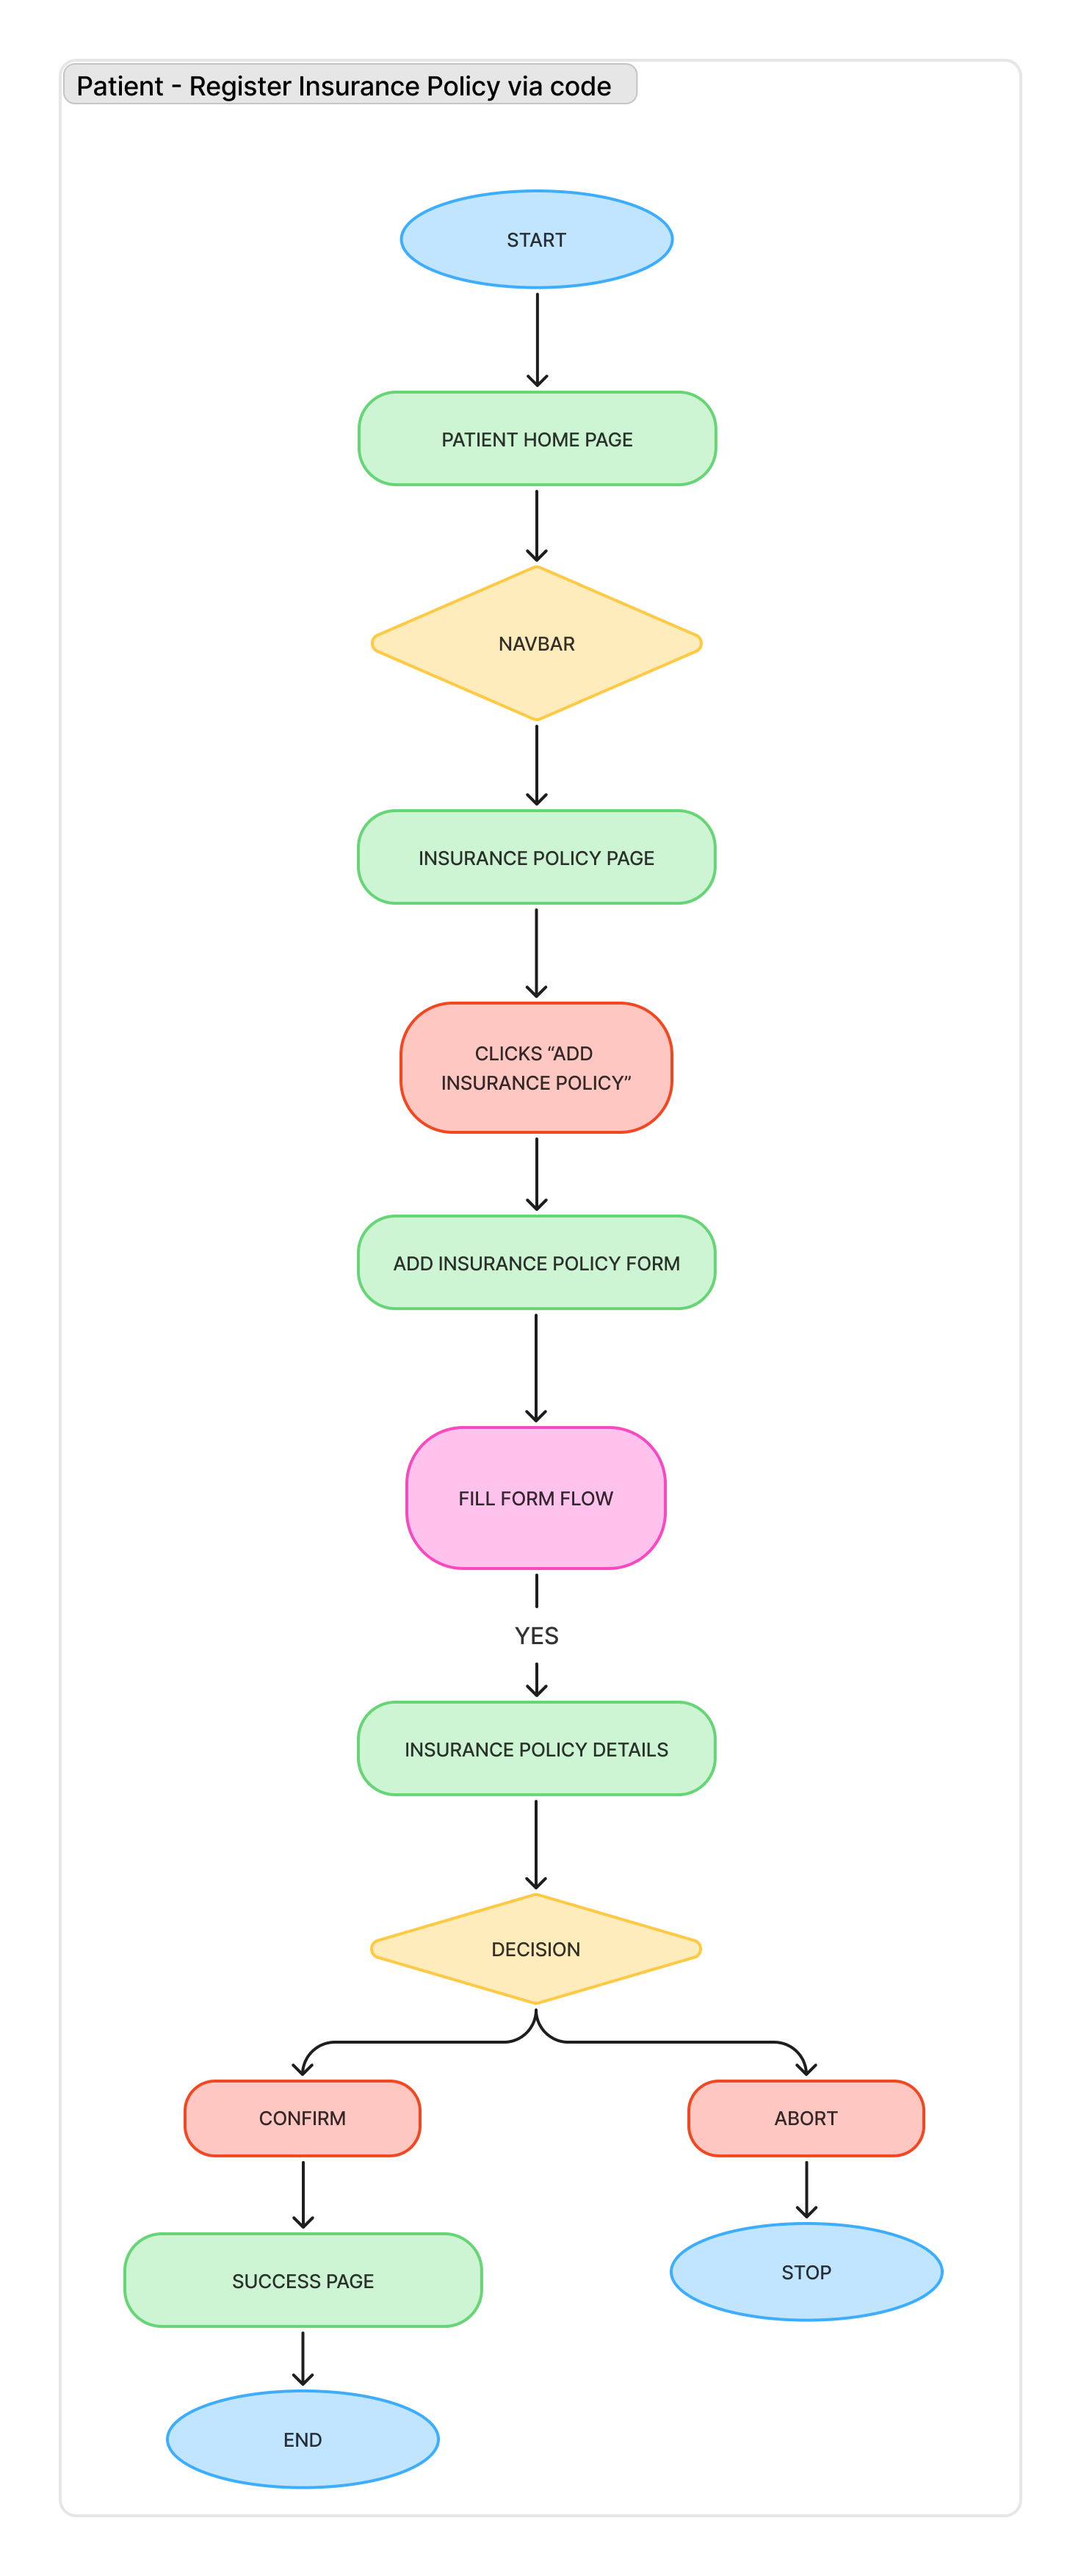
\includegraphics[width=0.5\textwidth]{User_Flows/PatientRegisterPolicy.png}
        \captionof{figure}{User flow regarding Patient Register Insurance Policy via unique code}
    \end{center}
    %\begin{itemize}   
    %\end{itemize}
\end{minipage}
\vspace{3em}

\begin{minipage}{\textwidth}
    \phantomsection
    \subsection{UF16. Patient - Medical Record and Prescriptions consultation}
    \label{UF16}
    The following user flow shows the steps a patient takes to view their medical record and prescriptions in detail. UC38, UC39 and UC40 are implemented.
    It refers to use cases \textbf{UC38, UC39, UC40}, and methods \textbf{Patient.getPrescriptions(), Prescription.getDetails(), Patient.getMedicalRecord()} from the classes \textbf{Patient, Prescription} of the class diagram.
    
    \begin{center}
        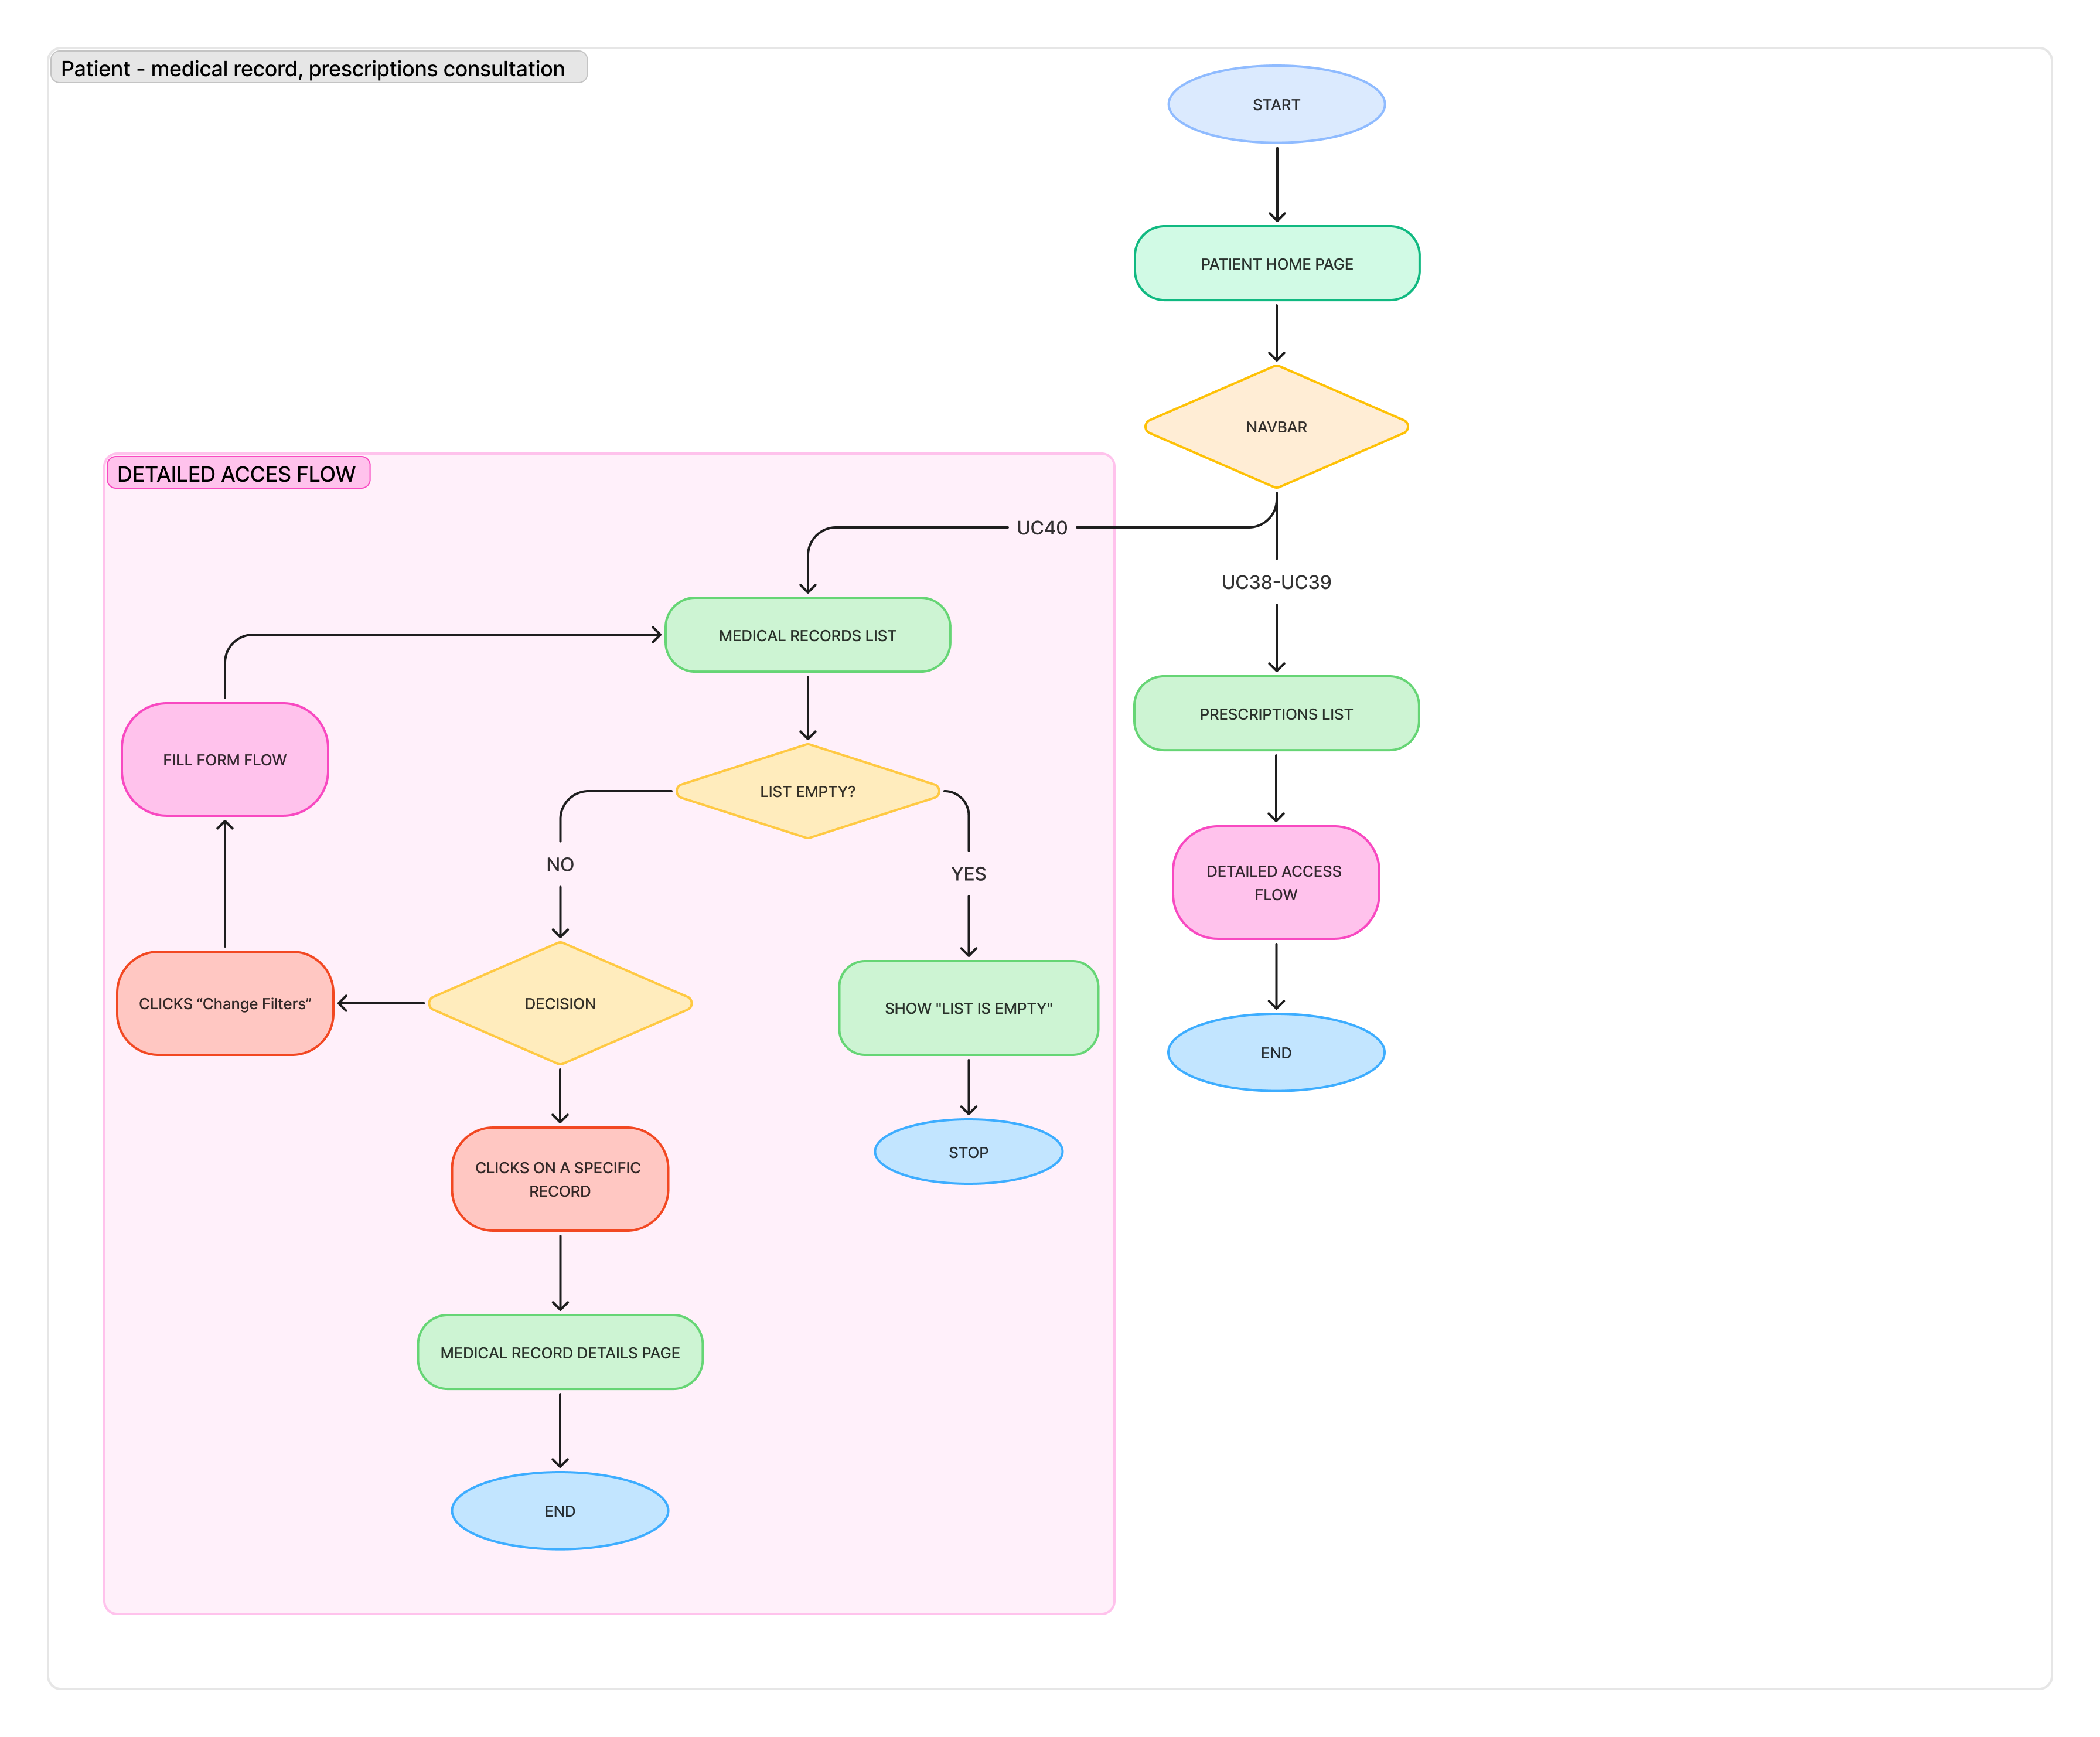
\includegraphics[width=0.9\textwidth]{User_Flows/PatientMedicalRecordPrescriptionExemptions.png}
        \captionof{figure}{User flow regarding Patient Medical Record and Prescriptions consultation}
    \end{center}
    %\begin{itemize}   
    %\end{itemize}
\end{minipage}
\vspace{3em}

\begin{minipage}{\textwidth}    
    \phantomsection
    \subsection{UF17. Doctor - Access Patient's Medical Record, Chronological Report}
    The following user flow shows the steps a doctor takes to access a patient's medical records and to consult their own chronological report. UC42 and UC43 are implemented.
    It refers to use cases \textbf{UC42, UC43}, and methods \textbf{accessPatientRecord(fiscalCode),viewChronologicalReport()} from the class \textbf{Doctor} of the class diagram.
    
    \begin{center}
        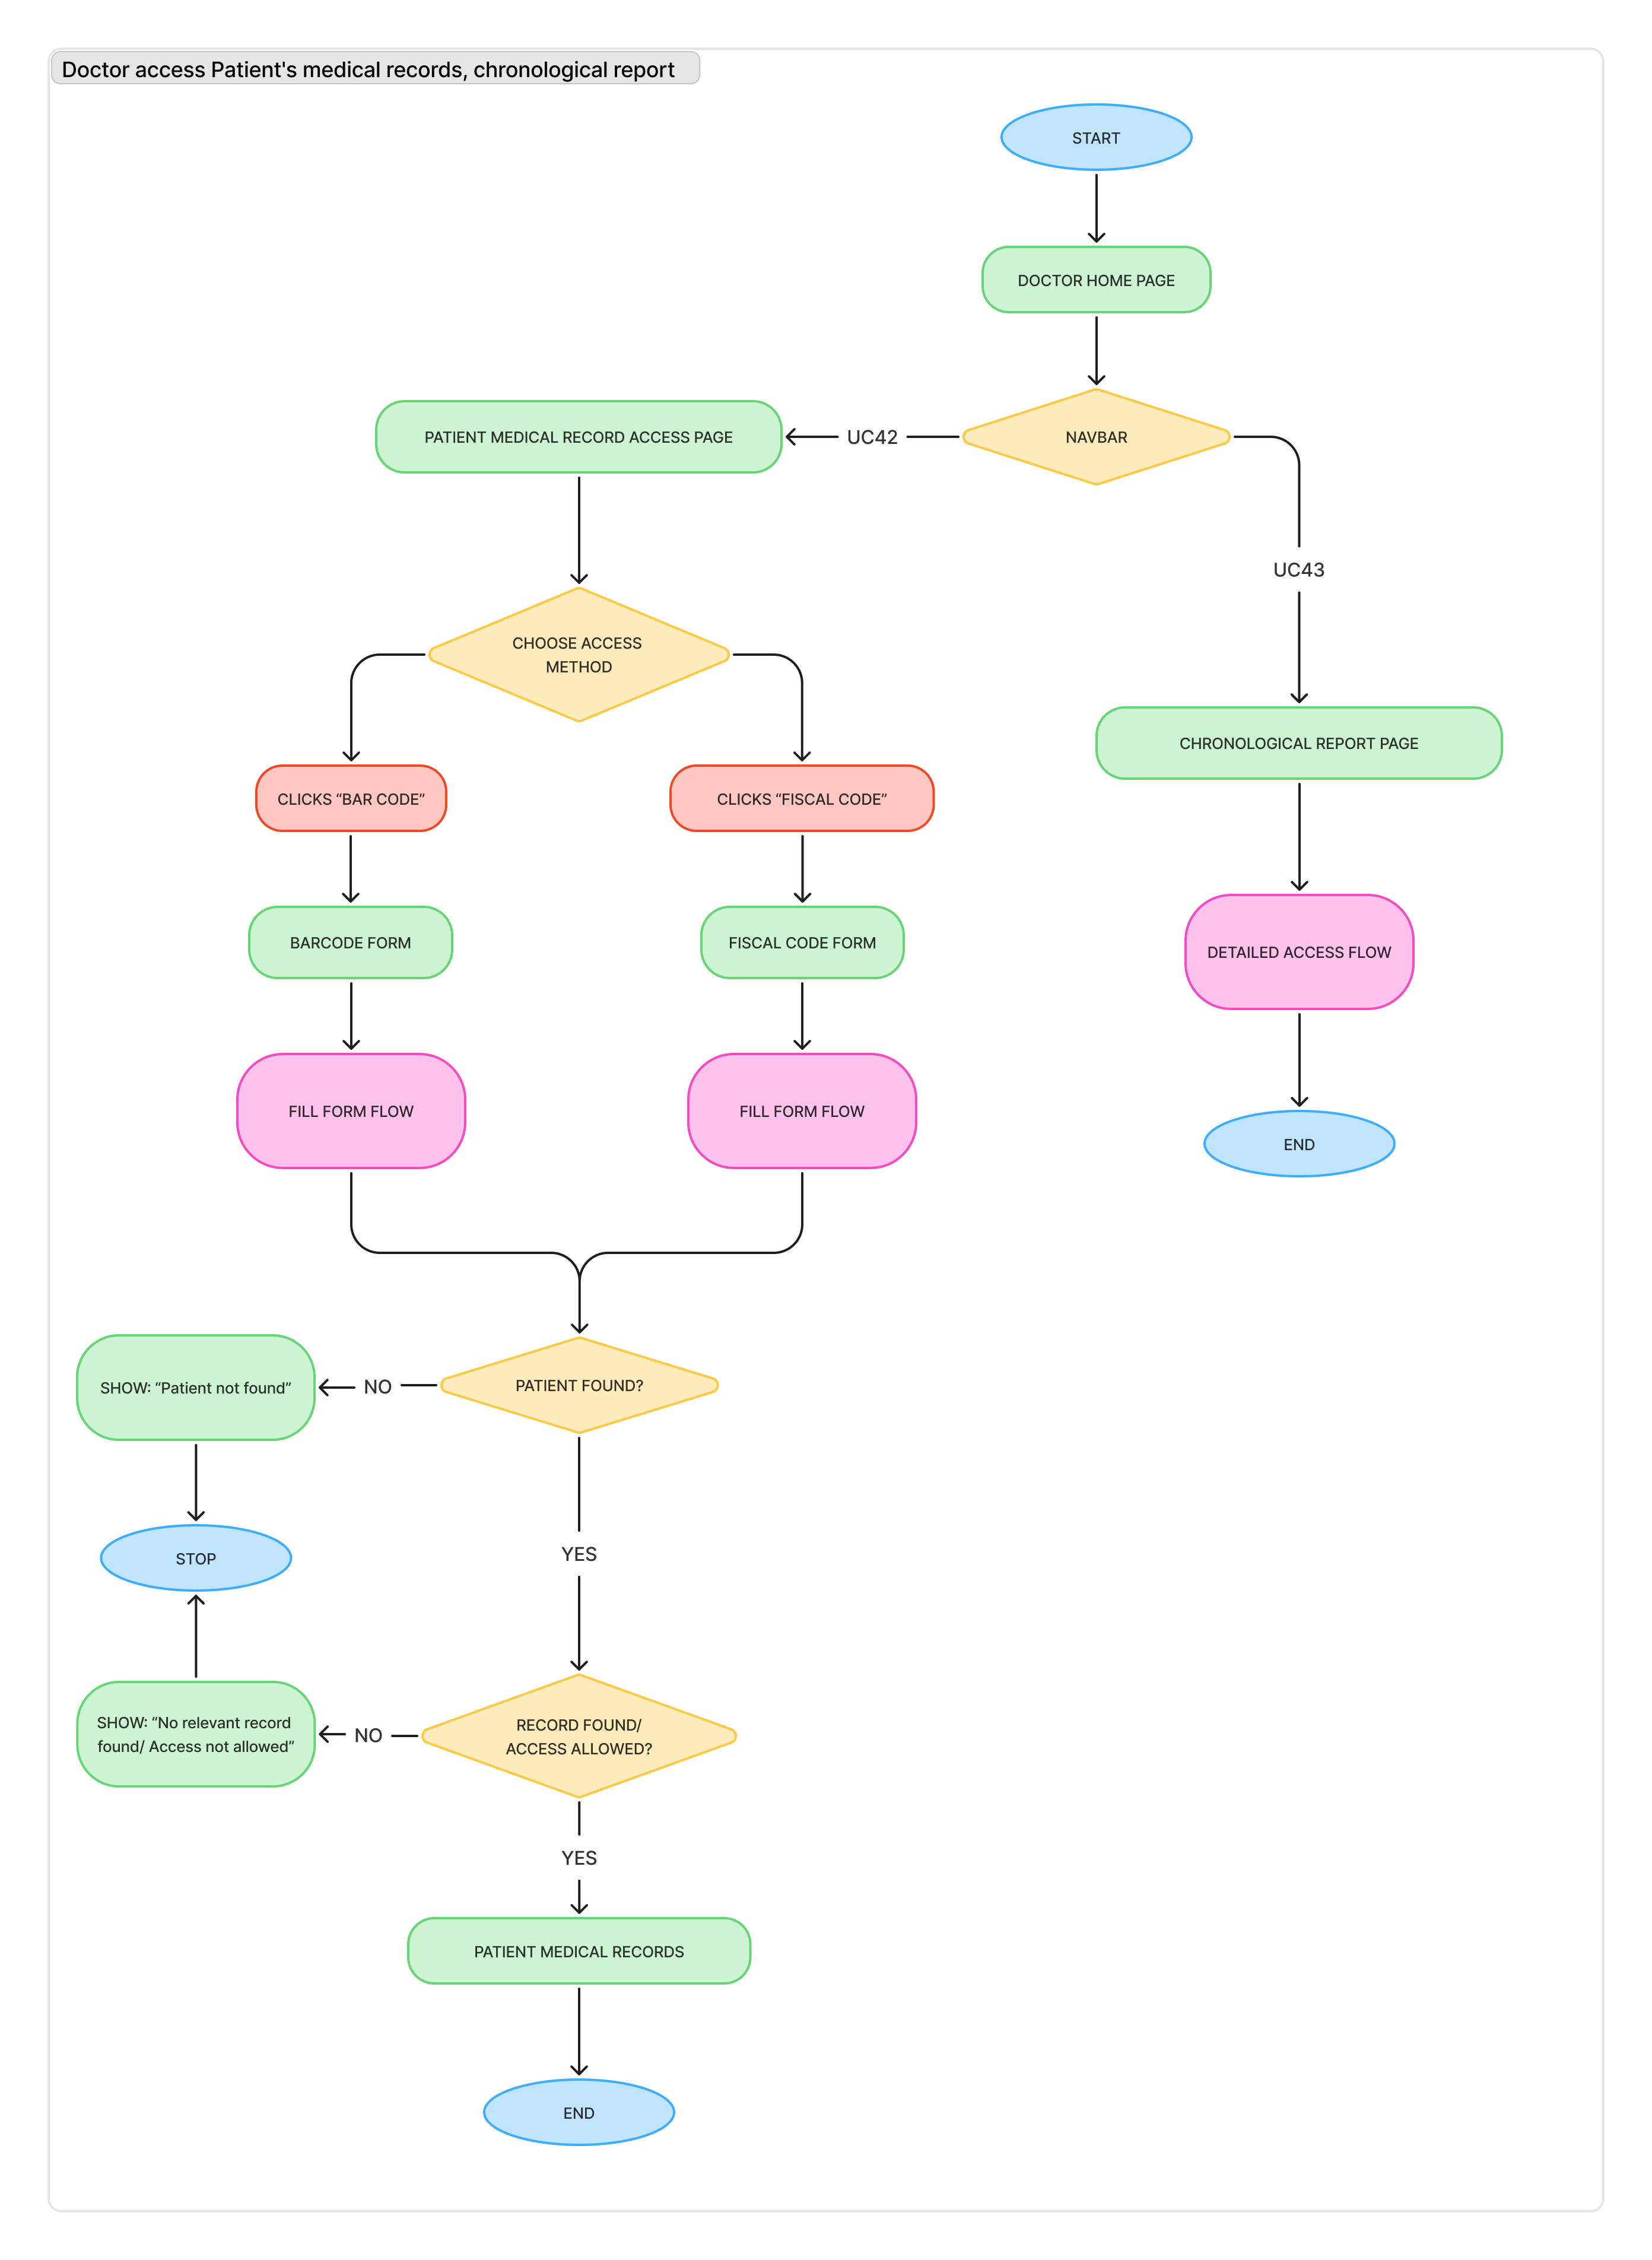
\includegraphics[width=0.7\textwidth]{User_Flows/DoctorMedicalRecordReport.png}
        \captionof{figure}{User flow regarding Doctor Access Patient's Medical Record, Chronological Report}
    \end{center}
    %\begin{itemize}   
    %\end{itemize}
\end{minipage}
\vspace{3em}

\begin{minipage}{\textwidth}
    \phantomsection
    \subsection{UF18. Doctor - Upload Prescriptions, Exemptions and Exam Results}
    The following user flow shows the steps a doctor takes to upload prescriptions, exemptions and exam results to a patient's profile. UC3 and UC4 are implemented.
    It refers to use cases \textbf{UC3, UC4}, and methods \textbf{Prescription.create(prescriptionData), Exemption.create(exemptionData), Examination.create(examinationData)} from the classes \textbf{Prescription, Exemption, Examination} of the class diagram.
    
    \begin{center}
        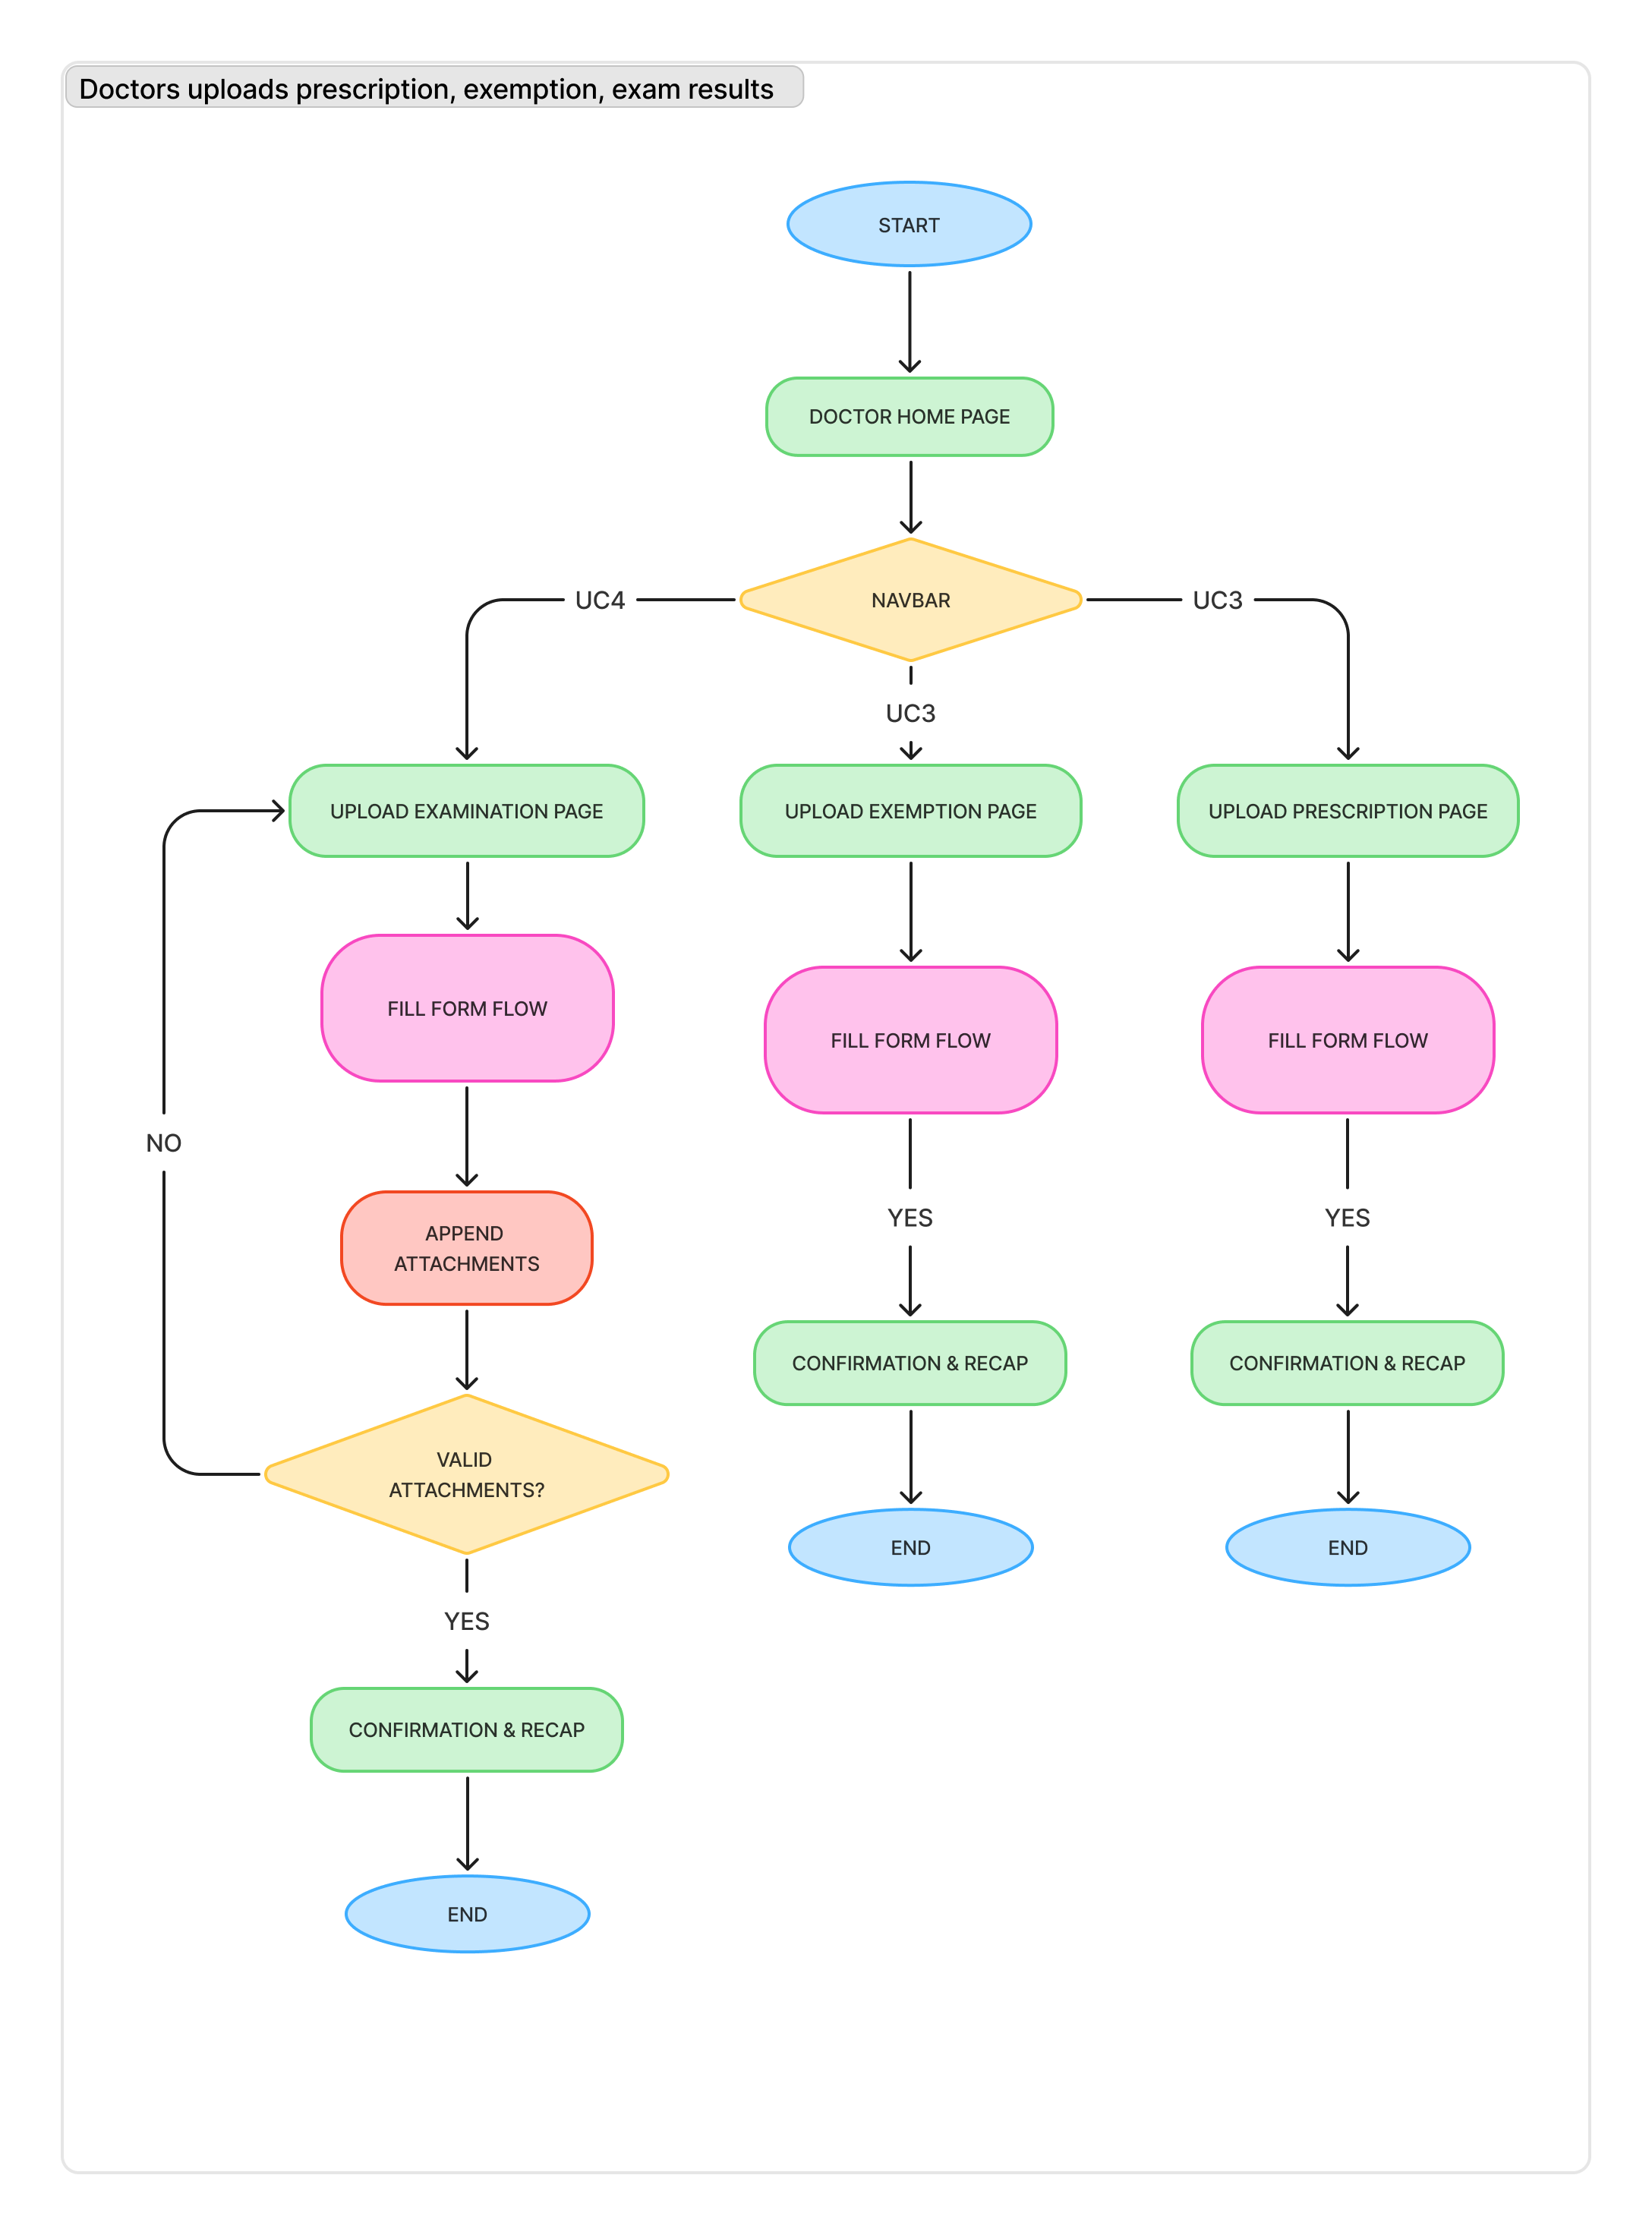
\includegraphics[width=0.9\textwidth]{User_Flows/DoctorUploads.png}
        \captionof{figure}{User flow regarding Doctor Upload Prescriptions, Exemptions and Exam Results}
    \end{center}
    %\begin{itemize}   
    %\end{itemize}
\end{minipage}
\vspace{3em}

\begin{minipage}{\textwidth}
    \phantomsection
    \subsection{UF19. Doctor - Cancel Appointment}
    The following user flow shows the steps a doctor takes to cancel one of their booked examinations. UC11 is implemented.
    It refers to use case \textbf{UC11}, and methods \textbf{cancel(reason : String)} from the class \textbf{Appointment} of the class diagram.
    
    \begin{center}
        
\includegraphics[width=0.8\textwidth,height=0.7\textheight,keepaspectratio]{User_Flows/DoctorAppointmentCancellation.png}
        \captionof{figure}{User flow regarding Doctor Appointment Cancellation}
    \end{center}
    %\begin{itemize}   
    %\end{itemize}
\end{minipage}
\vspace{3em}

\begin{minipage}{\textwidth}
    \phantomsection
    \subsection{UF20. Head of Department - Management Operations}
    The following user flow shows the steps a head of department takes to configure their department's services, capacity and doctor's workshifts. UC17, UC21 and UC44 are not implemented.
    It refers to use cases \textbf{UC17, UC21, UC44}, and methods \textbf{updateDepartmentTreatments(newTreatments), configureDepartmentCapacity(newCapacity),  setShiftPattern(Doctor, Shifts)} from the class \textbf{Head of Department} of the class diagram.
    
    \begin{center}
        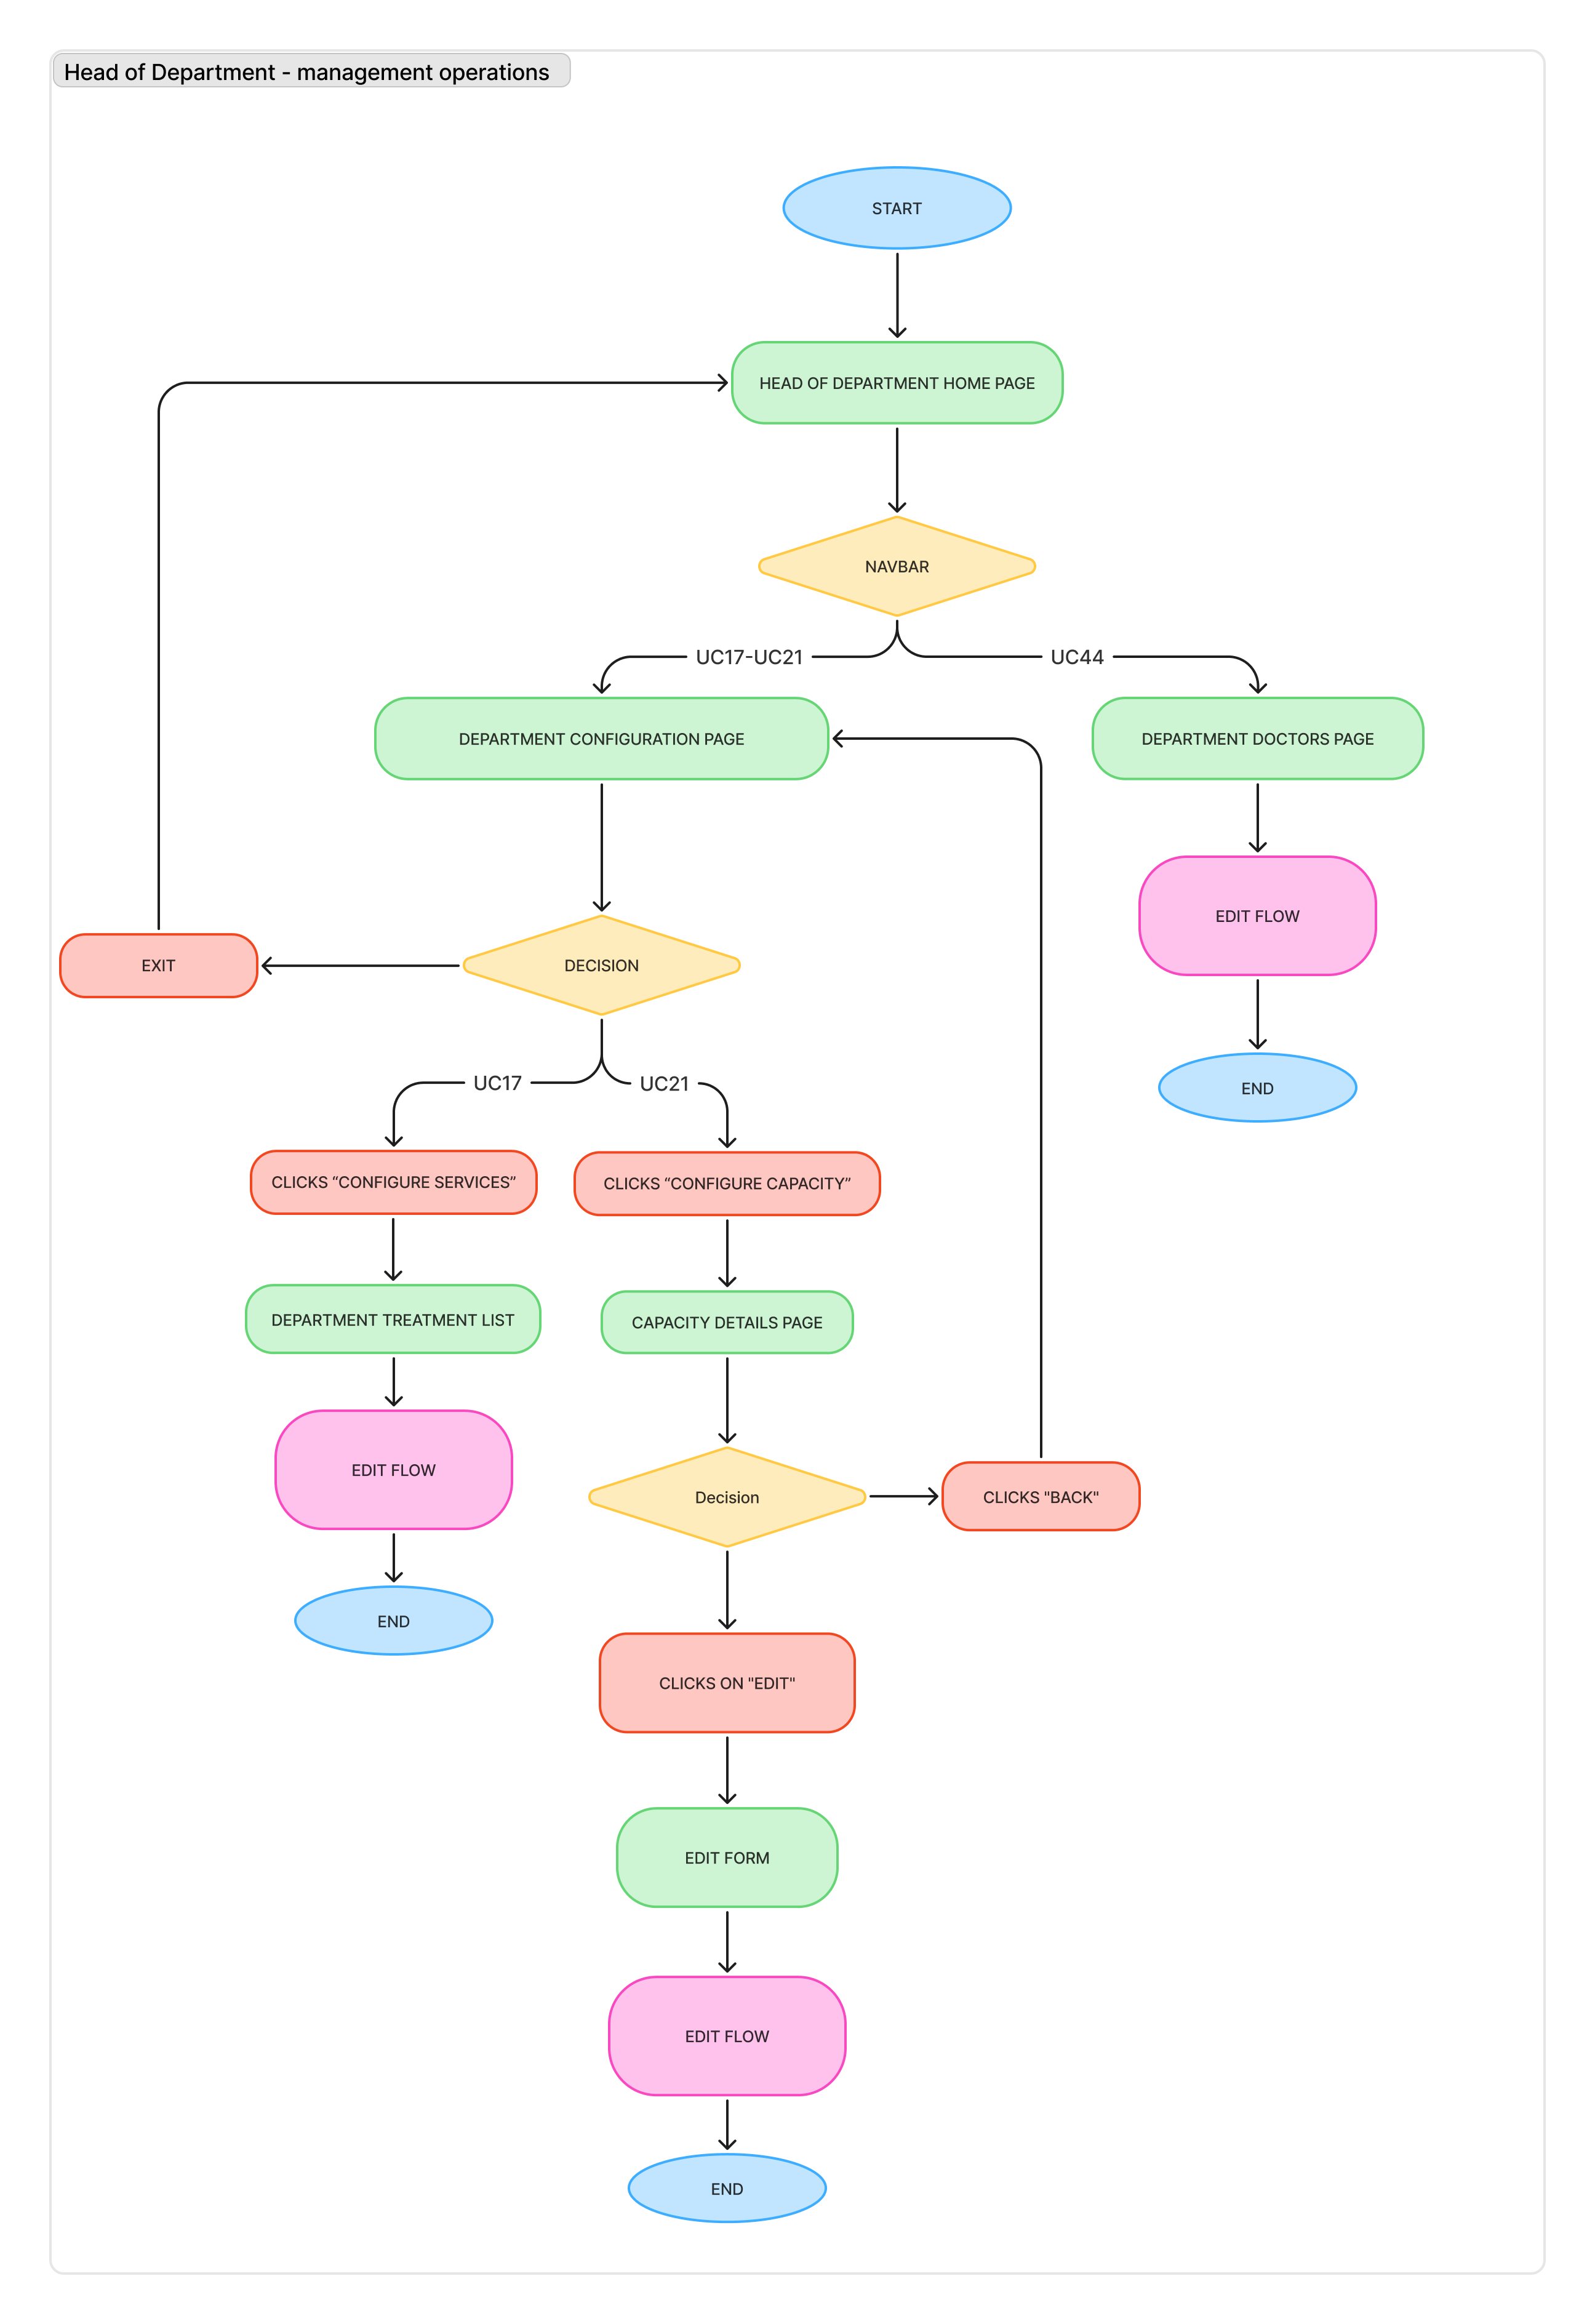
\includegraphics[width=0.8\textwidth]{User_Flows/DepartmentManagement.png}
        \captionof{figure}{User flow regarding Head of Department Management Operations}
    \end{center}
    %\begin{itemize}   
    %\end{itemize}
\end{minipage}
\vspace{3em}

\begin{minipage}{\textwidth}
    \phantomsection
    \subsection{UF21. Head of Department - Cancel Department Appointments}
    The following user flow shows the steps a head of department takes to cancel their department's booked appointments. UC11 is implemented.
    It refers to use case \textbf{UC11}, and methods \textbf{Appointment.cancel(reason)} from the class \textbf{Appointment} of the class diagram.

    \begin{center}
        
\includegraphics[width=0.9\textwidth, height=0.75\textheight, keepaspectratio]{User_Flows/DepartmentAppointmentCancellation.png}
        \captionof{figure}{User flow regarding Head of Department Cancel Department Appointments}
    \end{center}
    \end{minipage}
\vspace{3em}

\vspace{3em}

\begin{minipage}{\textwidth}
    \phantomsection
    \subsection{UF22. Head of Hospital - Insurances' Debt Management}
    The following user flow shows the steps a head of hospital takes to consult the insurances' debts owed to the hospital and register payments from insurance companies. UC18, UC19 and UC20 are not implemented.
    It refers to use cases \textbf{UC18, UC19, UC20}, and methods \textbf{Hospital.getInsuranceDebt(), OutstandingDebt.getHistory(), OutstandingDebt.settle(amount)} from the classes \textbf{Hospital, OutstandingDebt} of the class diagram.
    
    \begin{center}
        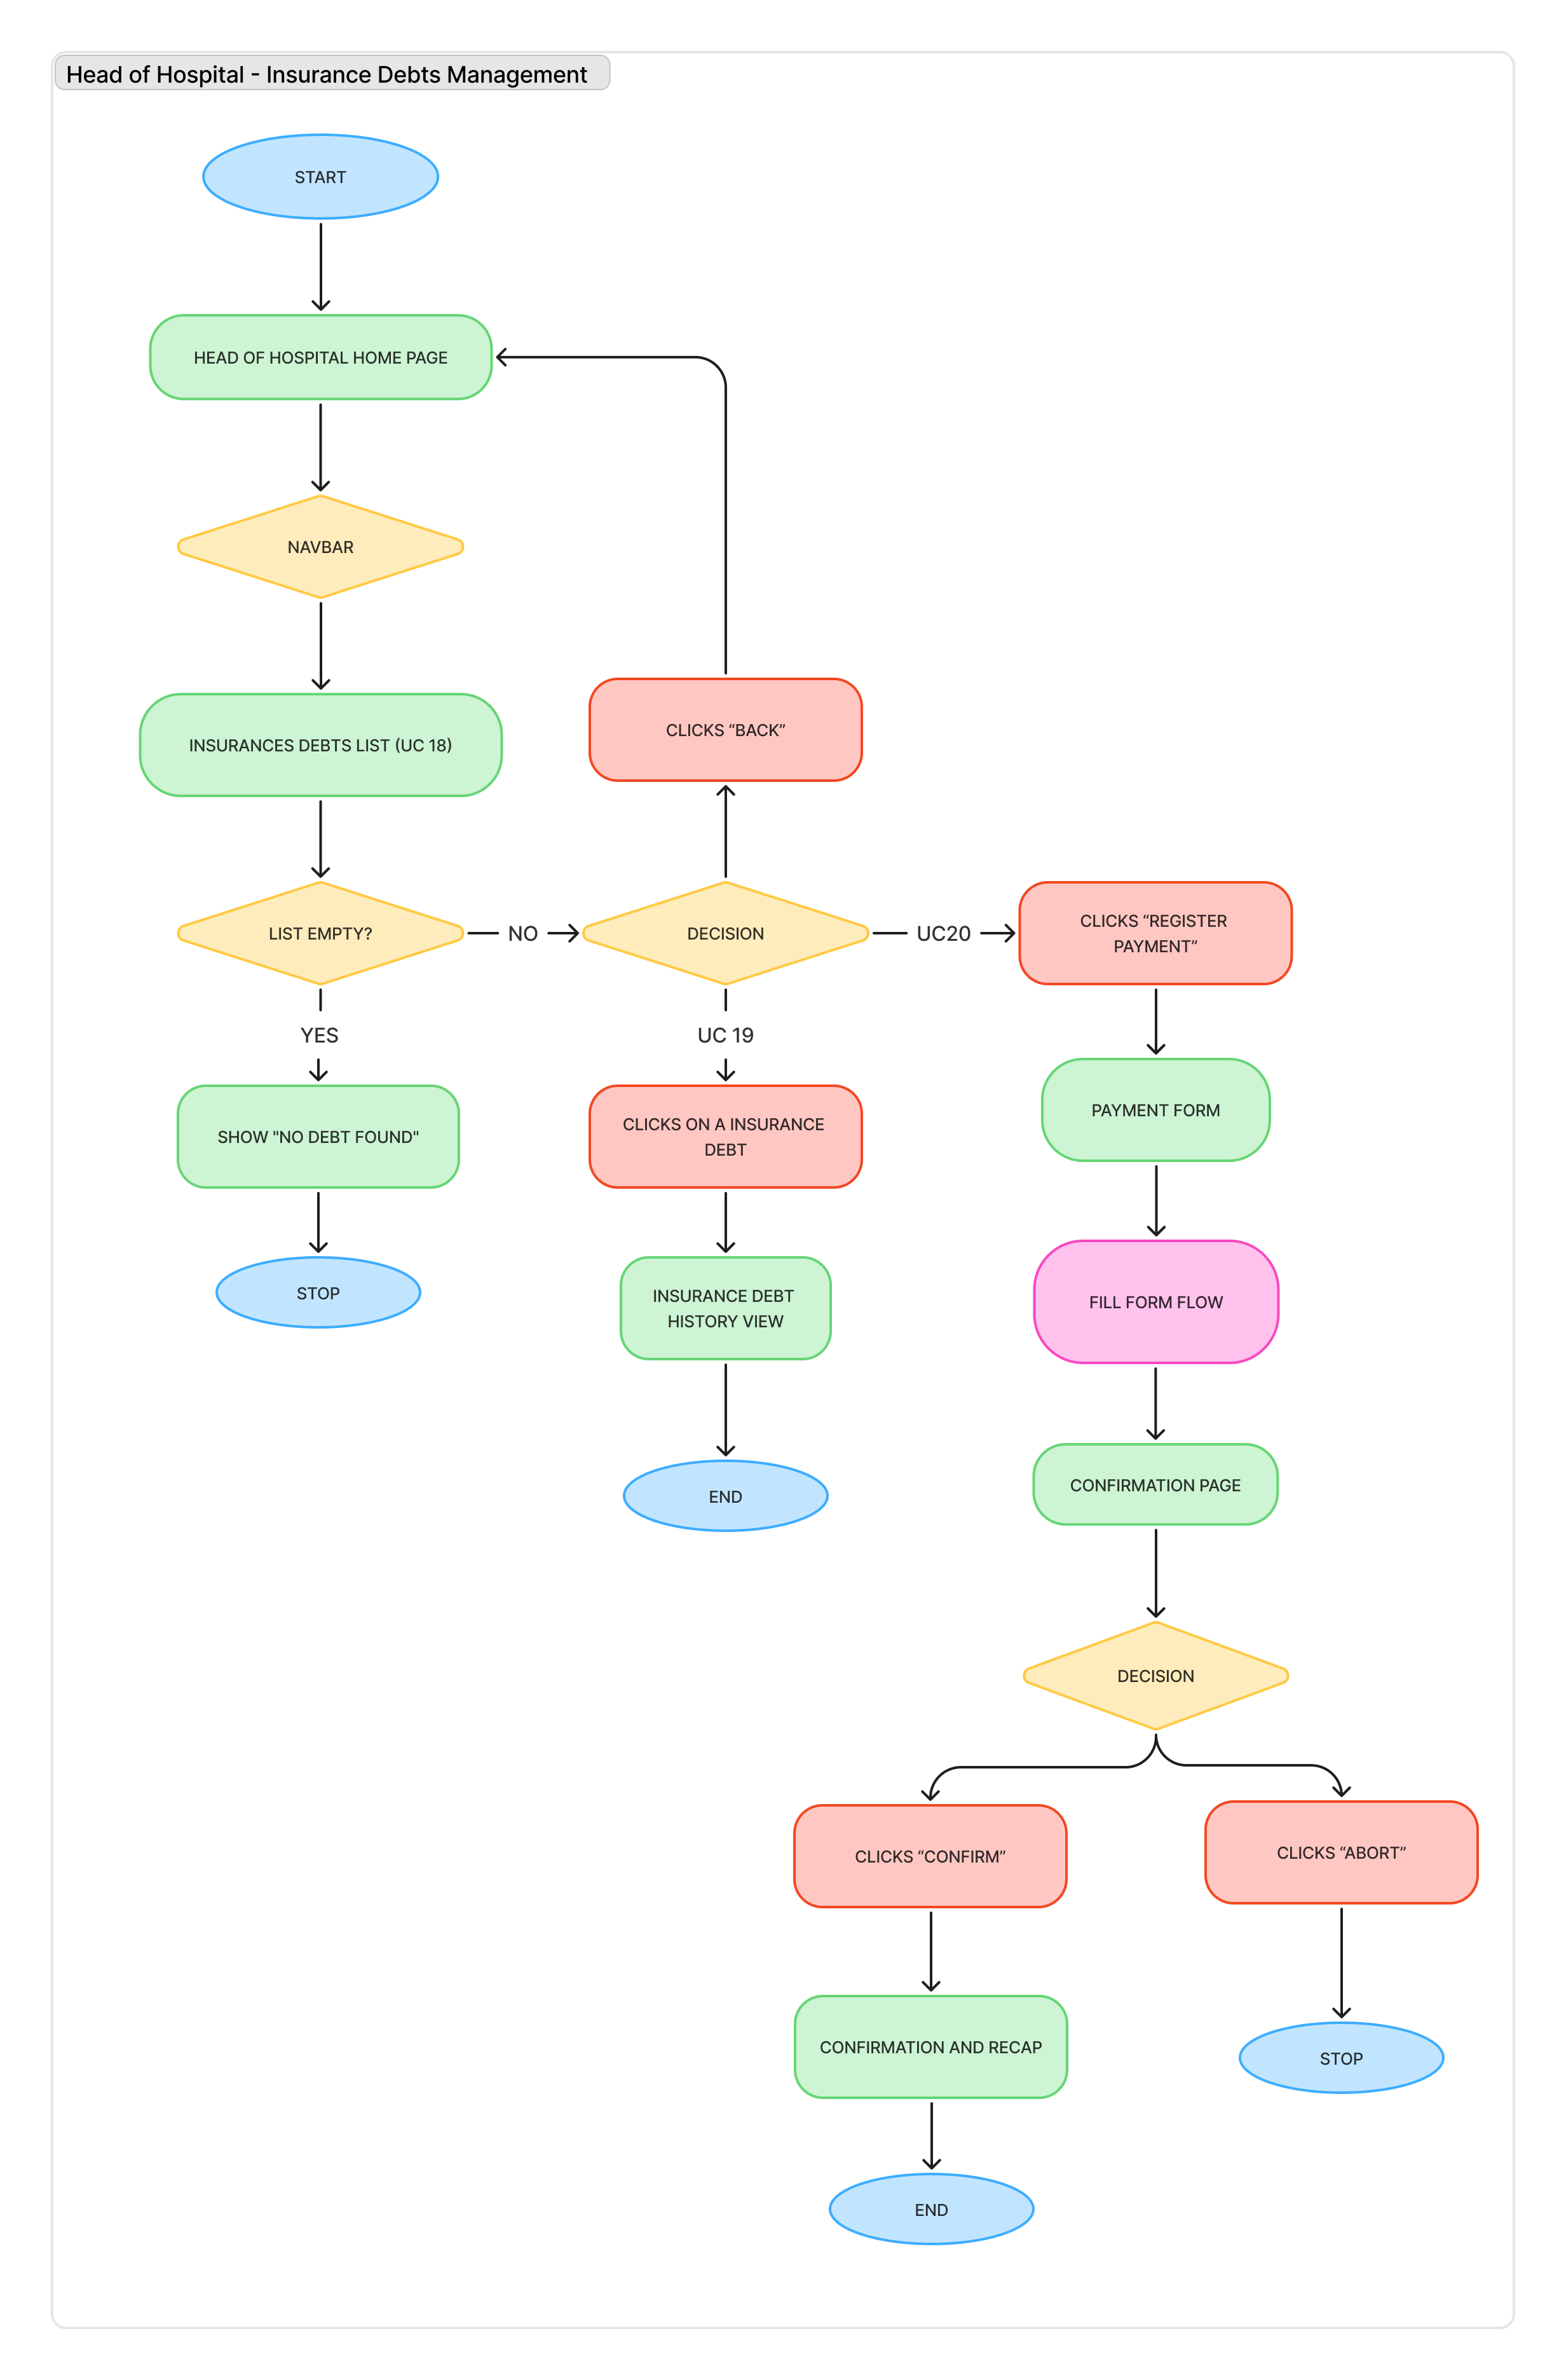
\includegraphics[width=0.8\textwidth]{User_Flows/HospitalDebtsManagement.png}
        \captionof{figure}{User flow regarding Head of Hospital Insurances' Debt Management}
    \end{center}    
    %\begin{itemize}   
    %\end{itemize}
\end{minipage}
\vspace{3em}

\begin{minipage}{\textwidth}
    \phantomsection
    \subsection{UF23. Head of Hospital - Department Assignments Management}
    The following user flow shows the steps a head of hospital takes to appoint a head of department and assign a doctor to a specific department. UC15 and UC16 are not implemented.
    It refers to use cases \textbf{UC15, UC16}, and methods \textbf{appointHeadOfDepartment(doctor, dept), allocateDoctors(doctors, dept)} from the class \textbf{Head of Hospital} of the class diagram.
    
    \begin{center}
        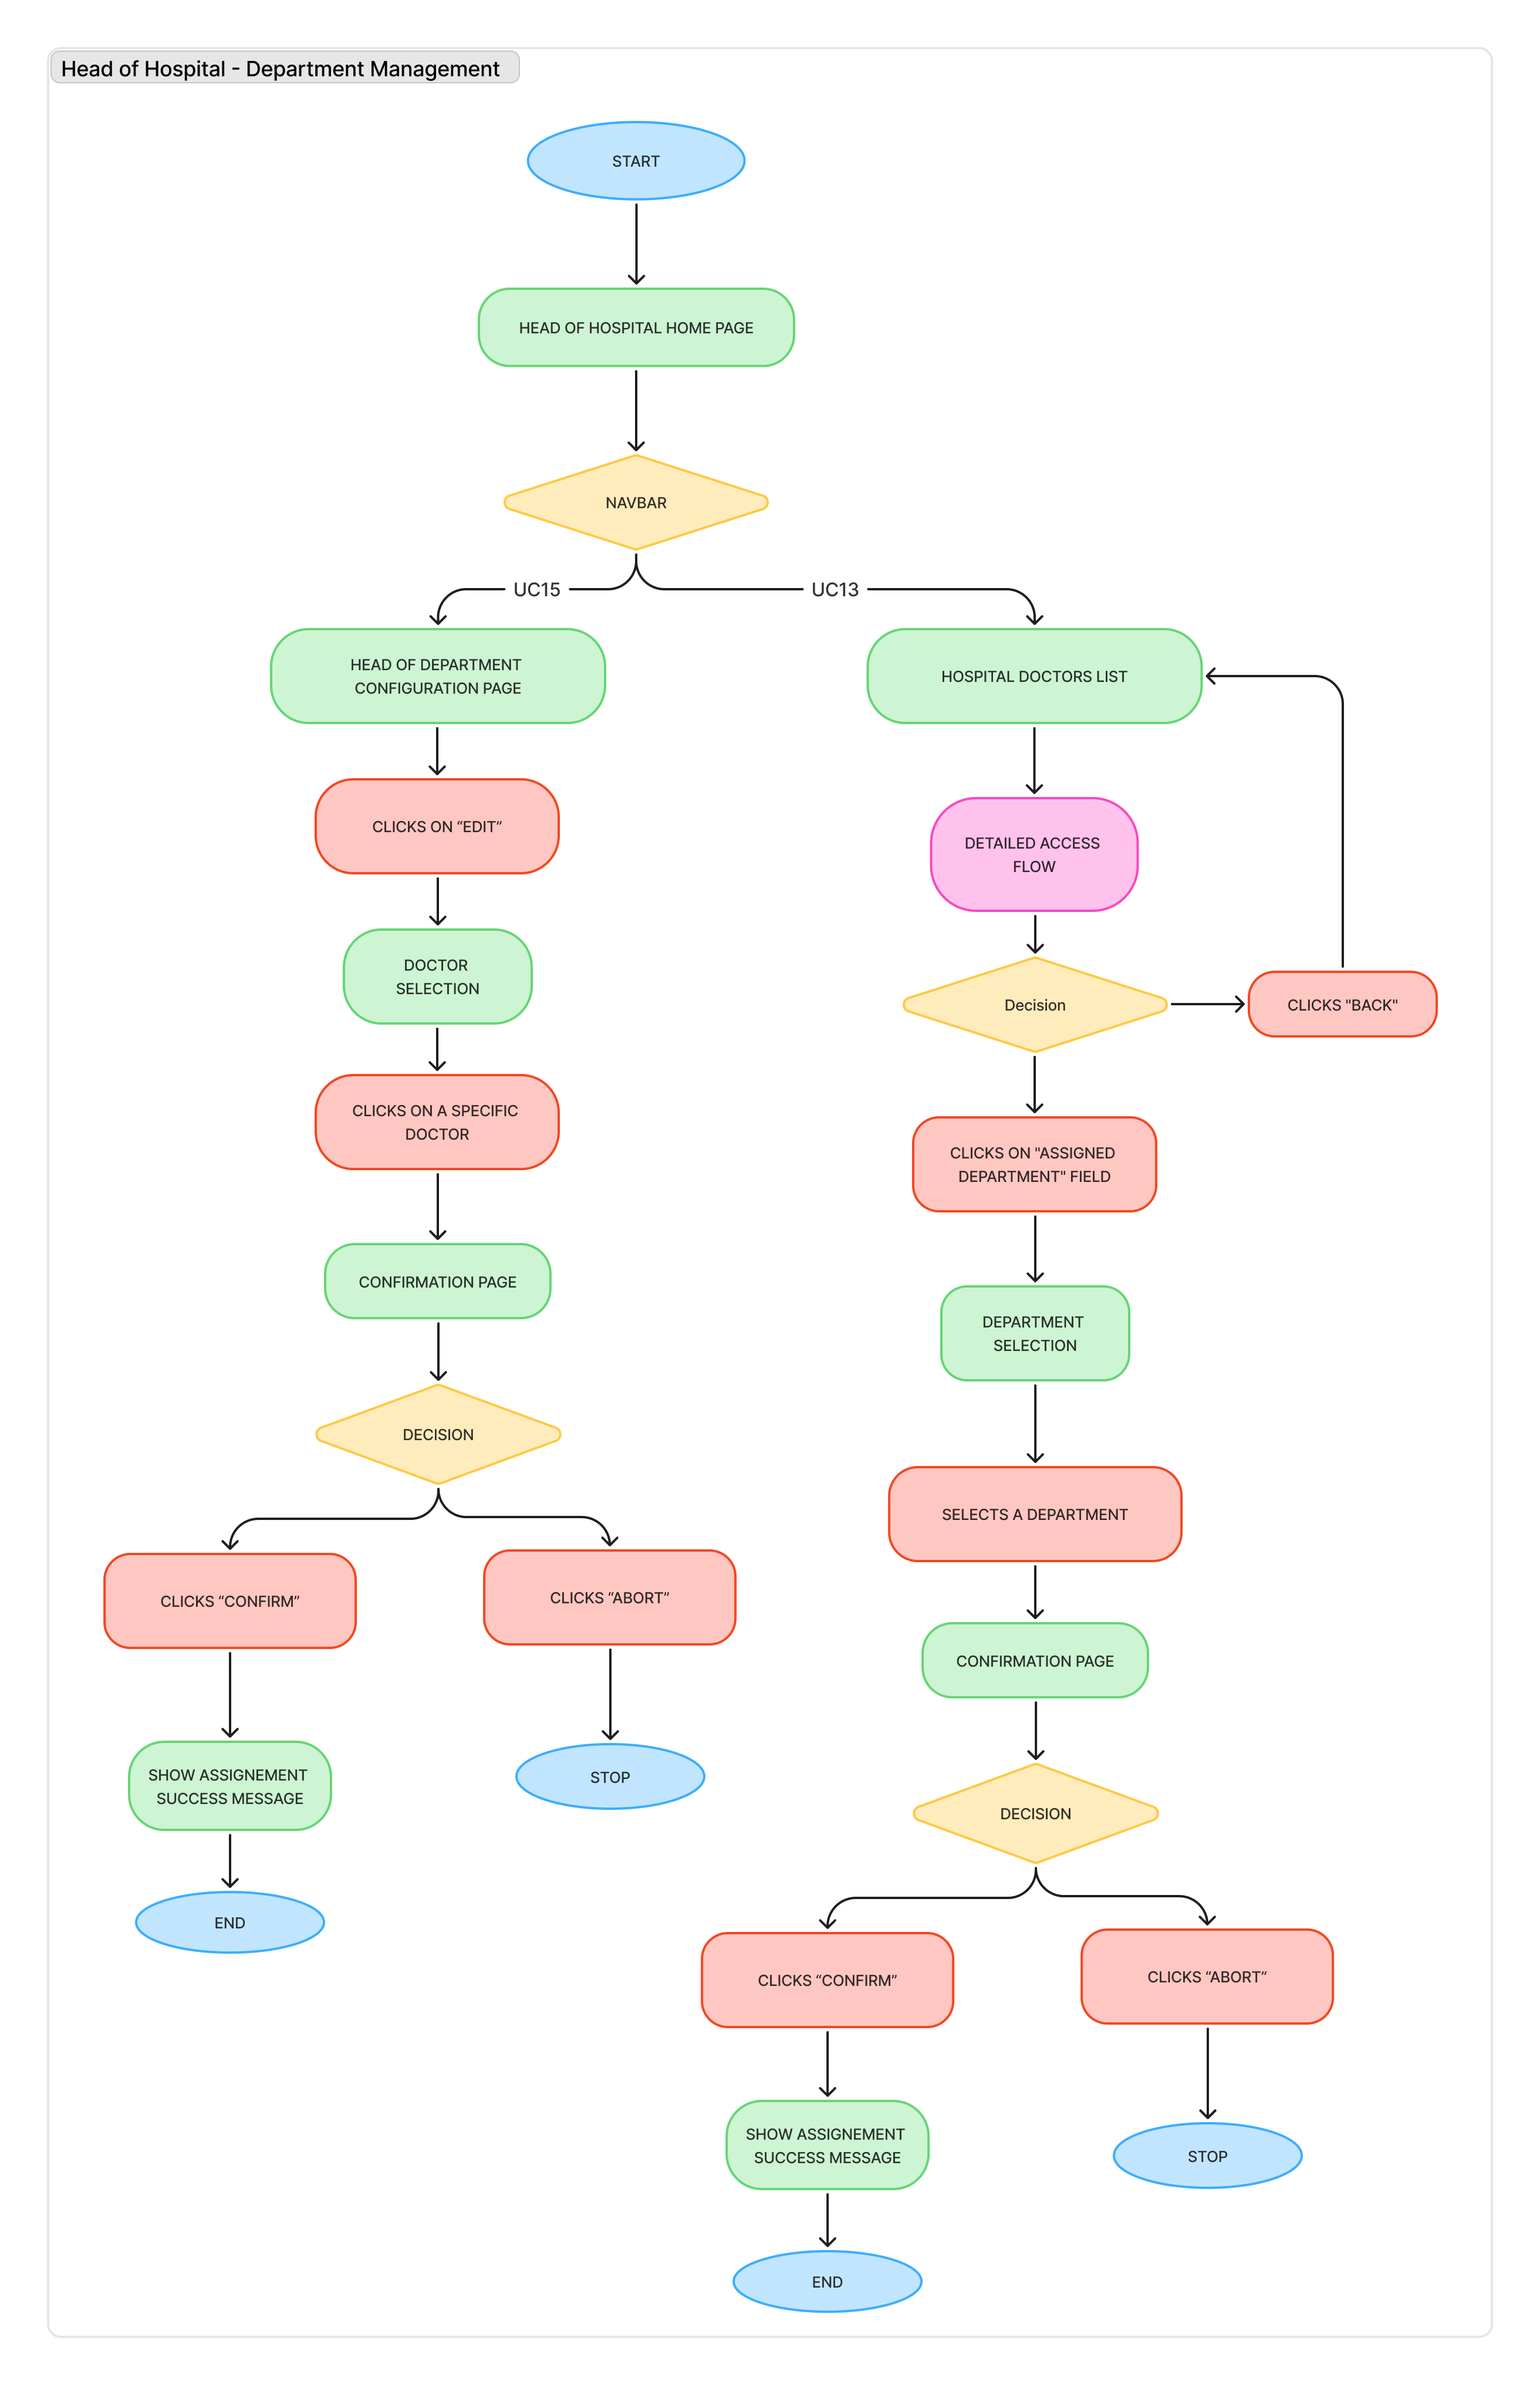
\includegraphics[width=0.7\textwidth]{User_Flows/HospitalHeadAssignements.png}
        \captionof{figure}{User flow regarding Head of Hospital Department Assignments Management}
    \end{center}
    %\begin{itemize}   
    %\end{itemize}
\end{minipage}
\vspace{3em}

\phantomsection
\section{Code Development}
Below are the various APIs developed from the class diagrams and models of D2.
\subsection{Treatment, Hospital, and Department Management}

\begin{figure}[H]
    \centering
    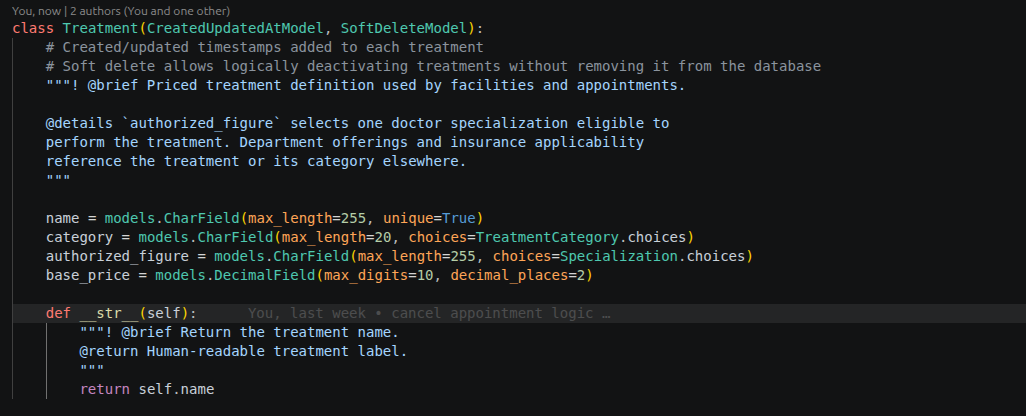
\includegraphics[width=\textwidth]{ScreenshotD3/code_snippets/treatmentModel.png}
    \caption{Treatment model definition declaring the necessary attributes.}
    \label{fig:treatment_model}
\end{figure}

\begin{figure}[H]
    \centering
    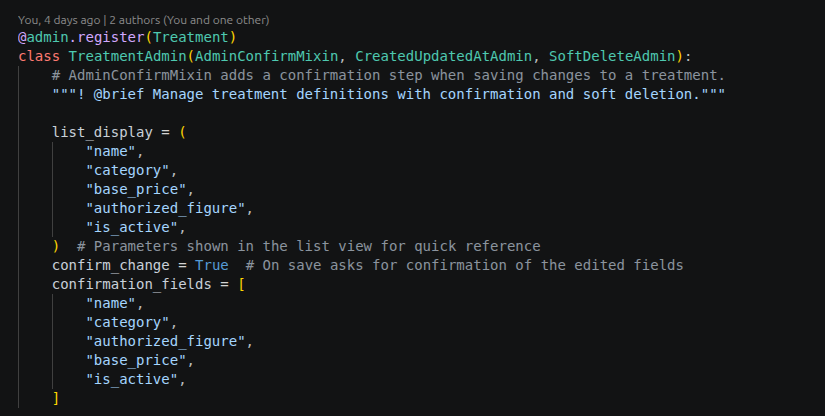
\includegraphics[width=\textwidth]{ScreenshotD3/code_snippets/treatmentAdmin.png}
    \caption{Treatment admin configuration utilizing mixins for soft deletion and edit confirmation.}
    \label{fig:treatment_admin}
\end{figure}

The functionality allowing an administrator to manage treatments, hospitals, and departments follows a consistent pattern across the application:

\begin{itemize}
    \item The model defines the relevant class attributes.
    \item The Django admin automatically generates the interface for entity creation. Non-default behaviors---such as soft deletion and edit confirmation prompts---are implemented using custom admin classes and mixins.
\end{itemize}

The management functionalities for Hospitals and Departments are implemented using the exact same approach; the primary difference lies solely in the specific attributes declared within their respective models.

\vspace{0.5cm}
\noindent\textbf{Linked Use Cases:}
\begin{itemize}
    \item \textbf{UC1} - Create Treatment / Hospital / Department
    \item \textbf{UC5} - Edit Treatment / Hospital / Department
    \item \textbf{UC8} - Deactivate or close Treatment / Hospital / Department
\end{itemize}

\phantomsection
\subsection{Insurance Policy Administration Management}

\begin{figure}[H]
    \centering
    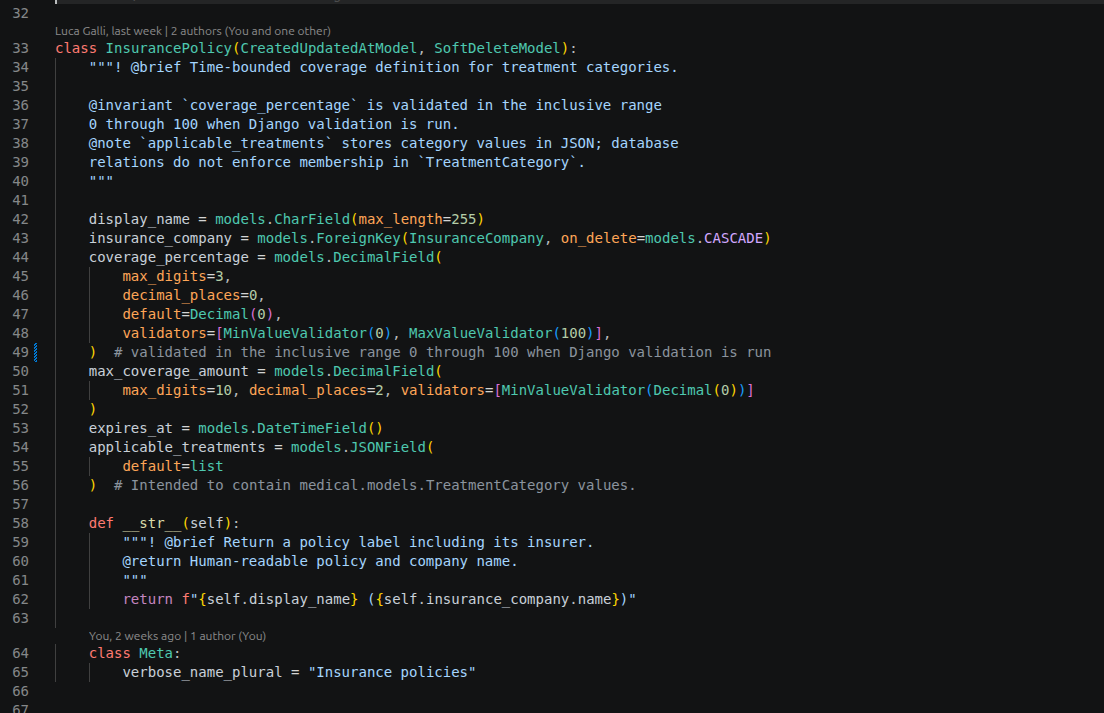
\includegraphics[width=\textwidth]{ScreenshotD3/code_snippets/policyModel.png}
    \caption{Insurance Policy model definition declaring the necessary attributes and validators.}
    \label{fig:policy_model}
\end{figure}

\begin{figure}[H]
    \centering
    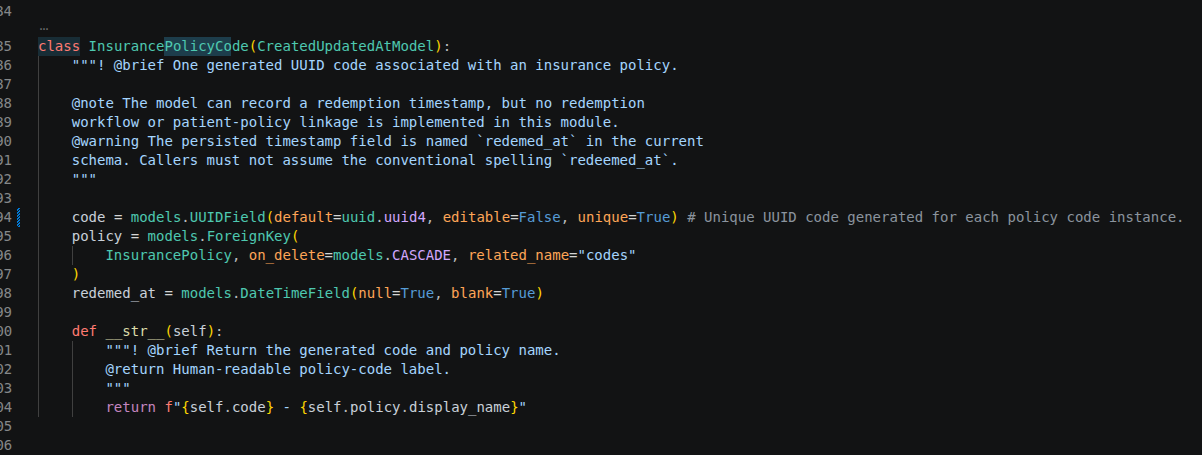
\includegraphics[width=\textwidth]{ScreenshotD3/code_snippets/policyCodeModel.png}
    \caption{Insurance Policy Code model definition.}
    \label{fig:policy_code_model}
\end{figure}

\begin{figure}[H]
    \centering
    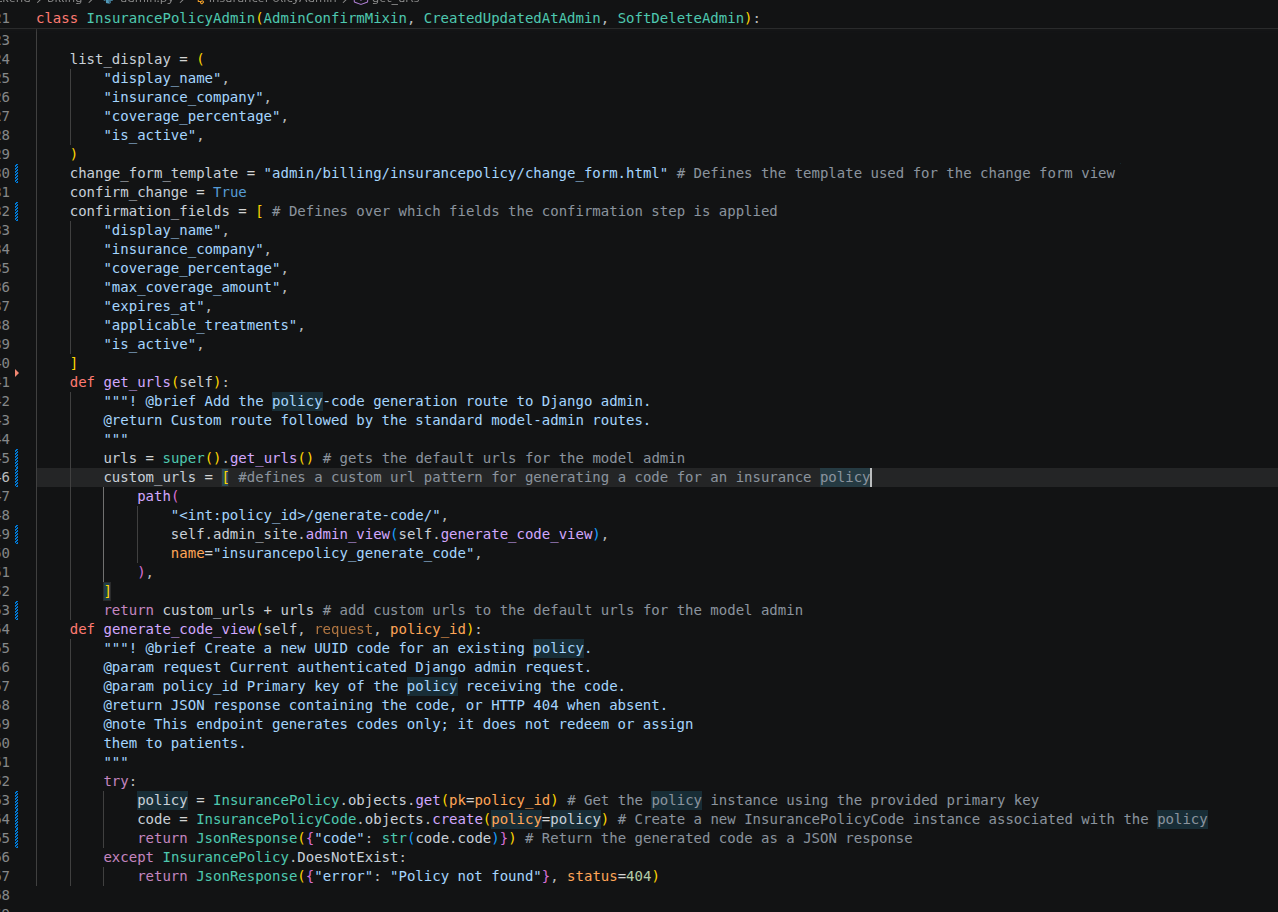
\includegraphics[width=\textwidth]{ScreenshotD3/code_snippets/policyAdmin.png}
    \caption{Insurance Policy admin configuration utilizing mixins and custom endpoints.}
    \label{fig:policy_admin}
\end{figure}

It is worth noting that specific field-level validations have been integrated directly into the models to strictly enforce the business rules outlined in the use cases. For instance, the \texttt{coverage\_percentage} is constrained within an inclusive range of 0 to 100.

Furthermore, the administration interface for insurance policies is notably more complex than standard entities to accommodate the dynamic generation of policy codes. This complexity is managed through several key customizations:

\begin{itemize}
    \item \textbf{Custom UI Integration:} The admin class defines a \texttt{change\_form\_template} to utilize a custom HTML layout. This allows the injection of specific UI elements directly within the standard Django edit form.
    \item \textbf{Custom Routing:} The \texttt{get\_urls()} method is overridden to append a new, protected API endpoint (\texttt{<int:policy\_id>/generate-code/}) to the standard model-admin URL patterns.
    \item \textbf{Dedicated View Logic:} The \texttt{generate\_code\_view()} method acts as the controller for this new route. It securely fetches the requested policy instance, generates a unique, one-off \texttt{InsurancePolicyCode} (UUID), and returns it to the client as a JSON response.
\end{itemize}

\vspace{0.5cm}
\noindent\textbf{Linked Use Cases:}
\begin{itemize}
    \item \textbf{UC2} - Create Insurance Policy
    \item \textbf{UC6} - Update Insurance Policy
    \item \textbf{UC9} - Deactivate Insurance Policy
    \item \textbf{UC22} - Generate Insurance Policy Code
\end{itemize}

\phantomsection
\subsection{Doctor Creates Prescription / Exemption / Examination}

\begin{figure}[H]
    \centering
    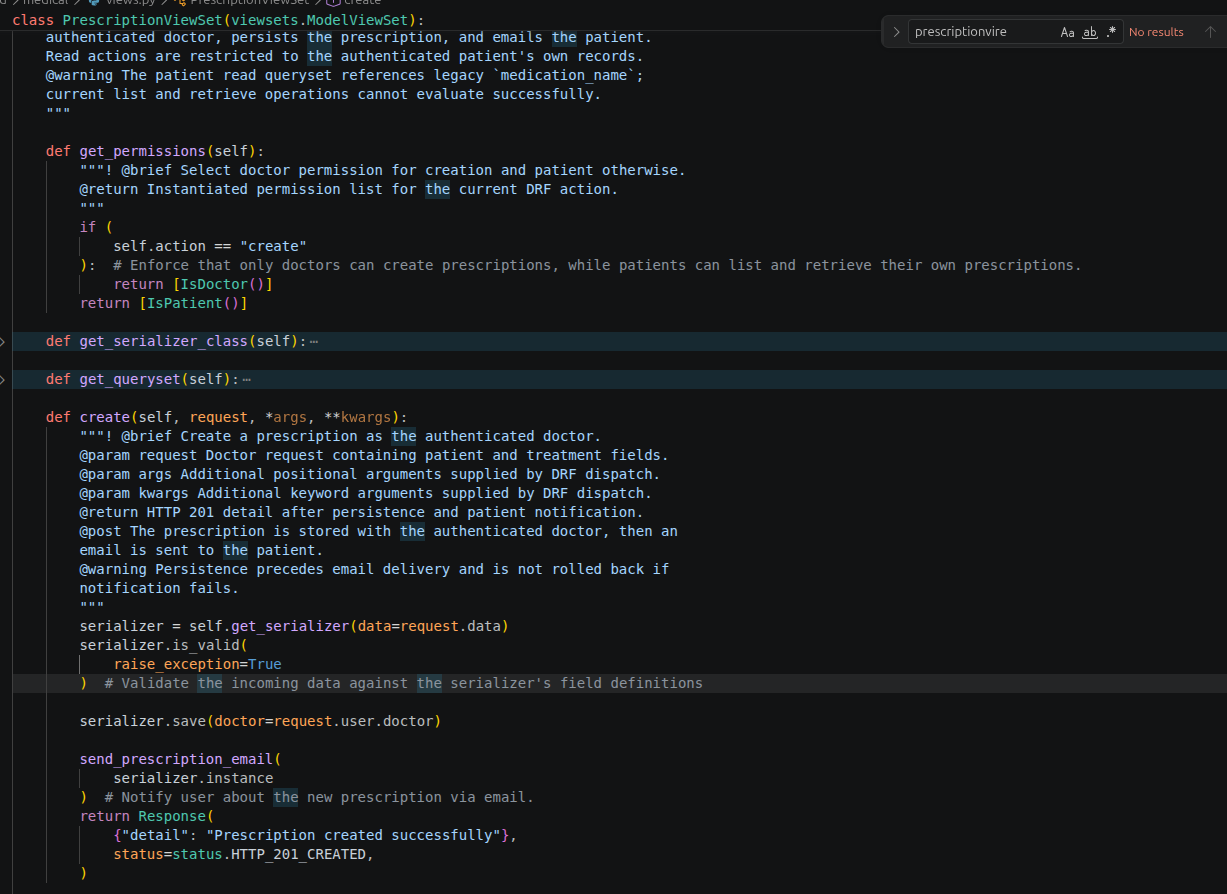
\includegraphics[width=\textwidth]{ScreenshotD3/code_snippets/prescriptionCreateView.png}
    \caption{Prescription creation view implementation.}
    \label{fig:prescription_create_view}
\end{figure}

\begin{figure}[H]
    \centering
    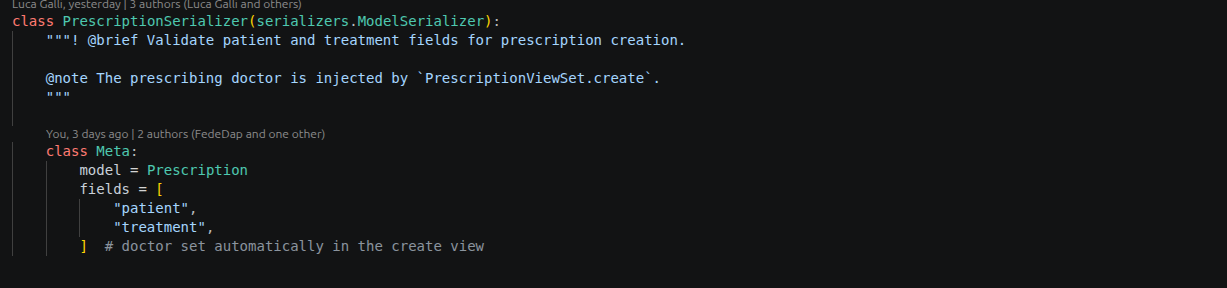
\includegraphics[width=\textwidth]{ScreenshotD3/code_snippets/prescriptionCreateSerializer.png}
    \caption{Prescription creation serializer implementation.}
    \label{fig:prescription_create_serializer}
\end{figure}

\begin{figure}[H]
    \centering
    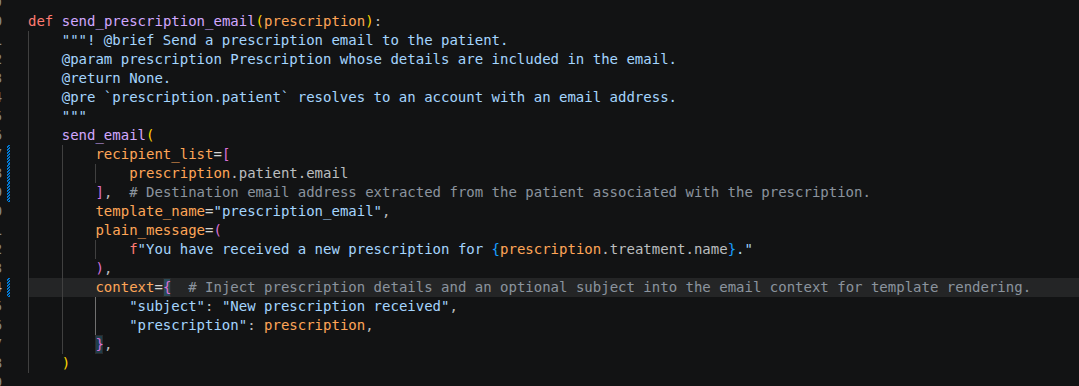
\includegraphics[width=\textwidth]{ScreenshotD3/code_snippets/prescriptionEmail.png}
    \caption{Prescription email notification implementation.}
    \label{fig:prescription_email}
\end{figure}

The creation of a prescription is handled by a dedicated DRF \texttt{ViewSet} that overrides both the permission logic and the \texttt{create()} method to enforce the business rules associated with this use case.

\begin{itemize}
    \item \textbf{Permission Enforcement:} The \texttt{get\_permissions()} method dynamically selects the applicable permission class based on the requested action. Only authenticated doctors are allowed to perform the \texttt{create} action, while patients retain read-only access (list and retrieve) restricted to their own prescriptions.
    \item \textbf{Serializer Validation:} The \texttt{PrescriptionSerializer} exposes only the \texttt{patient} and \texttt{treatment} fields to the client. The prescribing doctor is deliberately excluded from the writable fields, as it is automatically injected server-side from the authenticated user.
    \item \textbf{Creation Logic:} The overridden \texttt{create()} method validates the incoming payload, persists the prescription by associating it with the doctor profile of the authenticated user (\texttt{request.user.doctor}), and finally triggers an email notification to the patient.
    \item \textbf{Email Notification:} The \texttt{send\_prescription\_email()} function retrieves the patient's email address from the prescription instance and dispatches a templated email informing them of the new prescription, including the treatment name in the message body and context.
\end{itemize}

\vspace{0.2cm}

\vspace{0.2cm}
\noindent The management of Exemptions and examinations follows the exact same approach described above; the \texttt{ViewSet}, serializer, and email notification logic mirror the structure shown for Prescriptions, with the only difference being the specific model and fields involved.

\vspace{0.5cm}
\noindent\textbf{Linked Use Cases:}
\begin{itemize}
    \item \textbf{UC3} - Create Prescription / Exemption
    \item \textbf{UC4} - Upload Examination
\end{itemize}


\phantomsection
\subsection{Account Management}

\begin{figure}[H]
    \centering
    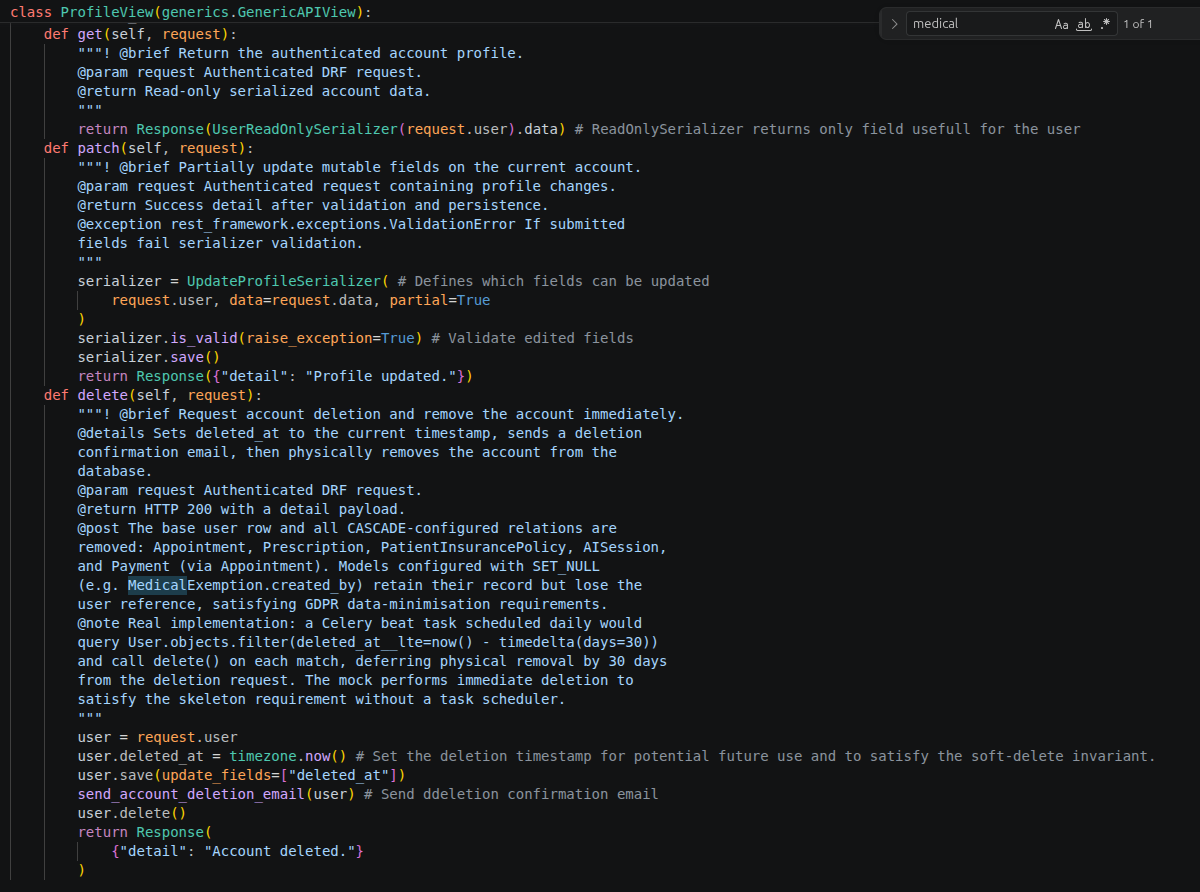
\includegraphics[width=\textwidth]{ScreenshotD3/code_snippets/profileActions.png}
    \caption{Profile actions implementation.}
    \label{fig:profile_actions}
\end{figure}

\begin{figure}[H]
    \centering
    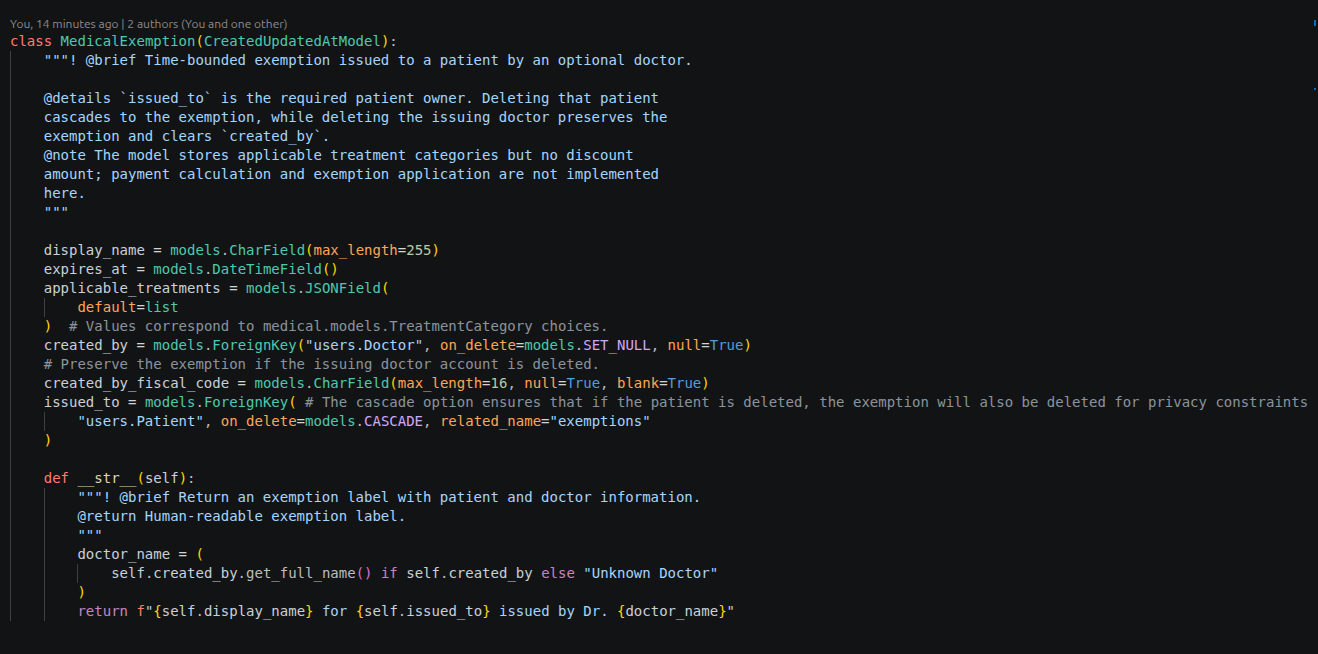
\includegraphics[width=\textwidth]{ScreenshotD3/code_snippets/exemptionModel.png}
    \caption{Medical Exemption model definition showing the \texttt{CASCADE} and \texttt{SET\_NULL} relations used for cascading deletion.}
    \label{fig:medical_exemption_model}
\end{figure}

To satisfy \textbf{NFR0 - Security and Privacy} and to enforce GDPR compliance, account deletion has been designed to support a \textit{soft delete} mechanism.

\begin{itemize}
\item \textbf{Soft Delete Flag:} The data model already includes a \texttt{deleted\_at} timestamp field, intended to mark an account as pending deletion without immediately destroying the underlying data. In the current implementation, however, the \texttt{delete()} handler of \texttt{ProfileView} sets this timestamp and then immediately proceeds with the physical deletion of the account (\texttt{user.delete()}), after sending a confirmation email to the user via \texttt{send\_account\_deletion\_email()}. The flag is therefore already in place to support the grace-period mechanism described below, even though it is not yet leveraged to defer the actual deletion.    \item \textbf{Future Periodic Cleanup:} In the intended production implementation, a periodic Celery beat task would run daily, querying for all users whose \texttt{deleted\_at} timestamp is older than 30 days (\texttt{User.objects.filter(deleted\_at\_\_lte=now() - timedelta(days=30))}) and physically deleting them. 
    \item \textbf{Mock Behavior:} Since no task scheduler is included in this skeleton, the current implementation performs the physical deletion (\texttt{user.delete()}) immediately after setting \texttt{deleted\_at}, in order to demonstrate the cascading behavior described below without requiring Celery infrastructure.
\end{itemize}

\vspace{0.2cm}
\noindent\textbf{Cascading Data Removal.} The physical deletion of the user record triggers a cascade of deletions across all related entities, as configured at the model level via \texttt{on\_delete} relations. As shown in Figure~\ref{fig:medical_exemption_model} for the \texttt{MedicalExemption} model, two distinct strategies are applied depending on the nature of the relationship:

\begin{itemize}
    \item \textbf{CASCADE:} Models that represent data intrinsically owned by the deleted account are configured with \texttt{on\_delete=models.CASCADE}. When the patient account is removed, all of these related records are deleted along with it, ensuring no personal data is left behind.
    \item \textbf{SET\_NULL:} Conversely, models that may need to be preserved for medical or administrative continuity are configured with \texttt{on\_delete=models.SET\_NULL}. If the issuing doctor's account is deleted, the exemption record itself is retained, but the foreign key reference is cleared, satisfying the GDPR data-minimisation principle while preserving the exemption for the patient.
\end{itemize}

\vspace{0.5cm}
\noindent\textbf{Linked Use Cases:}
\begin{itemize}
    \item \textbf{UC7} - Update User profile
    \item \textbf{UC41} - Account Deletion
\end{itemize}



\phantomsection
\subsection{Registration and Validation}

\begin{figure}[H]
    \centering
    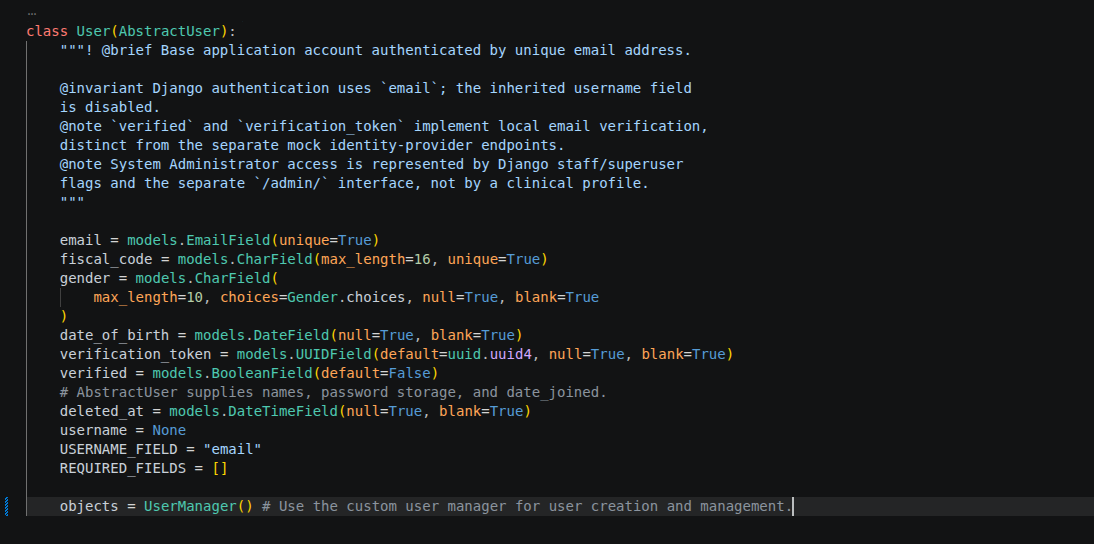
\includegraphics[width=\textwidth]{ScreenshotD3/code_snippets/userClass.png}
    \caption{User class definition showing the attributes and methods for user management.}
    \label{fig:user_class}
\end{figure}
\begin{figure}[H]
    \centering
    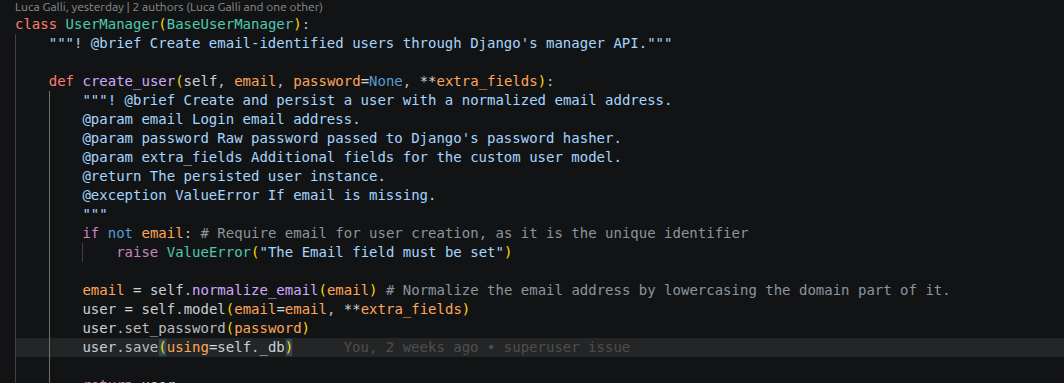
\includegraphics[width=\textwidth]{ScreenshotD3/code_snippets/userManager.png}
    \caption{User manager implementation showing the custom user creation logic.}
    \label{fig:user_manager}
\end{figure}
\begin{figure}[H]
    \centering
    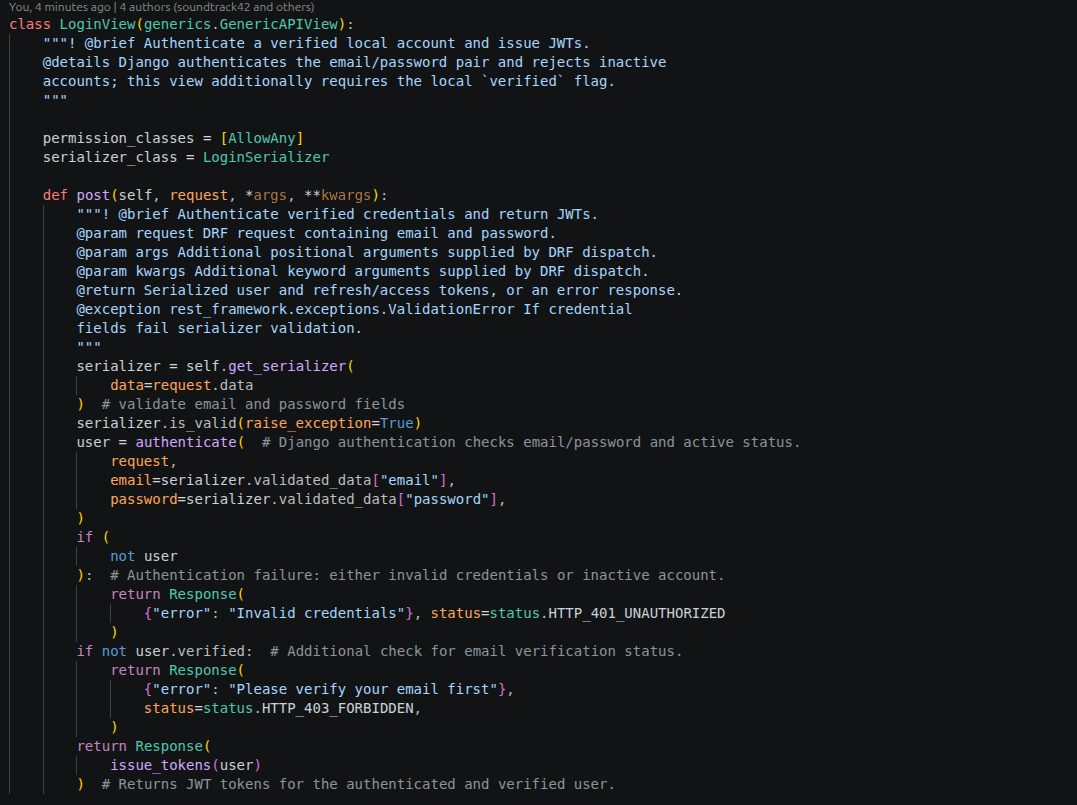
\includegraphics[width=\textwidth]{ScreenshotD3/code_snippets/loginView.png}
    \caption{Login view implementation showing the user authentication logic.}
    \label{fig:login_view}
\end{figure}
\begin{figure}[H]
    \centering
    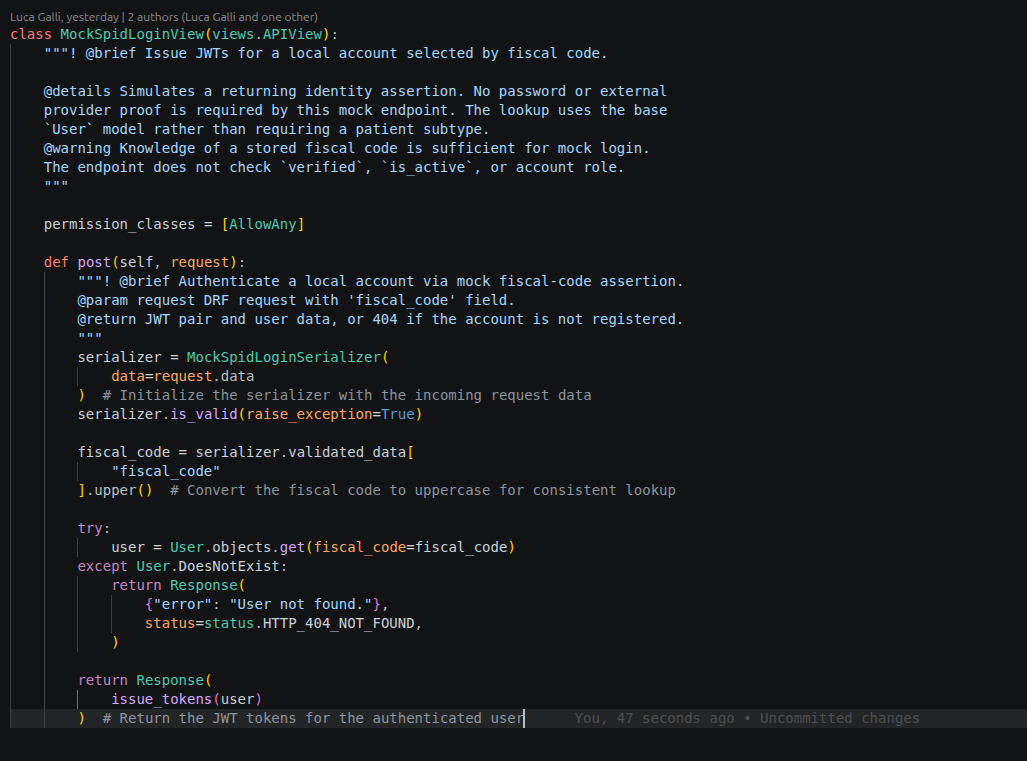
\includegraphics[width=\textwidth]{ScreenshotD3/code_snippets/mockLogin.png}
    \caption{Mock SPID login implementation.}
    \label{fig:mock_login}
\end{figure}
\begin{figure}[H]
    \centering
    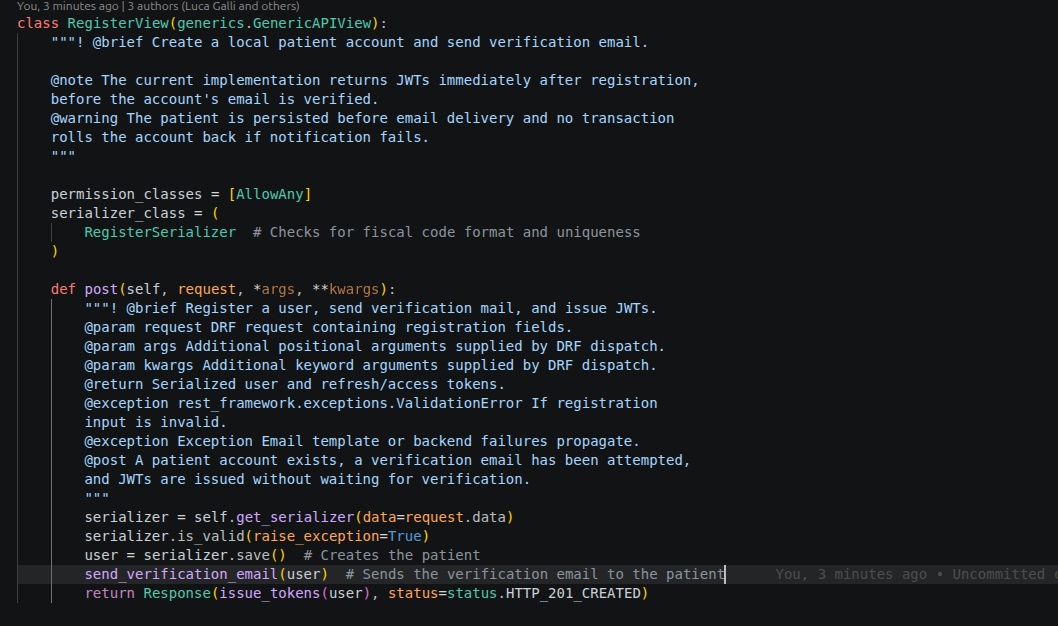
\includegraphics[width=\textwidth]{ScreenshotD3/code_snippets/registerView.png}
    \caption{Registration view implementation showing the user registration logic.}
    \label{fig:register_view}
\end{figure}
\begin{figure}[H]
    \centering
    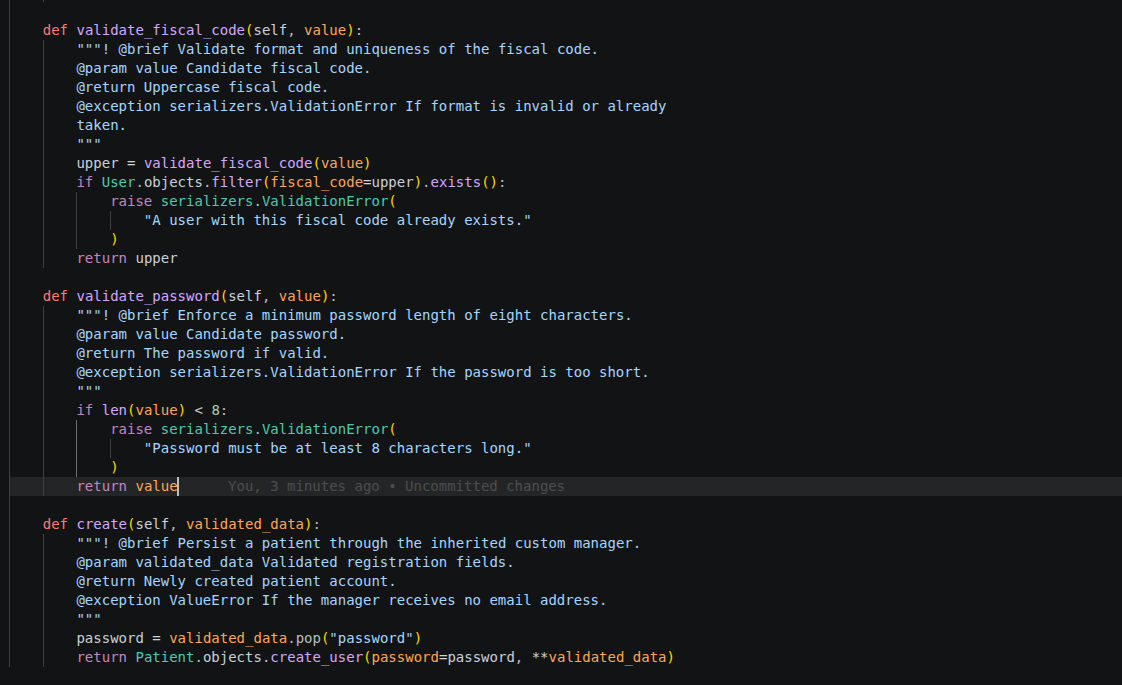
\includegraphics[width=\textwidth]{ScreenshotD3/code_snippets/registerSerializer.png}
    \caption{Registration serializer implementation showing the validation logic.}
    \label{fig:register_serializer}
\end{figure}
\begin{figure}[H]
    \centering
    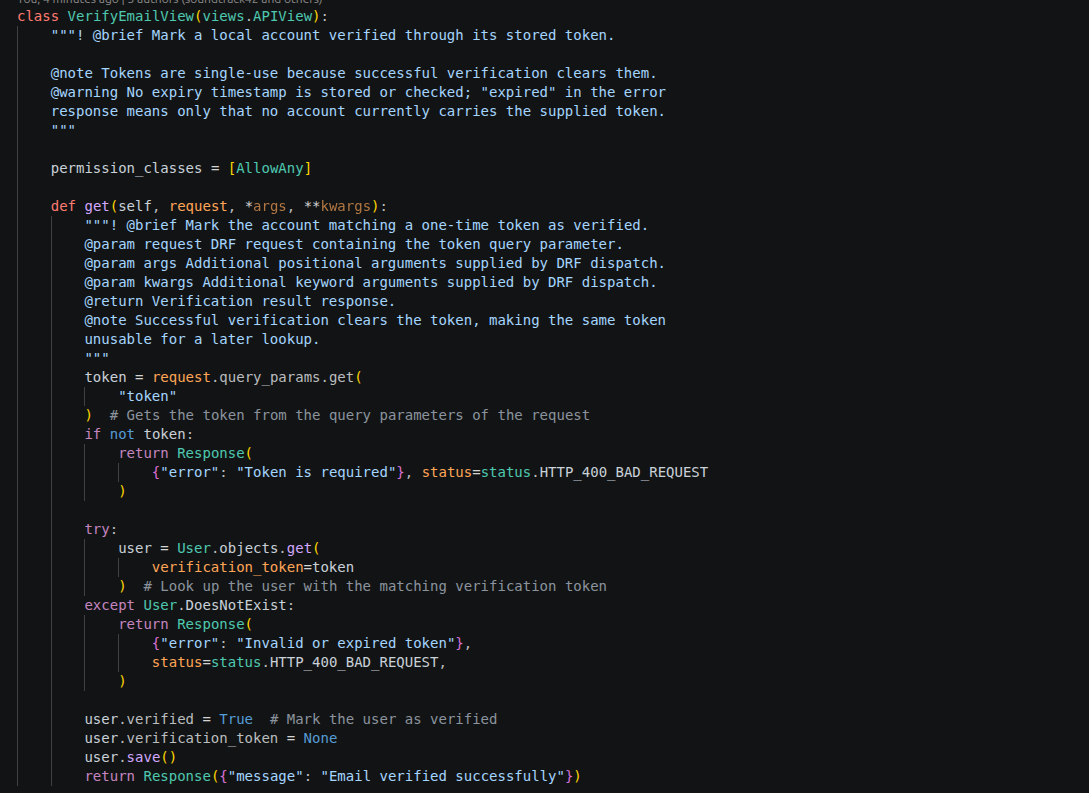
\includegraphics[width=\textwidth]{ScreenshotD3/code_snippets/verifyEmail.png}
    \caption{Email verification implementation showing the verification logic.}
    \label{fig:verify_email}
\end{figure}
\begin{figure}[H]
    \centering
    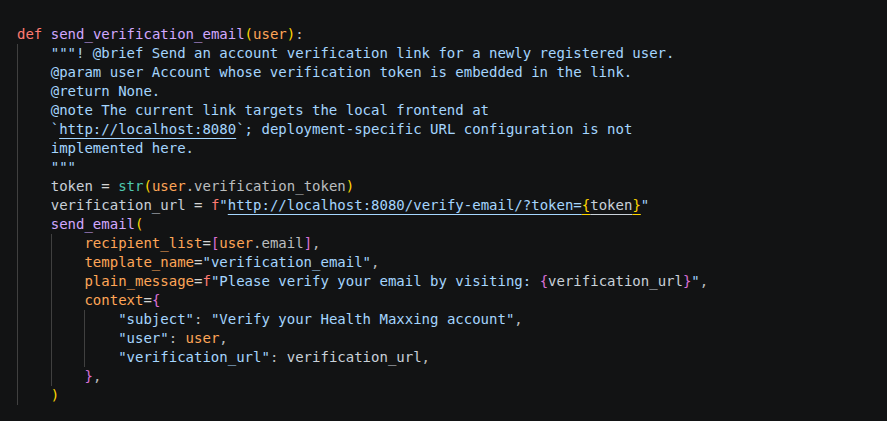
\includegraphics[width=\textwidth]{ScreenshotD3/code_snippets/sendVerificationEmail.png}
    \caption{Email verification implementation showing the verification logic.}
    \label{fig:send_verification_email}
\end{figure}

The \texttt{User} model extends Django's \texttt{AbstractUser} and is configured to authenticate via \texttt{email} instead of a username, which is explicitly disabled by setting \texttt{USERNAME\_FIELD = "email"} and \texttt{username = None}. In addition to the fields inherited from \texttt{AbstractUser} (such as name and password storage), the model defines application-specific attributes: a unique \texttt{fiscal\_code}, an optional \texttt{gender} and \texttt{date\_of\_birth}, and the pair \texttt{verified} / \texttt{verification\_token}, which together implement local email verification independently from the mock identity-provider endpoints. User creation is delegated to a custom \texttt{UserManager}, which normalizes the email address, enforces its presence, and hashes the password before persisting the account.

\vspace{0.2cm}
\noindent\textbf{Registration.} The \texttt{RegisterView} exposes an open (\texttt{AllowAny}) endpoint that validates the incoming payload through \texttt{RegisterSerializer} --- which checks the format and uniqueness of the fiscal code --- and persists the new patient account. Immediately after creation, \texttt{send\_verification\_email()} is called to deliver a verification link containing the account's \texttt{verification\_token}.

\vspace{0.2cm}
\noindent\textbf{Email Verification.} The \texttt{send\_verification\_email()} function builds a one-time verification URL embedding the user's \texttt{verification\_token} and dispatches it via the templated email system. The corresponding \texttt{VerifyEmailView} exposes a public endpoint that looks up the account matching the token supplied as a query parameter; if found, the account is marked as \texttt{verified} and its token is cleared, making it single-use. If no account matches the supplied token, a generic ``invalid or expired token'' error is returned.

\vspace{0.2cm}
\noindent\textbf{Login.} The \texttt{LoginView} validates the submitted email and password through \texttt{LoginSerializer} and then relies on Django's \texttt{authenticate()} to verify the credentials and the account's active status. On top of this, the view performs an additional check on the local \texttt{verified} flag: if the credentials are valid but the account has not yet completed email verification, an HTTP 403 response is returned instructing the user to verify their email first. Only after passing both checks are JWT tokens issued to the client via \texttt{issue\_tokens()}.

\vspace{0.5cm}
\noindent\textbf{Linked Use Cases:}
\begin{itemize}
    \item \textbf{UC23} - User Registration and Validation
    \item \textbf{UC24} - User Login
\end{itemize}

\phantomsection
\subsection{Medical Record access}

\begin{figure}[H]
    \centering
    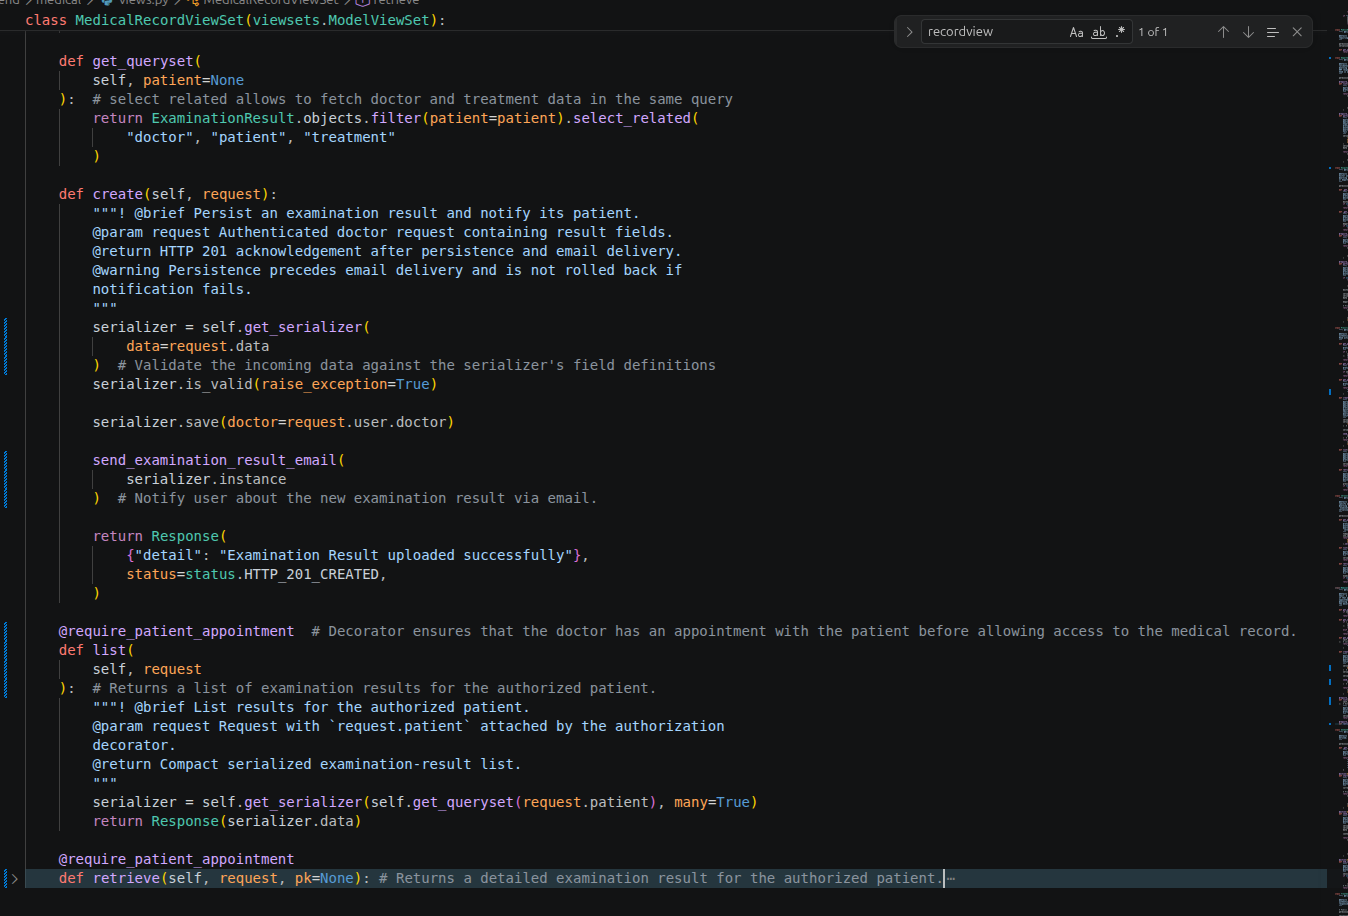
\includegraphics[width=\textwidth]{ScreenshotD3/code_snippets/recordView.png}
    \caption{Medical record access implementation showing the record view.}
    \label{fig:record_view}
\end{figure}
\begin{figure}[H]
    \centering
    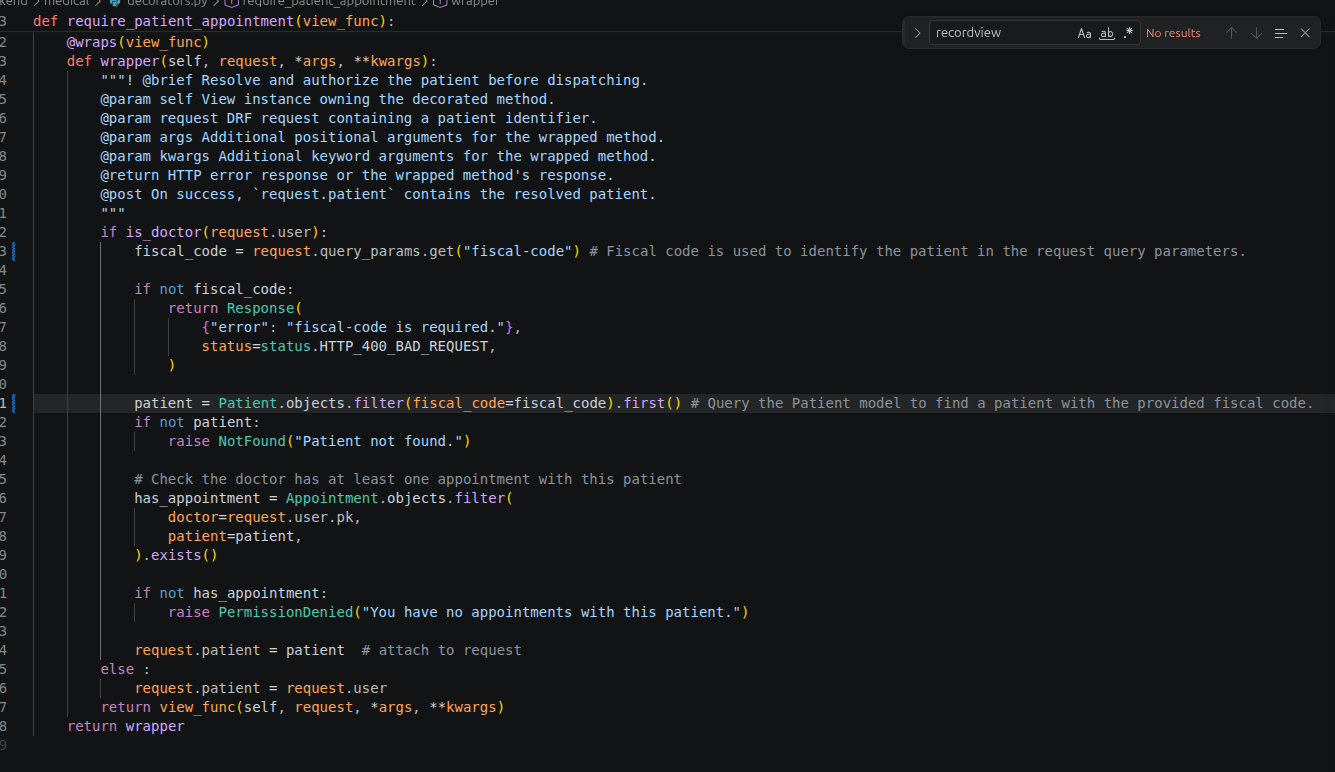
\includegraphics[width=\textwidth]{ScreenshotD3/code_snippets/requireAppointmentWrap.png}
    \caption{Appointment requirement implementation.}
    \label{fig:require_appointment_wrap}
\end{figure}

Access to medical records (examination results) is handled by \texttt{MedicalRecordViewSet}, which differentiates behavior based on both the requested action and the role of the authenticated user.

\begin{itemize}
    \item \textbf{Permission Enforcement:} The \texttt{get\_permissions()} method restricts the \texttt{create} action to doctors only (\texttt{IsDoctor}), while all other actions simply require an authenticated user (\texttt{IsAuthenticated}), since both patients and doctors are allowed to read records, subject to the additional authorization described below.
    \item \textbf{Serializer Selection:} The \texttt{get\_serializer\_class()} method returns a different serializer depending on the action: a fully validated \texttt{ExaminationResultSerializer} is used for creation, a lightweight \texttt{ExaminationResultListSerializer} is used for listing, and a more detailed \texttt{ExaminationResultDetailSerializer} is used for retrieving a single record.
    \item \textbf{Creation Logic:} The \texttt{create()} method validates the incoming payload, persists the examination result associating it with the authenticated doctor (\texttt{request.user.doctor}), and notifies the patient by calling \texttt{send\_examination\_result\_email()}. As with other notification flows in the system, persistence precedes email delivery and is not rolled back if the notification fails.
    \item \textbf{Queryset Construction:} The \texttt{get\_queryset()} method filters \texttt{ExaminationResult} objects by the resolved patient and uses \texttt{select\_related()} on \texttt{doctor}, \texttt{patient}, and \texttt{treatment} to avoid additional queries when serializing related data.
\end{itemize}

\vspace{0.2cm}
\noindent\textbf{Authorization via \texttt{require\_patient\_appointment}.} The \texttt{list()} and \texttt{retrieve()} actions are wrapped by the \texttt{require\_patient\_appointment} decorator, which is responsible for resolving \emph{whose} medical records the request is allowed to access and attaching the result to \texttt{request.patient}:

\begin{itemize}
    \item \textbf{Patient Requests:} If the authenticated user is not a doctor, they are assumed to be a patient, and \texttt{request.patient} is simply set to \texttt{request.user}, granting access to their own records.
    \item \textbf{Doctor Requests:} If the authenticated user is a doctor, the request must include a \texttt{fiscal-code} query parameter identifying the target patient. The decorator looks up the corresponding \texttt{Patient} record (raising \texttt{NotFound} if it does not exist) and then verifies that the doctor has at least one \texttt{Appointment} with that patient, raising \texttt{PermissionDenied} otherwise.
\end{itemize}

\vspace{0.2cm}

\vspace{0.5cm}
\noindent\textbf{Linked Use Cases:}
\begin{itemize}
    \item \textbf{UC40} - Medical Record Access (patient)
    \item \textbf{UC42} - Medical record access (doctor)
\end{itemize}
\phantomsection 
\section{Team Assessment}

\phantomsection 
\subsection{Work organization}

In the early stages of the project, the work was divided mainly according to:

\begin{itemize}
    \item equal division of the workload;
    \item assignment based on the basic skills that each person had;
    \item affinity for a specific task.
\end{itemize}

Maintaining the last two criteria mentioned above, it was subsequently decided to modify the first point by opting for a division of work based on the time available. To coordinate, we held weekly meetings either on Discord or in person. As the project progressed into the implementation and final phases, the frequency of meetings increased in order to better synchronize the work and address issues more promptly.

\phantomsection 
\subsection{Roles and activities}

\begin{table}[H]
\centering
\begin{tabular}{|p{2cm}|p{10cm}|}
\hline
\rowcolor{gray!50}
\textbf{Team Member} & \textbf{Main activities} \\
\hline
Stefano & Assigning and reviewing tasks, writing functional and non-functional requirements, writing use cases, front-end and back-end development \\
\hline
Federico & Proofreading of all deliverables: covering syntactic, logical, and grammatical inconsistencies, writing use cases, writing functional and non-functional requirements, creating user flows, creating the project boundary diagram, back-end development \\
\hline
Giorge & Creating activity diagrams, creating sequence diagrams, writing functional and non-functional requirements, creating ER diagram, front-end and back-end development (minor contribution) \\
\hline
Luca & Creation of the class diagram, front-end and back-end development, defining requirements, defining architectural and language design choices, writing project objectives \\
\hline
\end{tabular}
\end{table}

\phantomsection 
\subsection{Workload and distribution}

Below is the workload expressed in percentage per deliverable for each member of the group.

\begin{table}[H]
\centering
\begin{tabular}{|p{3cm}|p{2cm}|p{2cm}|p{2cm}|p{2cm}|}
\hline
\rowcolor{gray!50}
 & \textbf{Stefano} & \textbf{Federico} & \textbf{Giorge} & \textbf{Luca} \\
\hline
D1 & 25 & 25 & 25 & 25 \\
\hline
D2 & 25 & 30 & 30 & 15 \\
\hline
D3 & 25 & 20 & 20 & 35 \\
\hline
\rowcolor{red!20}
\textbf{Proposed grade} & 30 & 30 & 30 & 30 \\
\hline
\end{tabular}
\end{table}

From the distribution of the participation described in the table, we can see that, except on the D1, the work was never perfectly balanced looking at the single deliverables. But indeed looking at it overall was performed equally by all members.


\end{document}